\documentclass[11pt]{report}
\usepackage[margin=1.1in]{geometry}
\usepackage[utf8]{inputenc}
\usepackage[italian]{babel}
\usepackage{amssymb} 
\usepackage{amsmath}
\usepackage{amsthm}
\usepackage{thmtools}
\usepackage{multicol}
%\usepackage{marginnote}
\usepackage{pdfpages}
\usepackage{graphicx}
\usepackage{makecell}

\usepackage{hyperref}
\usepackage{fancyvrb}
\usepackage{subcaption}
%\usepackage[linktocpage=true]{hyperref}

\theoremstyle{definition}
\newtheorem*{definizione}{Definizione}
\usepackage{thmtools}

\DeclareRobustCommand{\ojoin}{\rule[0.10ex]{.3em}{.4pt}\llap{\rule[1.40ex]{.3em}{.4pt}}}
\newcommand{\leftouterjoin}{\mathrel{\ojoin\mkern-6.5mu\Join}}
\newcommand{\rightouterjoin}{\mathrel{\Join\mkern-6.5mu\ojoin}}
\newcommand{\fullouterjoin}{\mathrel{\ojoin\mkern-6.5mu\Join\mkern-6.5mu\ojoin}}

\setcounter{tocdepth}{3}
\setcounter{secnumdepth}{3}

\usepackage{wrapfig}

\usepackage{titlesec, blindtext, color}
\definecolor{gray75}{gray}{0.75}
\newcommand{\hsp}{\hspace{20pt}}
\titleformat{\chapter}[hang]{\Huge\bfseries}{\thechapter\hsp\textcolor{gray75}{|}\hsp}{0pt}{\Huge\bfseries}

\usepackage[
type={CC},
modifier={by-nc-sa},
version={4.0},
]{doclicense}

\begin{document}
	\title{\textbf{Appunti delle lezioni della Vaglini - Basi di dati}}
	\author{Gabriele Frassi}
	\date{A.A 2019-2020 - Secondo semestre}
	\maketitle

	\begin{abstract}
	La dispensa vuole porsi come strumento per conoscere in maniera approfondita il nucleo multiprogrammato didattico presentato durante il corso di Calcolatori Elettronici. Essa descrive i punti nevralgici del nucleo, cercando di approfondire in alcuni punti. Le fonti utilizzate sono:
	\begin{itemize}
		\item le lezioni dell'ultimo mese di Calcolatori elettronici;
		\item le dispense del professore su \url{https://calcolatori.iet.unipi.it/};
		\item il codice del nucleo.
	\end{itemize}
	Ne approfitto per ringraziare due persone: Alessandro Corsi (per la pazienza che ha avuto nei miei confronti in questi mesi estivi) e Giacomo Sansone (per i suoi appunti, che mi hanno permesso di sistemare alcune parti della dispensa)
	
	\doclicenseThis
\end{abstract}

	
	\tableofcontents

	
\part{Unimap}
\small
\begin{itemize}
	\item \textbf{Mer 04/03/2020 08:30-11:30 (3:0 h)} lezione: Introduzione. Modello relazionale. (GIGLIOLA VAGLINI)
	\item \textbf{Gio 05/03/2020 10:30-12:30 (2:0 h)} non tenuta: Sospensione della didattica (GIGLIOLA VAGLINI)
	\item \textbf{Ven 06/03/2020 14:30-16:30 (2:0 h)} non tenuta: Sospensione della didattica (FRANCESCO PISTOLESI)
	\item \textbf{Mer 11/03/2020 08:30-11:30 (3:0 h)} lezione: Algebra relazionale. (GIGLIOLA VAGLINI)
	\item \textbf{Gio 12/03/2020 10:30-12:30 (2:0 h)} lezione: Introduzione e modalità d'esame. Il DBMS MySQL. Sintassi di una query: il SELECT statement. Processing. Condizioni e connettivi logici. Duplicati e keyword DISTINCT. Il valore NULL. Condizioni sui valori NULL. Gestione e formattazione di date. Funzioni DATEDIFF, PERIOD$\_$DIFF e DATE$\_$FORMAT. Lassi di tempo: la keyword INTERVAL. Shift temporale con DATE$\_$ADD/DATE$\_$SUB, e somma diretta. Condizioni temporali legate all'istante di esecuzione: l'impiego di CURRENT$\_$DATE. (FRANCESCO PISTOLESI)
	\item \textbf{Ven 13/03/2020 14:30-16:30 (2:0 h)} lezione: Funzioni di aggregazione: count, count(distinct), sum, avg, min e max. Ridenominazione. Il problema del record connesso a un valore aggregato. Multi-table querying. Inner join. Processing di una query con inner join. Query con join e condizioni sui record. Alias. Natural join. Cross join. Outer join. (FRANCESCO PISTOLESI)
	\item \textbf{Mer 18/03/2020 08:30-11:30 (3:0 h)} lezione: Calcolo relazionale (GIGLIOLA VAGLINI)
	\item \textbf{Gio 19/03/2020 10:30-12:30 (2:0 h)} esercitazione: Risoluzione ragionata degli esercizi per casa. Formulazione delle condizioni, connettivi logici, condizioni temporali e gestione delle date. Commento al codice. (FRANCESCO PISTOLESI)
	\item \textbf{Ven 20/03/2020 11:30-13:30 (2:0 h)} esercitazione: Progetto di interrogazioni con espressioni algebriche o nel calcolo relazionale (GIGLIOLA VAGLINI)
	\item \textbf{Ven 20/03/2020 14:30-16:30 (2:0 h)} lezione: Self join. Uso degli alias. Join multipli. Derived table. Subquery noncorrelated e correlated. Direttiva IN. Subquery scalari. Processazione in MySQL. Risoluzione mista subquery-join. Common Table Expressions (CTE). (FRANCESCO PISTOLESI)
	\item \textbf{Mer 25/03/2020 08:30-11:30 (3:0 h)} lezione: Progetto: modello concettuale (GIGLIOLA VAGLINI)
	\item \textbf{Gio 26/03/2020 10:30-12:30 (2:0 h)} esercitazione: Risoluzione ragionata degli esercizi per casa su join, subquery e funzioni di aggregazione. Esempio di traduzione passo-passo dalla versione con subquery alla versione join-equivalente. (FRANCESCO PISTOLESI)
	\item \textbf{Ven 27/03/2020 14:30-16:30 (2:0 h)} lezione: Raggruppamento. A cosa serve, come funziona e quando usarlo. La clausola GROUP BY. Condizioni sui gruppi: la HAVING clause. Processing in MySQL. Subquery EXISTS. Query con significato insiemistico. Unione di result set. Implementazione della divisione con doppia subquery NOT EXISTS, e con raggruppamento e subquery di conteggio nella having clause. (FRANCESCO PISTOLESI)
	\item \textbf{Mer 01/04/2020 08:30-11:30 (3:0 h)} lezione: La parte DD di SQL. Ristrutturazione di uno schema ER prima della traduzione. (GIGLIOLA VAGLINI)
	\item \textbf{Gio 02/04/2020 10:30-12:30 (2:0 h)} esercitazione: Risoluzione ragionata degli esercizi su query con raggruppamento con join e subquery. Uso delle CTE. (FRANCESCO PISTOLESI)
	\item \textbf{Ven 03/04/2020 11:30-13:30 (2:0 h)} lezione: Traduzione nel modello logico (GIGLIOLA VAGLINI)
	\item \textbf{Ven 03/04/2020 14:30-16:30 (2:0 h)} lezione: Query complesse. Ruolo nell'analisi predittiva, nei modelli decisionali, nel CRM. Strategie risolutive. Modificatori ANY/ALL. Gestire gli ex aequo. Differenza insiemistica. Introduzione alle stored procedure. Sintassi di CREATE PROCEDURE. Gestione degli statement. La keyword DELIMITER. Visualizzazione di result set su standard output. Chiamata a stored procedure. (FRANCESCO PISTOLESI)
	\item \textbf{Mer 08/04/2020 08:30-11:30 (3:0 h)} esercitazione: Esercizi di progetto, di traduzione e di ridondanza. (GIGLIOLA VAGLINI)
	\item \textbf{Gio 16/04/2020 10:30-12:30 (2:0 h)} esercitazione: Esercitazione sulle query complesse. (FRANCESCO PISTOLESI)
	\item \textbf{Ven 17/04/2020 14:30-16:30 (2:0 h)} lezione: Variabili locali e variabili user-defined in una stored procedure. Assegnamento con set e con select into. Parametri di una stored procedure: in, out, inout. Istruzioni condizionali: if-elseif-else, case. Istruzioni iterative: while, repeat e loop. Istruzioni di salto: leave e iterate. Cursori. Sintassi del comando declare cursor. Handler. Tipologie exit e continue. Ciclo di fetch. Exception handling e comando signal. Errori sqlstate. Not found condition. Stored function. Sintassi del comando create function. Esempio di stored function. Esempio di stored procedure che usa una stored function per realizzare un ranking tramite temporary table. (FRANCESCO PISTOLESI)
	\item \textbf{Mer 22/04/2020 08:30-11:30 (3:0 h)} lezione: Dipendenze funzionali e forme normali delle relazioni. (GIGLIOLA VAGLINI)
	\item \textbf{Gio 23/04/2020 10:30-12:30 (2:0 h)} esercitazione: Esercizi su stored procedure e stored function. Svolgimento di due testi d'esame. (FRANCESCO PISTOLESI)
	\item \textbf{Ven 24/04/2020 14:30-16:30 (2:0 h)} lezione: Introduzione ai database attivi. Trigger. Sintassi dell'istruzione create trigger. Trigger after e before. Meccanismo di scatto. Keyword 'new'. Gestione in sync di un attributo ridondante mediante trigger after e before. Business rule e gestione mediante trigger before. Event. Generalità sull'aggiornamento deferred. Pregi e difetti. Sintassi del comando create event. Scheduling di un event. Recurring event. Significato della direttiva on schedule at/every. Introduzione alle materialized view. Utilità nel reporting e nel data analytics. Performance. Politiche di refresh: immediate, deferred e on demand. (FRANCESCO PISTOLESI)
	\item \textbf{Mer 29/04/2020 08:30-11:30 (3:0 h)} lezione: Normalizzazione delle relazioni. (GIGLIOLA VAGLINI)
	\item \textbf{Gio 30/04/2020 10:30-12:30 (2:0 h)} esercitazione: Esercitazione su forme normali e normalizzazione delle relazioni. (GIGLIOLA VAGLINI)
	\item \textbf{Mer 06/05/2020 08:30-11:30 (3:0 h)} lezione: Esecuzione delle transazioni: recovery manager del DBMS (GIGLIOLA VAGLINI)
	\item \textbf{Gio 07/05/2020 10:30-12:30 (2:0 h)} esercitazione: Esercitazione sulle procedure di restart delle transazioni a seguito di guasti soft e hard. (GIGLIOLA VAGLINI)
	\item \textbf{Ven 08/05/2020 14:30-16:30 (2:0 h)} lezione: Esempio di materialized view con implementazione passo-passo del sync e del full refresh in modalità on demand e deferred. Incremental refresh. Log table. Trigger di push. Progettazione di log table efficienti: overhead vs. occupazione di memoria. Implementazione dell'incremental refresh. Processing parziale e totale della log table. Trasferimento delle modifiche nella materialized view. Le modalità partial e complete. (FRANCESCO PISTOLESI)
	\item \textbf{Mer 13/05/2020 08:30-11:30 (3:0 h)} lezione: Controllo della concorrenza nell'esecuzione delle transazioni: il concetto di scheduler (GIGLIOLA VAGLINI)
	\item \textbf{Gio 14/05/2020 10:30-12:30 (2:0 h)} esercitazione: Esercizi sulla serializzabilità degli schedule. (GIGLIOLA VAGLINI)
	\item \textbf{Ven 15/05/2020 11:30-13:30 (2:0 h)} esercitazione: Two-phase locking e time-stamp, differenze. (GIGLIOLA VAGLINI)
	\item \textbf{Ven 15/05/2020 14:30-16:30 (2:0 h)} esercitazione: Esercitazione su materialized view. Implementazione del full refresh mediante stored procedure ed event. Impostazione dell'esercizio per l'implementazione dell'incremental refresh e analisi preliminare della struttura della log table. (FRANCESCO PISTOLESI)
	\item \textbf{Mer 20/05/2020 08:30-11:30 (3:0 h)} lezione: Lo schema fisico delle basi di dati: indici, metodi di esecuzione degli operatori algebrici, in particolare i metodi per il join. Accesso, scansione e ordinamento. Calcolo delle dimensioni dei risultati intermedi. (GIGLIOLA VAGLINI)
	\item \textbf{Gio 21/05/2020 10:30-12:30 (2:0 h)} lezione: Calcolo delle dimensioni dei risultati intermedi: dettagli e esempi per i vari operatori. (GIGLIOLA VAGLINI)
	\item \textbf{Ven 22/05/2020 14:30-16:30 (2:0 h)} lezione: Introduzione alle window functions (analytic functions). Aggregate vs. non-aggregate functions. Clausola over. Definizione della partition e clausola partition by. Non-aggregate functions. Sort della partition. Uso combinato di partition by e order by. Le funzioni row$\_$number, rank, dense$\_$rank. Rank multipli. Funzioni lead e lag. Analisi delle frequenze relative cumulate tramite cume$\_$dist. Window functions su frame. Funzioni first$\_$value e last$\_$value. Definizione di frame mediante rows e range. Funzione moving average. Introduzione alle pivot table. Flat data. Operazione di pivoting. Pivoting statico. SQL dinamico. Prepared statement. Comandi prepare ed execute. Pivoting in SQL dinamico. (FRANCESCO PISTOLESI)
	\item \textbf{Mer 27/05/2020 08:30-11:30 (3:0 h)} esercitazione: Esercizi da esame da provare: algebra, calcolo, dipendenze funzionali e normalizzazione. (GIGLIOLA VAGLINI)
	\item \textbf{Gio 28/05/2020 10:30-12:30 (2:0 h)} esercitazione: Prove di esercizi d'esame: affidabilità, concorrenza e schema fisico. (GIGLIOLA VAGLINI)
	\item \textbf{Ven 29/05/2020 11:30-13:30 (2:0 h)} esercitazione: Simulazione di test di accesso all'orale. (FRANCESCO PISTOLESI,GIGLIOLA VAGLINI)
	\item \textbf{Ven 29/05/2020 14:30-16:30 (2:0 h)} esercitazione: Esercitazione su incremental refresh di materialized view. Tecniche di aggiornamento di attributi aggregati in modalità incremental. Esempio di gestione della media e dei valori massimi tramite concatenazione e parsing. Risoluzione ragionata e commento al codice. (FRANCESCO PISTOLESI)
	\item \textbf{Mer 03/06/2020 14:00-16:00 (2:0 h)} esercitazione: [Recupero del 06/03/2020] Esercizi e tutoring su window functions, tabelle pivot ed SQL dinamico. (FRANCESCO PISTOLESI)
\end{itemize}
\normalsize

	\part{Appunti delle lezioni}
	\chapter{Mercoledì 04/03/2020}
\paragraph{Sistema organizzativo} Ogni azienda basa la propra esistenza su un sistema organizzativo, cioè un insieme di risorse e regole atte a perseguire in modo coordinato le esigenze della stessa. Con risorse intendiamo persone, denaro, materiale, ma soprattuto informazioni!  
\paragraph{Sistemi informativi} La componente del sistema organizzativo che si occupa di ogni singolo processo (aggiunta, manipolazione, ma anche conservazione...) che ha a che fare con l'informazione è detta \emph{sistema informativo}. Il mantenimento dell'informazione è vitale per ogni azienda ed ente! Il concetto è indipendente da qualsiasi forma di automatizzazione: i sistemi informativi esistono da secoli, ancora prima della nascita dell'informatica (le banche hanno sempre conservato moli elevate di informazioni fin dalla loro nascita).
\paragraph{Sistema informativo automatizzato} Oggi i sistemi informativi mantengono le informazioni mediante un approccio informatico (\emph{sistema informatico}): è inevitabile, soprattutto nelle grandi aziende, il ricorso a tecnologie informatiche.

\section{Base di dati}
Il cuore del sistema informativo automatizzato è la \emph{base di dati}, un insieme organizzato di dati da cui possiamo trarre le informazioni di nostro interesse.

\subsection{Differenza tra dati e informazioni}
\paragraph{Informazione} Una notizia, un dato o un elemento che permette di avere conoscenza di ciò che ci circonda. L'interpretazione dell'informazione, la \emph{decodifica}, ci porta al dato.
\paragraph{Dato} Il dato è un concetto generale, la rappresentazione simbolica di un qualunque tipo di informazione all'interno del sistema informatizzato. La codifica dell'informazione è parte sostanziale del progetto della base di dati: decideremo di rappresentare qualcosa mediante stringhe, qualcos'altro mediante interi... e così via.
\begin{itemize}
	\item I dati non hanno alcun significato da soli, ma se contestualizzati possono portarci a conoscere delle informazioni. Prendiamo una stringa \emph{Mario} e il numero 9. Individualmente non hanno alcun significato, ma in un certo contesto possono portarci a conoscere delle informazioni: il numero 9 all'anagrafe potrebbe essere l'età della persona, a scuola una valutazione didattica....
	\item I dati sono un qualcosa di tendenzialmente stabile nel tempo. Gli enti pubblici negli ultimi anni hanno adottato l'approccio informatico nella conservazione dell'informazione, adottando nuove proceure: queste hanno ereditato i dati già in possesso dei vari enti.
	\item I dati costituiscono un patrimonio significativo da sfruttare e proteggere. Basta pensare al grande potere di chi possiede dati: i governi, che possono tassarti; le agenzie di marketing, che possono sfruttare informazioni personali o la tua cronologia per suggerirti prodotti più interessanti; i social, i cui dati possono essere utilizzati da chiunque per poter conoscere le tendenze del momento... 
	
\end{itemize}
\subsection{Caratteristiche di una base di dati}
Le basi di dati sono
\begin{itemize}
	\item \textbf{grandi}: una base di dati possono contenere una mole elevatissima di dati. La dimensione di una base può essere superiore a quella della memoria centrale e raggiungere milioni di gigabyte. Un sistema deve essere in grado di gestire \emph{memorie secondarie}. Ovviamente una base di dati può essere anche piccola, ma i sistemi devono poter gestire una base indipendentemente dalla loro dimensione.
	\item \textbf{condivise}: la base di dati è una risorsa integrata e condivisa tra più settori di un'organizzazione, ciascuno con un proprio sottosistema informativo. Applicazioni e utenti diversi devono poter accedere a dati comuni: mediante un meccanismo di \emph{controllo di concorrenza} il sistema gestisce le operazioni svolte in contemporanea da più utenti. \\Una base di dati può essere utilizzata anche per scambiare informazioni: se un programma all'interno di questo "ecosistema" modifica i dati della base gli altri programmi visualizzeranno i dati aggiornati (effettivamente uno scambio).
	\item \textbf{persistenti}: le basi di dati non hanno un tempo di vita collegato all'esecuzione dei programmi che le utilizzano.
\end{itemize}
\subsection{Perchè utilizziamo una base di dati?}
L'approccio della base di dati ci permette di evitare ridondanze ed errori. Prendiamo un esempio: gli uffici amministrativi, fino a qualche anno fa, conservavano le informazioni in modo cartaceo. Ogni ufficio possedeva un "archivio cartaceo" caratterizzato da centinaia di documenti. Non esisteva, ovviamente, un sistema centralizzato.
\begin{itemize}
	\item L'ufficio anagrafe conserva i certificati di nascita
	\item L'ufficio che si occupa delle unioni civili conserva gli atti di matrimonio.
\end{itemize}
Senza un sistema centralizzato non si hanno controlli di consistenza: l'aggiornamento di uno dei due archivi non comporta automaticamente l'aggiornamento di informazioni simili contenute in altri. Presumiamo sia morto un certo \emph{Mario bianchi}: all'anagrafe risulta morto, ma al secondo ufficio risulta sposato a partire da una data successiva alla morte.
\section{Il \emph{DBMS}}
Adottando l'approccio della base di dati otteniamo un sistema integrato privo di ridondanze ed errori. Ciò risulta vantaggioso anche i termini di memoria: invece di avere più archivi contenenti le stesse informazioni ne abbiamo uno solo.
\paragraph{Università di Pisa} La nostra università è divisa in tanti dipartimenti e settori: ciascuno di essi può accedere a un vasto sistema informatico che copre tutto l'ateneo. Esso raccoglie i dati di ogni singolo studente e riduce la possibilità di ridondanze e incoerenze mediante una gestione centralizzata. Pensiamo al portale \emph{Valutami}: i voti dell'ateneo o le prenotazioni non sono gestite da ogni singolo dipartimento ma da un sistema utilizzato da ogni singola facoltà. Altro esempio potrebbero essere le mense: i dati da loro utilizzati (i soldi rimasti sulla carta, l'ISEE,\dots) sono prelevati dallo stesso sistema informatico!
\paragraph{Chi si occupa dei controlli di consistenza (fino ad ora non possibili)?} Il \emph{DBMS}!
\begin{definizione}[Base di dati - definizione informatica]
	Collezione di dati grandi, persistenti e condivisi gestita da un \emph{DBMS}
\end{definizione}
\begin{definizione}[\emph{DBMS}]
	Questa sigla è acronimo di \emph{Data Base Management System}. Esso è un sistema software in grado di gestire collezione di dati.
\end{definizione}
\subsection{Ruolo del \emph{DBMS}}
Il \emph{DBMS} "protegge" la base di dati e garantisce 
\begin{itemize}
	\item \textbf{affidabilità} (la cosa più importante): i dati, come già detto \emph{persistenti}, devono rimanere inalterati finchè non manipolati da un utente. Il sistema deve prevedere meccanismi di \emph{backup} e \emph{recovery} in caso di malfunzionamenti per non perdere definitivamente i dati salvati.
	\item \textbf{privatezza}: gli utenti devono avere accesso soltanto ai dati di cui hanno bisogno e possono eseguire soltanto le operazioni necessarie. Mediante un sistema di \emph{autorizzazioni} l'amministratore gestisce gli accessi degli utenti stabilendo le operazioni permesse.
	\item \textbf{efficienza}: devono svolgere operazioni in tempi accettabili per l'utente utilizzando al meglio le risorse di memoria a disposizione. I DBMS richiedono molte risorse per il numero elevato di funzionalità disponibili. L'efficienza può essere garantita solo con sistemi informatici adeguati accompagnati da investimenti.
	\item \textbf{efficacia}: devono rendere produttiva l'attività di ogni singolo utente. Il sistema deve essere adeguatamente dimensionato e la base ben progettata.
\end{itemize}
Ricordiamo la presenza di \emph{controlli di concorrenza} per garantire la possibilità di informazioni simultanee.
%\subsection{Ruolo del DBMS}
%Il DBMS, che possiamo chiamare anche gestore, "protegge" la base di dati: mantiene l'integrità della struttura in caso di problemi. Si occupa della base di dati e garantisce la sua consistenza nel corso di interrogazioni. Garantisce la possibilità di informazioni simultanee (\emph{controlli di concorrenza}). Gestisce le autenticazioni garantendo l'accesso degli utenti esclusivamente ai dati necessari limitando le operazioni possibili (\emph{sistema di autenticazioni}). 
\subsection{Dizionario dei dati, sistema operativo} Parte della base di dati contiene il cosiddetto \emph{dizionario dei dati}: una descrizione unica e centralizzata dei dati utilizzabile dai vari programmi. Il salvataggio dei dati avviene mediante file, ma le funzionalità del file system risultano estese e si hanno più servizi.
\begin{center}
	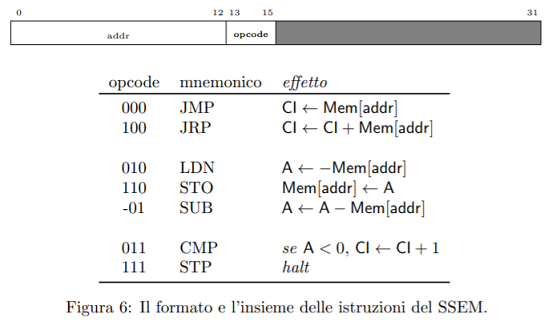
\includegraphics{images/1.png}
\end{center}
\subsection{Indipendenza dei dati} 
L'architettura scelta deve garantire l'\emph{indipendenza dei dati}. Questa consiste nella \underline{principale} proprietà del DBMS. Si permette a utenti e programmi applicativi che utilizzano una base di dati di interagire a un elevato livello di astrazione, che prescinde dai dettagli realizzativi utilizzati nella costruzione della base di dati. L'indipendenza dei dati si articola in
\begin{itemize}
	\item \textbf{indipendenza fisica}: si interagisce col DBMS in modo indipendente dalla struttura fisica dei dati. Posso modificare le strutture fisiche senza influire sulle descrizioni dei dati ad alto livello
	\item \textbf{indipendenza logica}: si interagisce col livello esterno della base in modo indipendente dal livello logico. Posso creare uno schema esterno in base a certe esigenze senza dover modificare lo schema logico. Inoltre, posso modificare il modello logico senza dover modificare le strutture esterne.
\end{itemize}
Fondamentalmente quanto detto rappresenta la differenza tra interfaccia e implementazione vista a \emph{Fondamenti di programmazione}.
\subsection{Vantaggi e svantaggi}
\subsubsection{Vantaggi}
\begin{itemize}
	\item Gestione centralizzata (e conseguente riduzione di ridondanze ed errori) con possibilità di “economia di scala”
	\item Disponibilità di servizi integrati per un'intera organizzazione (maggiore produttività)
	\item Indipendenza dei dati (favorisce lo sviluppo e la manutenzione delle applicazioni)
\end{itemize}
\subsubsection{Svantaggi} 
\begin{itemize}
	\item Costo dei prodotti e della transizione verso di essi
	\item Non scorporabilità (spesso) delle funzionalità (con riduzione di efficienza)
\end{itemize}
In certe circostanze può risultare utile, soprattutto quando lavoriamo in ambienti piccoli, ricorrere a un approccio più tradizionale nella conservazione dei dati.


\section{Concetto di \emph{transazione}}
Tutti i gestori attualmente in commercio sono detti \emph{transazionali} poichè basati su transazioni (forniscono meccanismi per definire ed eseguire transazioni).\\
La transazione consiste in un insieme di operazioni (di lettura e scrittura della memoria)
\begin{itemize}
	\item \textbf{indivisibili} (atomicità). Questo significa che se una delle operazioni non può essere eseguita allora la transazione nel suo complesso non può essere eseguita (Esempio: transazione bancaria, compio un prelievo da un conto A e un versamento in un conto B)
	\item \textbf{corrette} anche in presenza di concorrenza (controllo della concorrenza)
	\item \textbf{con effetti definitivi} (permanenza)
\end{itemize} Non possiamo vedere lo stato di questa sequenza, ma solo l'inizio e la fine: ciò che avviene nel mezzo non è detto sia corretto, l'importante è che al termine tutto sia effettivamente corretto.\\
Le transazioni possono essere molto complesse e in alcuni casi provocare errori: lo svolgimento di transazioni deve essere bloccato nel caso in cui possano emergere problemi. Il gestore, ogni volta, stabilisce se l'utente può effettivamente svolgere operazioni.\\
Quando la transazione termina con successo si ha un risultato di  tipo \emph{commit} (impegno) e quanto fatto viene salvato, altrimenti si ha un risultato di tipo \emph{aborted} (abortito) e non vengono apportate modifiche.
\section{Modello logico}
\paragraph{Perchè parliamo di modelli logici?} I programmi fanno riferimento ai dati, la cui struttura deve poter essere modificata senza modificare i programmi. Proprio per questo andiamo ad introdurre il \emph{modello logico}, un insieme di costrutti utilizzati per organizzare i dati. Un'organizzazione dei dati, distinta da quella dell'applicazione, permette di dividere l'interfaccia dall'implementazione con un approccio non diverso da quello visto con i moduli a \emph{Fondamenti}: il DBMS nasconde  l'implementazione e gli utenti si trovano in un livello astratto da cui possono compiere interrogazioni senza conoscere la struttura.
\paragraph{Esempio} Un esempio è il \emph{modello relazionale}, il cui costrutto caratterizzante è la relazione. Essa permette di definire insiemi di record omogeni a struttura fissa: una tabella.
\subsection{Schema e istanza}
Ogni tipo di dato nel modello logico è caratterizzato da
\begin{itemize}
	\item uno schema, sostanzialmente invariato nel tempo, che descrive la struttura
	\item un'istanza, i valori, che può variare rapidamente nel tempo.
\end{itemize}
Nel modello relazionale lo schema consiste nella prima riga della tabella, l'istanza nel corpo della stessa.
\section{Linguaggi per basi di dati}
Il linguaggio utilizzato permette la definizione degli schemi e la manipolazione delle tabelle. Si distinguono due tipi di linguaggio:
\begin{itemize}
	\item il \emph{Data definition language} (DDL) per la definizione di schemi
	\item il \emph{Data manipulation language} (DML) per l'interrogazione e l'aggiornamento
\end{itemize}
Alcuni linguaggi presentano entrambe le funzioni. Il più noto è l'SQL: è detto linguaggio testuale e interrattivo poichè un utente può scrivere l'interrogazione ed eseguirla immediatamente.
\subsection{Immersione in linguaggio ospite}
Caratteristica importante è la possibilità di "immergere" i comandi SQL in un linguaggio ospite: in Java, in C++, in PHP. Questo discorso è affrontato in un capitolo successivo.

\section{Architettura del DBMS}
Con architettura intendiamo il modello di esecuzione utilizzato da un sistema in cui esiste un DBMS. Tutte le realizzazioni di gestori utilizzano un'\emph{architettura distribuita}, caratterizzata dalla presenza di più macchine che lavorano autonomamente e interagiscono mediante la rete.
\subsection{Architettura a due livelli - \emph{client-server}}
L'architettura più diffusa è quella \emph{client-server}, detta anche \emph{a due livelli}. Abbiamo due macchine che comunicano attraverso la rete:
\begin{itemize}
	\item il server. Ha la base di dati e il DBMS, offre servizi e risponde alle richieste dei client.
	\item il client. Richiede servizi comunicando con il server attraverso la rete.
\end{itemize}
In alcune circostanze la macchina potrebbe fungere sia da server che da client, normalmente ciò non avviene. Il server deve avere la potenza sufficiente per svolgere tutte le operazioni richieste dai client in tempi accettabili. Ovviamente possono esserci più server e avere una base di dati distribuita.\\
Individuiamo due tipi di client:
\begin{itemize}
	\item \textbf{thin client} (il più diffuso): l'elaborazione dei dati (\emph{logica dell'applicazione}) avviene nel server. 
	\item \textbf{thick client}: l'elaborazione dei dati avviene nel client. Ciò può risultare svantaggioso: la macchina deve essere potente per trasmettere i dati a tutti i client e ognuna deve avere un rapporto fiduciario col gestore di dati. Inoltre non si possono avere più di poche centinaia di client.
\end{itemize}
\subsection{Architettura a tre livelli}
Con internet si passa a un'architettura \emph{a tre livelli}. Essa presenta:
\begin{itemize}
	\item un server contenente la base di dati
	\item un server applicativo che compie elaborazioni
	\item un client che compie interrogazioni
\end{itemize}
Anche in questo caso si possono avere più server, sia del primo tipo che del secondo. Il client, invia le richieste al server applicativo e questo dialoga con il server contenente la base di dati. 
\paragraph{Quale vantaggio si cela dietro questa struttura?} Il client è di tipo \emph{thin} e si occupa esclusivamente dell'interfacciamento (quindi possibile numero di client maggiore). In un certo senso il client coincide con il browser web! 
\paragraph{Sistemi eterogenei} Possiamo connettere sistemi non omogenei: posso compiere le solite domande che sono abituato a fare senza rendermi conto, per esempio, di avere un database di diverso tipo.
\section{Big Data}
Per definizione gli oggetti contenuti in base di dati sono di dimensioni enormi. Nel tempo abbiamo visto l'introduzione di strumenti informatici sempre più evoluti e l'aumento di produzione di dati. Descriviamo la cosa mediante le quattro v:
\begin{itemize}
	\item \textbf{Volume}: in un minuto si ottiene già una grande quantità di dati. Milioni di interrogazioni a Google, di like e share su Facebook, di downloads da youtube... 
	\item \textbf{Velocità}: i dati si muovono ad alta vellocità. Esistono tecniche che permettono di analizzare i flussi: non salvo i dati ma i risultati dell'analisi dei flussi.
	\item \textbf{Varietà}: i dati non sono più esclusivamente strutturati in tabella, ma prevalentemente non strutturati (testi, immagini, vocali, video)
	\item \textbf{Veridicità}: i dati estratti sono veritieri? Posso estrarre informazioni vere anche in presenza di gravi errori, imprecisioni e incompletezze. 
\end{itemize}
\paragraph{\emph{data science}} La qualità deve essere sempre garantita: ciò ha favorito la nascita della \emph{data science}, una branca dell'informatica che collabora con la matematica (in particolare con la statistica). La data science include i seguenti aspetti:
\begin{itemize}
	\item \emph{Data cleaning}: costruzione di una raccolta dati con un sufficiente livello di qualità
	\item \emph{Data integration}: costruzione di una raccolta dati integrata a partire da differenti sorgenti.
	\item \emph{Data mining}: estrazione di informazioni utili dai dati.
	\item \emph{Metodi predittivi} Metodi per prevedere mediante osservazioni nel passato dati riguardanti il futuro
	\item \emph{Machine learning}: metodo predittivo particolare. Vengono forniti alla macchina dei dati iniziali, che ne permettono l'educazione e una progressiva autonomia nell'analisi dei dati.
\end{itemize}
\paragraph{\emph{Data engineers}} Noi ingegneri ci occuperemo soprattutto delle infrastrutture per analizzare i dati (e non delle tecniche di analisi come il \emph{data scientist}).

\section{Sistemi non relazionali e potenziamento di un sistema} Negli ultimi anni sono emersi nuovi sistemi non relazionali in cui si rinuncia ad alcuni elementi citati fino ad ora per ottenere maggiore flessibilità. I sistemi NoSQL, per esempio, non hanno una vera e propria struttura dati: semplicemente mi limito ad aggiungere e rimuovere colonne quando necessario. Sia i dati che gli utenti tendono ad aumentare e quindi risulta necessario scalare. Posso adottare uno dei seguenti approcci:
\begin{itemize}
	\item scalare verticalmente, quindi adottare un approccio centralizzato e aumentare la potenza dei miei server (costi elevati)
	\item scalare orizzontalmente, approccio distribuito in cui posso aggiungere nuovi server standard e non potentissimi (economico)
\end{itemize} 
L'ultimo approccio è quello adottato con i database \emph{NoSQL}. Ho Mario Bianchi: ogni volta che ho informazioni nuove su di lui continuo ad aggiungerle. Ottengo delle liste. Questi sistemi sono utili in particolare quando abbiamo una crescita molto elevata, quasi incontrollata, di dati. La loro semplicità, tuttavia, è dovuta anche alla mancanza di controlli sull'integrità dei dati: il compito ricade sull'applicazione che dialoga col database.  Inoltre l'assenza di una vera e propria struttura dati rende difficile il passaggio a un altro tipo di database. Segue che questi database non domineranno mai il mercato.
\pagebreak

\section{Modello relazionale}
Il \emph{modello relazionale} si basa sul concetto matematico di relazione, con alcune differenze. Esso permette di definire insiemi di record omogeni a struttura fissa: una tabella.
\paragraph{Prodotto cartesiano}
Dati $n$ insiemi $D_1,\dots,D_n$ (che costituiscono i domini del prodotto cartesiano) non necessariamente distinti il prodotto cartesiano $D_1 \times \dots \times D_n$ consiste nell'insieme delle \emph{n-uple} ordinate $(v_1,\dots,v_n)$ dove $v_k \in D_k, k=1\dots n$. Il prodotto cartesiano può essere svolto anche tra insiemi che non presentano la stessa cardinalità.
\paragraph{Relazione matematica}
Una relazione matematica sugli insiemi $D_1,\dots,D_n$ consiste in un sottoinsieme del prodotto cartesiano $D_1 \times \dots \times D_n$ (quindi si considerano solo parte delle \emph{n-uple ordinate} effettivamente ottenute col prodotto cartesiano)
\paragraph{Grado del prodotto cartesiano}
Il grado del prodotto cartesiano consiste nel numero delle componenti di ogni \emph{n-upla} del prodotto cartesiano.
\paragraph{Cardinalità della relazione}
La cardinalità della relazione consiste nel numero delle \emph{n-uple} ottenute.

\noindent Si ha (nella matematica) una \emph{struttura posizionale} in cui la posizione consiste nell'indice del dominio. Si individua il ruolo di ciascun dominio a partire dalla posizione. L'ordine delle colonne ha un significato ben preciso, mentre l'ordine delle righe non ha importanza (non essendo numerate non si hanno n-uple, ma tuple).
\subsection{Passaggio a struttura non posizionale}
Se associamo ad ogni colonna, e quindi ad ogni dominio, un nome (che chiameremo \emph{attributo}), facciamo venir meno la notazione posizionale introdotta precedentemente: non ho più bisogno di conoscere la posizione ma semplicemente il nome associato agli elementi presenti in una colonna. Segue che non avrà importanza nè l'ordine delle colonne nè l'ordine delle righe.

\subsection{Tabella}
Le relazioni sono rappresentate attraverso tabelle. Si ha una relazione quando:
\begin{itemize}
	\item i valori di ogni colonna sono omogenei fra loro (quindi in una colonna avrò celle solo di un certo tipo: string, int...)
	\item le righe sono diverse fra loro (non ho doppioni)
	\item le intestazioni delle colonne sono diverse fra loro (non esistono più colonne con lo stesso attributo)
\end{itemize}
Possiamo stabilire un collegamento fra tabelle diverse mediante valori uguali in tuple diverse. Prendiamo per esempio una tabella \emph{Studenti} e una \emph{Esami}. Si stabilisce un collegamento mediante l'uguaglianza tra il campo \emph{matricola} presente in \emph{studenti} e il campo \emph{studente} presente in \emph{esami}!

\paragraph{Istanza} L'istanza è un insieme di tuple in cui si ha un valore per ogni attributo\footnote{Alle diapositive, 12,13 e 14 viene proposta un'alternativa basata su riferimenti espliciti gestiti dal sistema (puntatore). La cosa presenta dei vantaggi:indipendenza delle strutture fisiche e dati portabili più facilmente da un sistema ad un altro. L'utente finale, inoltre, vede gli stessi dati dei programmatori. I puntatori a livello fisico, tuttavia, non sono visibili a livello logico}.
\paragraph{Schema di relazione} uno schema di relazione è caratterizzato dalla presenza del nome e di un insieme di attributi. Solitamente presenta la forma $R(A_1,\dots,A_n)$ dove $R$ è il nome della relazione ed $A_1,\dots,A_n$ sono gli attributi.
\paragraph{Schema di base di dati} Insieme di schemi di relazione. Può essere introdotto mediante la seguente forma: $R = \{ R_1(X_1),\dots,R_k(X_k)\}$.
\paragraph{Tupla su un insieme di attributi} Una tupla su insieme di attributi $X$ è una funzione che associa a ciascun attributo $A$ in $X$ il valore del dominio di $A$. Il valore della tupla $t$ sull'attributo $A$ può essere denotato mediante la forma $t[A]$.
%\paragraph{Istanza di relazione su uno schema $R(X)$} Insieme $r$ di tuple su $X$
%\paragraph{Istanza di base di dati su uno schema $R = \{ R_1(X_1),\dots,R_n(X_n)\}$} Insieme di relazioni $r=\{r_1,\dots,r_n\}$ (con $r_i$ relazione su $R_i$)
\subsection{Informazione incompleta}
Il modello relazionale impone una struttura rigida per i dati: le tuple devono corrispondere agli schemi di relazione, ma potrebbe succedere che i dati disponibili non corrispondano al formato previsto. 
\paragraph{Necessità di un valore nullo} Introduciamo a tal proposito il valore $NULL$: di principio, ricordiamo, non esiste il vuoto ma un valore che denota il vuoto. Il NULL può essere utilizzato per denotare 
\begin{multicols}{3}
	\begin{itemize}
		\item valori sconosciuti; 
		\item valori inesistenti;
		\item valori non interessanti.
	\end{itemize}
\end{multicols} \noindent Il valore NULL si aggiunge a quelli parte del dominio di ciascun attributo. Segue che è necessario restringere la possibilità di inserimento di valori nulli in una relazione (in alcuni casi potrebbe essere necessario richiedere l'inserimento obbligatorio di un valore).
\paragraph{Esempio} Aggiunta di una persona all'interno di una tabella: tra gli attributi abbiamo il \emph{ruolo}, ma questa persona non ha ruoli o inizialmente non lo conosciamo. Grazie al valore NULL posso inserire delle tuple parziali aggiornabili successivamente.

\section{Vincoli di integrità}
Esistono istanze di basi di dati che pur essendo sintatticamente corrette non rappresentano informazioni possibili per il contesto. Il gestore, mediante una serie di proprietà (che esprimono la consistenza della base di dati), garantisce la qualità dei dati.
%\paragraph{Esempio 1} Prendiamo i voti universitari: 30 e lode è l'unico voto con lode accettabile. Il gestore, se riceve un voto diverso con lode, lo respinge segnalando un errore. Stessa cosa con i voti insufficienti: se inserisco un voto inferiore a 18 il gestore segnala errore.
%\paragraph{Esempio 2} Provo a inserire un voto a Mario Bianchi ma ricevo errore. Ho due opzioni: la matricola inserita è errata o Mario Bianchi ha già un voto associato alla materia interessata.\\

\begin{definizione}[Vincoli di integrità]I	vincoli corrispondono a proprietà del mondo reale modellato dalla base di dati e interessano tutte le istanze.
\end{definizione}
\noindent I vincoli di integrità
\begin{itemize}
	\item permettono una descrizione più accurata della realtà
	\item contribuiscono alla qualità dei dati
	\item sono utili nella progettazione
	\item sono usati dai DBMS nella esecuzione delle interrogazioni
\end{itemize}
I vincoli sono associati allo schema e si considerano corrette solo le istanze che soddisfano tutti i vincoli.
\begin{definizione}[Vincolo - definizione tecnica]
	Un vincolo è un predicato che associa ad ogni istanze della base di dati il valore vero o falso. Se il predicato vale vero la proprietà è soddisfatta. Si distinguono \textbf{vincoli intrarelazionali} da \textbf{vincoli interrelazionali}.
\end{definizione}
\subsection{Vincoli intrarelazionali}
Un vincolo intrarelazionale è il vincolo di tupla: esprimono condizioni sui valori di ciascuna tupla, indipendentemente dalle altre. Più nello specifico possiamo parlare di vincolo di dominio se la condizione riguarda un solo attributo all'interno di una tupla.
\paragraph{Esempio 1} Ho una relazione $studenti$. Ciascun studente è identificato in modo univoco dal codice di matricola: segue che nella tabella non potranno essere presenti più studenti con la stessa matricoli.
\paragraph{Esempio 2} La lode può essere assegnata solo se il voto è uguale a 30. Non posso farlo con altre valutazioni!
\paragraph{Esempio 3} Lo studente può ottenere solo voti sufficienti: segue che nella tabella $esami$ non potrò inserire un valutazione inferiore a 18.

\noindent In riferimento al primo esempio parleremo di \emph{identificatori di tupla}: non posso avere due tuple con lo stesso valore dell'attributo matricola. Questo attributo consiste in una \emph{chiave}!
\begin{definizione}[Chiave]
	La chiave è un attributo che permette di identificare in modo univoco le tuple di una relazione. Precisamente:
	\begin{itemize}
		\item Un insieme $K$ di attributi si dirà superchiave se date due tuple $t_1$ e $_2$ esse non sono distinte con $t_1[k]=t_2[k]$
		\item Lo stesso insieme sarà definito chiave se consiste in una \emph{superchiave minimale}. Ciò significa che all'interno di $K$ non si trovano altre superchiavi.
	\end{itemize}
	Prendiamo i seguenti esempi:
	\begin{itemize}
		\item L'insieme $\{Matricola\}$ è superchiave ed è anche chiave poichè ha un solo attributo e l'insieme vuoto non permette l'identificazione di tuple
		\item L'insieme $\{Cognome,Nome,Nascita\}$ è superchiave. Nessuno dei sottoinsiemi possibili è superchiave: Cognome e Nome, Cognome e Nascita, Nome e nascita. Segue che l'insieme è anche chiave poichè superchiave minimale.
		\item L'insieme $\{Matricola,Corso\}$ è superchiave ma non superchiave minimale: esiste un sottoinsieme proprio $\{Matricola\}$, che è superchiave minimale. Segue che il primo insieme non è chiave
		\item L'insieme $\{Nome,Corso\}$ non è superchiave perchè nella relazione possono comparire tuple uguali sia su nome che su corso.
	\end{itemize}
\end{definizione}

\subsubsection{A cosa servono le chiavi?}
Ogni relazione contiene tuple distinte tra loro (definizione, è un insieme). Ogni relazione ha come superchiave l'insieme degli attributi su cui è definita, cioè ha almeno una chiave. L'esistenza della chiave permette di identificare in modo univoco ogni tupla garantendo l'accesso ad essa; è altrettanto utile per stabilire correlazioni fra dati di relazioni diverse. 
\paragraph{Valori nulli} Non è vietato che un attributo chiave assuma valori nulli, ma è sconsigliato generalmente. Presupponimo di avere una solo attributo chiave per identificare le tuple: in quel caso la chiave non può assumere valore nullo, altrimenti non potrei identificarla. Una chiave che non può assumere valori nulli è detta \textbf{chiave primaria} (rappresentata con sottolineatura).


\subsection{Vincoli interrelazionali}
Possiamo stabilire correlazioni tra relazioni diverse a partire dai valori delle \textbf{chiavi primarie}, in modo da mantenere la consistenza di una relazione in caso di modifica di un'altra.
\paragraph{Esempio} Abbiamo una seconda relazione $esami$. Tra gli attributi si ha la matricola identificativa dello studente: non devo poter inserire esami con matricole inesistenti o con matricole esistenti se l'esame è già stato svolto. Ciò vale non solo con l'aggiunta di nuovi esami ma anche in caso di modifica di esami precedenti. Si richiede di intervenire anche quando lo studente viene eliminato (dove vanno a finire le tuple dei suoi esami?)
\subsubsection{Vincolo di integrità referenziale}
\begin{definizione}[Vincolo di integrità referenziale]
	Un vincolo di integrità referenziale fra gli attributi $X$ di una relazione $R_1$ impone ai valori su $X$ in $R_1$ di comparire come valori della chiave primaria di $R_2$.
\end{definizione}
\paragraph{Integrità referenziali e valori nulli} In presenza di valori nulli posso ricorrere a vincoli meno restrittivi. La definizione precedente è valida, semplicemente si impone quanto detto ai valori $X$ diversi da NULL.
\subsection{Violazioni e interferenze}
\begin{itemize}
	\item Nel caso di violazione di vincoli intrarelazionali si rifiuta l'operazione.
	\item Nel caso di vincoli interrelazionali si parla di operazioni interferenti che determinano violazioni dei vincoli stabiliti. Abbiamo
	\begin{itemize}
		\item modifiche di valori (esempio modificare la matricola associata a un esame). L'operazione viene impedita
		\item azioni sulla tabella \emph{master}: eliminazione di una tupla o modifica dell'attributo riferito. Posso stabilire:
		\begin{itemize}
			\item l'eliminazione/modificata in cascata delle righe coinvolte;
			\item posso porre a NULL il valore dell'attributo referente (nelle tuple rimaste "orfane");
			\item assegnare un valore di default all'attributo referente;
			\item non consentire la cancellazione.
		\end{itemize}
	\end{itemize}
\end{itemize}
	\chapter{Mercoledì 11/03/2020}
\section{Interrogazioni}
L'interrogazione è un'operazione di lettura che non modifica la base di dati. In certe circostanze un'interrogazione può coinvolgere più tabelle! Abbiamo due tipi di semantiche:
\begin{itemize}
	\item \textbf{dichiarativa}, in cui si esprimono le proprietà del risultato. Essa ricorre al \emph{calcolo relazionale} e consiste nell'effettiva semantica del linguaggio! Le interrogazioni sono espresse ad alto livello.
	\item \textbf{operazionale}, si specificano le modalità di calcolo adottate dal gestore della base di dati per ottenere il risultato. In questo caso si ricorre all'\emph{algebra relazionale}. Poichè si parla di modalità di calcolo possiamo individuare i costi per l'esecuzione di una certa interrogazione
\end{itemize}
\subsection{\emph{query processor}} All'interno del gestore abbiamo un modulo detto \emph{query processor}, dove è definito il processo di esecuzione delle interrogazioni. Ciò permette al gestore di definire una strategia di esecuzione ottimale. Si hanno tre fasi:
\begin{itemize}
	\item \textbf{Analisi lessicale, sintattica e semantica} della query scritta: si ottiene una corrispondente espressione algebrica;
	\item \textbf{Ottimizzazione algebrica} dell'espressione: si ottiene una nuova espressione algebrica attraverso ottimizzazioni valide in ogni caso (Esempio: \emph{push selections down} e \emph{push projections down})
	\item \textbf{Ottimizzazione basata sui costi}: sfruttando quanto contenuto nel cosiddetto \emph{catalogo}, cioè informazioni quantitative (\emph{profili}) riguardanti il database (numero di tuple, dimensione della tupla o dei valori, numero di valori distinti, valori minimi e massimi degli attributi...), possiamo stimare la dimensione dei risultati intermedi ed effettuare ulteriori ottimizzazioni (riparleremo di questa ottimizzazione nell'ultima lezione).
\end{itemize}

\subsubsection{Ottimizzazione algebrica}
Le due fasi di ottimizzazione si basano sull'euristica: sulla base dei dati a disposizione decidiamo quali procedure adottare per eseguire un'istruzione. Parlare di "euristica", tuttavia, è un po' improprio: il processo si basa soprattutto sulla nozione di equivalenza.
\paragraph{Equivalenza} Due espressioni sono equivalenti se producono lo stesso risultato!
\pagebreak

\section{Algebra relazionale}
Nell'algebra relazionale abbiamo operatori applicati su una o più relazioni. Gli operatori producono nuove relazioni e possono essere composti. Analizzeremo \textbf{operatori su insiemi} (unione, intersezione e differenza) ed \textbf{operatori su relazioni} (ridenominazione, selezione, proiezione, join). I primi operatori sono applicati a relazioni che presentano gli stessi attributi: la relazione prodotta avrà gli stessi attributi. I secondi, ad eccezione del join (il più complesso tra quelli che vedremo), sono monadici.\\

\noindent Nelle successive definizioni considereremo $X$ come l'insieme degli attributi.
\subsection{Unione ($r_1 \cup r_2$)}
Date due relazioni $r_1(X), r_2(X)$, l'unione $r_1(X) \cup r_2(X)$ consiste in una nuova relazione che contiene sia le tuple di $r_1$ che quelle di $r_2$.
\paragraph{Esempio dalle diapositive} Abbiamo le relazioni $\mathbf{laureati\_triennal}i$ e $\mathbf{laureati\_magistrali}$.\\
Ottengo una nuova relazione che elenca le persone che hanno conseguito almeno una laurea. Nei risultati della nuova relazione vediamo Neri e Verdi che hanno conseguito sia la laurea triennale che quella magistrale, un altro Neri che ha solo la laurea magistrale, Rossi che ha solo la laurea triennale.

\begin{center}
	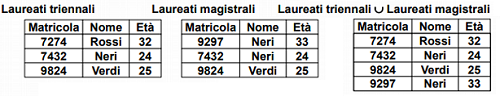
\includegraphics{images/28.PNG}
\end{center}

\subsection{Intersezione ($r_1 \cap r_2$)}
Date due relazioni $r_1(X), r_2(X)$, l'intersezione $r_1(X) \cap r_2(X)$ consiste in una nuova relazione che contiene solo le tuple appartenenti ad entrambe le relazioni.
\paragraph{Esempio dalle diapositive} Prendiamo lo stesso esempio di prima. Ottengo una nuova relazione che elenca le persone che hanno preso sia la laurea magistrale che quella triennale. Gli unici che hanno conseguito entrambe le lauree sono Neri e Verdi: nell'istanza avrò soltanto le loro tuple.
\begin{center}
	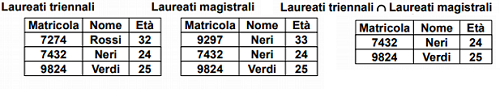
\includegraphics{images/29.PNG}
\end{center}
\pagebreak
\subsection{Differenza ($r_1 - r_2$)}
Date due relazioni $r_1(X), r_2(X)$, la differenza $r_1(X)-r_2(X)$ consiste in una nuova relazione che contiene le tuple di $r_1$ che non appartengono anche ad $r_2$. L'operatore è rappresentato dal segno meno.
\paragraph{Esempio dalle diapositive} Idem con patate. Ottengo una relazione in cui si hanno gli elementi di $\mathbf{laureati\_triennali}$ non presenti in $\mathbf{laureati\_magistrali}$, cioè coloro che hanno conseguito la laurea triennale ma non quella magistrale.\\Nella prima relazione abbiamo Rossi, Neri e Verdi: osserviamo che Neri e Verdi sono presenti anche nella seconda relazione. Segue che l'unica tupla presente nell'istanza sarà quella di Rossi.

\begin{center}
	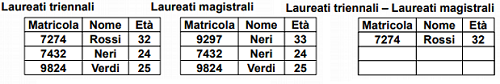
\includegraphics{images/30.PNG}
\end{center}

\subsection{Ridenominazione ($\rho_{a_1,\dots,a_n \leftarrow b_1,\dots,b_n}$)}
L'operatore monadico di ridenominazione ci permette di modificare lo schema di una relazione alterando gli attributi. Questa cosa ci permetterà di applicare gli operatori di insieme a relazioni che hanno schema simile ma non equivalente.
\paragraph{Esempio dalle diapositive} Abbiamo le relazioni $\mathbf{paternita}(padre,figlio)$ e $\mathbf{maternita}(madre,figlio)$ a cui voglio applicare l'operatore unione. Essi hanno schema simile, ma un attributo diverso. Mediante l'operatore di ridenominazione modifico l'attributo \emph{padre} in \emph{genitore}. Faccio la stessa cosa con \emph{madre}. A questo punto posso applico l'operatore di insieme.

\begin{center}
	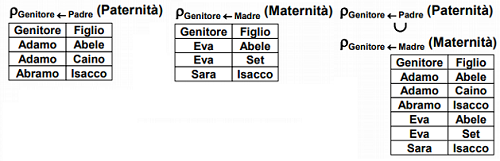
\includegraphics{images/31.PNG}
\end{center}

\subsection{Selezione ($\sigma_F$) - decomposizione orizzontale}
L'operatore monadico di selezione restituisce una nuova relazione con lo stesso schema ma con solo una parte delle tuple. Viene mostrato un sottoinsieme i cui elementi sono determinati a partire da un'espressione booleana $F$: se l'espressione è vera la tupla è considerata appartenente alla nuova relazione, altrimenti viene esclusa.
\paragraph{Esempio dalle diapositive} Ho una relazione $\mathbf{Impiegati}(matricola,cognome,filiale,stipendio,eta)$. Voglio mostrare soltanto gli impiegati con uno stipendio superiore ai 50.000 euro. Posso rendere la cosa più articolata mostrando soltanto gli impiegati che soddisfano la condizione precedente e che lavorano nella filiale di Milano.

\begin{center}
	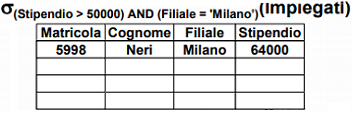
\includegraphics{images/32.PNG}
\end{center}

\paragraph{Attenzione ai valori nulli} Prendiamo la stessa relazione e consideriamo le persone con $eta > 40$. Le tuple con età nulla vengono automaticamente escluse: ciò può essere evitato indicando che il valore può essere anche nullo (Ho le forme \emph{IS NULL} e \emph{IS NOT NULL}). 
\[\sigma_{Eta > 40}(Impiegati)\;\;\;\;\;\sigma_{(Eta > 40)\, OR \;(Eta\; \mathbf{IS\;NULL})}(Impiegati)\]
\subsection{Proiezione ($\pi_Y$) - decomposizione verticale}
L'operatore monadico di proiezione restituisce una nuova relazione che contiene un insieme di tuple ristrette agli attributi Y (ho un sottoinsieme degli attributi, fondamentalmente).
\paragraph{Esempio dalle diapositive} Riprendiamo l'esempio utilizzato negli operatori di insieme: creo una nuova relazione in cui mostro soltanto matricole e cognomi.

\begin{center}
	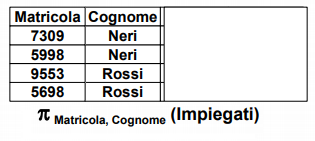
\includegraphics{images/33.PNG}
\end{center}

\paragraph{Cardinalità delle proiezioni} Può capitare che una proiezione produca una relazione con un numero inferiore di tuple. Ciò può avvenire escludendo la chiave \emph{matricola}. Osserviamo che sono presenti nella relazione iniziale due Neri e due Rossi. Nella relazione finale ho due Neri e un \emph{solo} Rossi poichè abbiamo ignorato l'attributo che identifica le tuple in modo univoco: si osserva, inoltre, che entrambi i Rossi lavorano nella filiale di Roma.

\begin{center}
	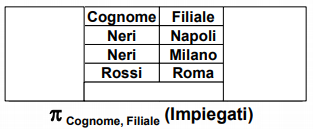
\includegraphics{images/34.PNG}
\end{center}

% Nelle due relazioni hanno la stessa età. Si osserva che nell'unione l'identità delle due relazioni viene persa e conseguentemente nella nuova relazione non si hanno duplicati: essa conterrà semplicemente le persone che si sono laureate almeno una volta.
\subsection{Composizione degli operatori}
Come già detto posso creare una composizione di operatori: per esempio posso unire l'operatore selezione con l'operatore proiezione. Nella composizione è necessario porre attenzione all'ordine degli operatori: un ordine diverso può portare a risultati diversi.

\begin{center}
	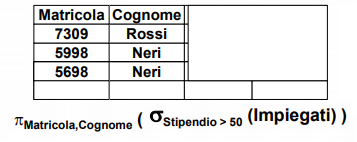
\includegraphics{images/35.PNG}
\end{center}
Adesso spingiamoci oltre: con gli operatori introdotti fino ad ora non possiamo correlare relazioni profondamente diverse tra loro!
\subsection{Operatore Join}
Con l'operatore JOIN ossiamo correlare dati appartenenti a relazione diverse!
\subsubsection{Prodotto cartesiano ($r_1 \times r_2$)}
Operatore binario, di fatto il più costoso per il DBMS. Abbiamo due relazioni: combiniamo le tuple di $r_1$ con le tuple di $r_2$. Ottengo una nuova relazione dove
\begin{itemize}
	\item lo schema consiste nell'unione degli attributi delle due relazioni
	\item l'istanza è caratterizzata da tuple ottenute mediante il prodotto cartesiano matematico.
\end{itemize}
\begin{center}
	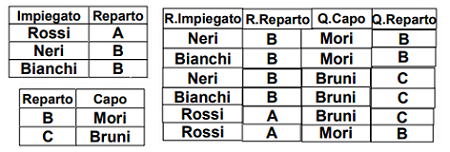
\includegraphics{images/38.PNG}
\end{center}
\subsubsection{Join naturale ($r_1 \Join r_2$)}
Il \emph{join naturale} è un operatore binario che restituisce una relazione con schema uguale all'unione degli attributi degli schemi di $r_1(X_1)$ e $r_2(X_2)$ ($X_1 \cup X_2$). Si individua che 
\[r_1 \Join r_2=\{t \in X_1 \cup X_2\;|\; t[X_1] \in r_1, t[X_2] \in r_2\}\]
Il join naturale consiste in un insieme di tuple da cui ottengo tuple appartenenti alla relazione $r_1$ se applico una proiezione limitata a $X_1$ e tuple appartenenti alla relazione $r_2$ se applico una proiezione limitata a $X_2$.
Abbiamo due situazioni:
\begin{itemize}
	\item \textbf{presenza di attributi con lo stesso nome}: le tuple vengono costituite se il valore degli attributi comuni è uguale
	\item \textbf{senza attributi con nome comune}: quello che si ottiene equivale al prodotto cartesiano. Ho un numero di tuple pari al prodotto delle cardinalità degli operandi (le tuple sono tutte combinabili)
\end{itemize}
\paragraph{Osservazione} Solitamente non è possibile tornare alle relazioni originali dopo aver applicato il join.
\paragraph{Esempio dalle diapositive} Riprendiamo le relazioni $impiegati$ e $caporeparti$. Rossi non è tra le tuple poichè non è combinabile con nessun capo reparto. Si osserva che il capo del reparto C non può essere combinato con nessun impiegato (non si hanno impiegati al reparto C). 
\begin{center}
	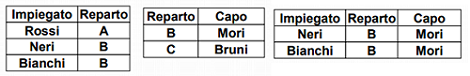
\includegraphics{images/36.PNG}
\end{center}
Potrebbe succedere che per un reparto (il B in questo caso) si abbiano due capireparto: Neri e Bianchi (del reparto B) vengono combinati due volte!
\begin{center}
	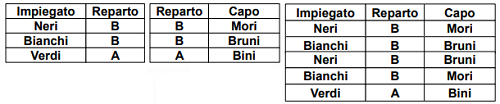
\includegraphics{images/37.PNG}
\end{center}
\paragraph{Esempio senza attributi comuni}
\begin{center}
	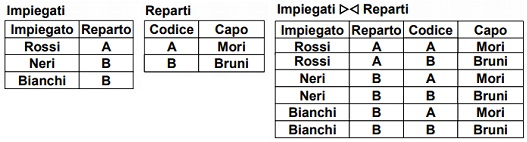
\includegraphics{images/39.PNG}
\end{center}
\paragraph{In generale}
\begin{itemize}
	\item Date due relazioni $R_1(X_1),R_2(X_2)$ si osserva che la proiezione di $X_1$ del join naturale tra $R_1$ e $R_2$ è inclusa in $R_1$.
	\[\pi_{X_1}(R_1\Join R_2) \subseteq R_1\]
	Se non si hanno attributi comuni avviene il prodotto cartesiano e il risultato dell'espressione coincide con $R_1$. Se si hanno attributi comuni il risultato non coincide con il prodotto cartesiano e due tuple vengono associate solo se si hanno le condizioni. Segue che il non-JOIN di alcune tabelle potrebbe comportarmi l'esclusione di alcune tuple di $R_1$ e quindi avere come risultato un sottoinsieme di $R_1$.
	\item Data una relazione $R(X)$, dove $X=X_1 \cup X_2$, il join naturale tra la proiezione di $X_1$ di $R$ e la proiezione di $X_2$ di $R$ contiene $R$
	\[(\pi_{X_1}(R))\Join(\pi_{X_2}(R))\supseteq R\]
	Se non si hanno attributi comuni tra $X_1$ e $X_2$ segue un prodotto cartesiano che mi porta ad avere un numero di tuple maggiore rispetto a prima. Ho quindi un insieme più grande che contiene l'insieme $R$ iniziale. Se ho attributi comuni tra $X_1$ e $X_2$ allora può esserci la possibilità che il risultato sia uguale ad $R$ originario.
\end{itemize}
\subsubsection{\emph{theta-join} (spesso \emph{equi-join})}
Posso ridurre il prodotto cartesiano attraverso una relazione del tipo $\sigma_F(R_1 \times R_2)$. La stessa operazione può essere fatta attraverso un operatore derivato detto \emph{theta-join}: prendo soltanto le tuple che fanno JOIN e che soddisfano delle condizioni.
\[R_1 \Join_F R_2\]
La condizione $F$ è spesso una congiunzioni di atomi di confronto caratterizzati da un operatore di confronto e attributi di relazioni diverse. Se l'operatore di confronto è l'uguale allora si ha l'\emph{equi-join}. \\
Riprendiamo l'esempio di prima dove non si hanno attributi comuni. Svolgiamo l'equi-join stabilendo un legame valido tra tuple se Reparto=Codice.
\begin{center}
	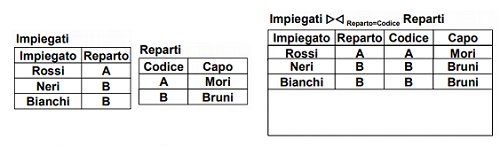
\includegraphics{images/40.PNG}
\end{center}
\subsection{JOIN operatore non primitivo}
\begin{center}
	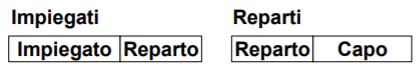
\includegraphics{images/75.PNG}
\end{center}
Il Join non è un operatore primitivo (diciamo, un "prodotto cartesiano schietto"). Individuiamo che
\paragraph{Relazione tra JOIN Naturale e prodotto cartesiano}
\[Impiegati \Join Reparti = \pi_{Impiegato,Reparto,Capo}(\sigma_{I.reparto=reparto}(\rho_{I.reparto \leftarrow Reparto}(Impiegati) \times Reparti))\]
\begin{itemize}
	\item Applico la ridenominazione alla relazione \emph{Impiegati} per poter usare la selezione
	\item Eseguo il prodotto cartesiano tra la relazione $\rho_{I.Reparto\leftarrow Reparto}(Impiegati)$ e \emph{Reparti}. 
	\item Applico la selezione, scegliendo i record che soddisfano la condizione $I.Reparto=Reparto$
	\item Proietto gli attributi $Impiegato, Reparto, Capo$. $I.Reparto$ ha lo stesso valore di $Reparto$, non serve proiettarlo nuovamente.
\end{itemize}
\paragraph{Relazione tra JOIN Naturale ed equi-join}
\[Impiegati \Join Reparti = \pi_{Impiegato,Reparto,Capo}(\rho_{I.reparto \leftarrow Reparto}(Impiegati) \Join_{I.Reparto=Reparto} Reparti)\]
\begin{itemize}
	\item Applico la ridenominazione alla relazione \emph{Impiegati} per poter usare la selezione
	\item Eseguo l'equi-JOIN tra la relazione $\rho_{I.Reparto\leftarrow Reparto}(Impiegati)$ e \emph{Reparti}, scegliendo soltanto le combinazioni di record che soddisfano l'uguaglianza $I.Reparto=Reparto$
	\item Proietto gli attributi $Impiegato, Reparto, Capo$. $I.Reparto$ ha lo stesso valore di $Reparto$, non serve proiettarlo nuovamente.
\end{itemize}
\subsection{Equivalenza di espressioni}
Due espressioni sono equivalenti se producono lo stesso risultato qualunque sia l'istanza attuale della base di dati. L'equivalenza è un concetto importante poichè i DBMS, molto spesso, eseguono espressioni equivalenti a quelle date, meno costose. Vediamo due esempi di euristica fondamentale in cui si applica uno dei principi base dell'ottimizzazione: esecuzione di selezioni e proiezioni il più presto possibile per ridurre la dimensioni dei risultati intermedi (e quindi il costo dell'operazione)
\subsubsection{\emph{Pushing selections down}}
Dato un attributo $A$ di $R_2$, che è attributo di interesse, individuo che
\[\sigma_{A=10}(R_1 \Join R_2)=R_1 \Join \sigma_{A=10}(R_2)\]
Le condizioni della selezione riguardano un attributo di $R_2$: eseguo la selezione prima di fare JOIN.
\subsubsection{\emph{Pushing projections down}}
Date due relazioni $R_1(X_1)$ e $R_2(X_2)$ con $Y_2 \subseteq X_2$, individuo che
\[\pi_{X_1\,Y_2}(R_1 \Join R_2)=R_1 \Join \pi_{Y_2}(R_2)\]
Proietto solo una parte degli attributi di $X_2$: eseguo la proiezione prima di fare JOIN.
\subsection{Procedura euristica dell'ottimizzatore}
\begin{itemize}
	\item Decomporre le selezioni congiuntive in successive selezioni atomiche
	\item Anticipare il più possibile le selezioni
	\item In una sequenza di selezioni anticipare le più selettive
	\item Combinare prodotti cartesiani e selezioni per formare JOIN
	\item Anticipare il più possibile le proiezioni (anche introducendone di nuove)
\end{itemize}
\subsection{Alberi per la rappresentazione di interrogazioni}
Possiamo utilizzare gli alberi per rappresentare le nostre interrogazioni: le foglie consistono nei dati (relazioni, file), i nodi intermedi negli operatori applicati.
\begin{center}
	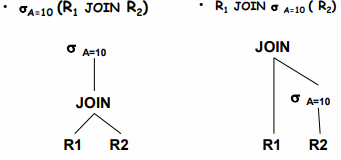
\includegraphics{images/48.PNG}
\end{center}
	\chapter{Mercoledì 18/03/2020}
La scorsa volta abbiamo intodotto l'algebra relazionale per spiegare le procedure adottate dal DBMS per eseguire le nostre interrogazioni. Adesso analizzeremo la semantica effettiva del linguaggio: il calcolo relazionale. Sappiamo che in SQL non è necessario scrivere una query già ottimizzata: possiamo scrivere versioni meno efficienti che saranno sottoposte a un processo di ottimizzazione.

\section{Calcolo relazionale}
\noindent Con \textbf{calcolo relazionale} intendiamo una famiglia di linguaggi dichiarativi che permette di specificare le proprietà del risultato di una certa interrogazione. Ne abbiamo due versioni:
\begin{itemize}
	\item il calcolo relazionale \textbf{applicato ai domini} (che presenta in modo naturale le proprietà dei predicati)
	\item il calcolo \textbf{su tuple con dichiarazioni di range} (versione adottata da SQL)
\end{itemize}

\subsection{Calcolo su domini}
\[\{A_1: x_1, \dots, A_n : x_n | f \}\]
\begin{itemize}
	\item $A_1,\dots,A_n$ sono nomi di attributi, $x_1,\dots,x_n$ sono nomi di variabili
	\item La lista delle coppie $A_i:x_i$ è detta \emph{target list} e definisce la struttura del risultato
	\item $f$ è una formula. Al suo interno possiamo porre:
	\begin{itemize}
		\item $R(A_1:x_1,\dots,A_n:x_n)$, dove $R(A_1\dots A_n)$ è uno schema di relazione $x_1\dots x_n$ sono variabili. Vera sui valori $x_1,\dots,x_n$ che formano una tupla della relazione r sullo schema R, nell'istanza di base di dati a cui l'espressione viene applicata.
		\item $x\theta y$, $x\theta c$: $x,y$ sono variabili, $c\;$ è una costante e $\theta$ è un operatore di confronto ($=, \neq, \leq, \geq, >, <$). Vera sui valori $x,y,c$ che soddisfano il confronto con operatore $\theta$.
		\item quantificatori nella forma
		\[\exists x (f)\;\;\;\,\forall x (f)\]
		Cioè: \textit{Esiste almeno una variabile $x$ che soddisfa la formula $f$}
	\end{itemize}
	Se $f_1$ e $f_2$ sono formule allora lo sono anche $\neg f_1$, $\neg f_2$, $f_1 \land f_2$, $f_1 \lor f_2$.
\end{itemize}
\subsection{Calcolo su tuple con dichiarazione di range}
\[\{x_1.Z_1,\dots,x_n.Z_n | x_i(R_1),\dots,x_j(R_m) | f \}\]
\begin{itemize}
	\item $x_1.Z_1,\dots,x_n.Z_n$ è la \emph{target list} (con $x_i$ nome di tupla e $Z_j$ insieme di nomi di attributi)
	\item $x_i(R_1),\dots,x_j(R_m)$ è la \emph{range list} (campo di variabilità delle variabili)
	\item $f$ è una formula. Al suo interno possiamo porre:
	\begin{itemize}
		\item formule atomiche del tipo $x_i.Z_i \, \theta \, x_j.Z_j$ o $x_i.Z_i \, \theta \, c$ (dove $c$ è una costante).
		\item connettivi come nel calcolo su domini
		\item quantificatori nella seguente forma
		\[\exists x (R)(f)\;\;\;\;\;\forall x (R)(f)\]
		\small
		Cioè: \textit{Esiste nella relazione $R$ almeno una variabile $x$ che soddisfa la formula $f$}
		\normalsize
	\end{itemize}
\end{itemize}

\subsection{Quantificatori esistenziali e universali}
All'interno dei predicati possiamo introdurre i cosiddetti \emph{quantificatori}. Abbiamo il quantificatore esistenziale $\exists$ e quello universale $\forall$. I due sono intercambiabili, nel senso che ne basta uno per esprimere qualunque cosa. Le \emph{leggi di de Morgan} valgono, \emph{mutatis mutandis}, anche per i quantificatori:
\begin{itemize}
	\item $\exists x(f) = \neg(\forall x(\neg(f)))$
	\item $\forall x(f)=\neg(\exists x(\neg(f)))$
\end{itemize}
\paragraph{Ricordiamo le leggi di De Morgan, già viste a \emph{Fondamenti di programmazione}}
\[\boxed{\neg(f \land g)=\neg(f) \lor \neg(g)}\;\;\;\;\;\;\;\;\;\;\;\,\;\boxed{\neg(f\lor g) = \neg(f) \land \neg(g)}\]
Date due condizioni $f$ e $g$:
\begin{enumerate}
	\item La negazione dell'AND si ha quando almeno una delle condizioni è negata
	\item La negazione dell'OR si ha quando entrambe le condizioni sono negate
\end{enumerate}
\paragraph{Quando sono necessari?} I quantificatori possono essere omessi in certe circostanze, ma in altre sono obbligatori: parliamo di interrogazioni più complesse come, per esempio, la differenza.  

\subsection{Esempi}\paragraph{Base di dati per gli esempi}
\begin{Verbatim}[commandchars=+\[\]]
	IMPIEGATI(+underline[Matricola], Nome, Età, Stipendio)
	SUPERVISIONE(+underline[Capo, Impiegato])
\end{Verbatim}
\paragraph{Trovare gli impiegati che guadagnano più di 40 milioni} 
\begin{itemize}
	\item \textbf{Su domini}: \{ Matricola: m, Nome : n, Età: e, Stipendio: s $|$ Impiegati(Matricola: m, Nome: n, Età: e, Stipendio: s) $\land$ s $>$ 40 \}
	\item \textbf{Su tuple con dichiarazione di range}: \{i.* $|$ i(Impiegati) $|$ i.Stipendio $>$ 40\}
\end{itemize}
\paragraph{Trovare nome e matricola degli impiegati che guadagnano più di 40 milioni} 
\begin{itemize}
	\item \textbf{Su domini}: \{ Matricola: m, Nome: n $|$ Impiegati(Matricola: m, Nome: n, Età: e, Stipendio: s) $\land$ s $>$ 40\}
	\item \textbf{Su tuple con dichiarazione di range}: \{ i.(Matricola, Nome) $|$ i(Impiegati) $|$ i.Stipendio $>$ 40 \}
\end{itemize}
\paragraph{Trovare matricola e nome dei capi i cui impiegati guadagnano tutti più di 40 milioni}
\begin{itemize}
	\item \textbf{Primo metodo con calcolo sui domini}: \{ Matricola: c, Nome: n $|$ Impiegati(Matricola: c, Nome: n, Età: e, Stipendio: s) $\land$ $\forall m'(\forall n' (\forall e' ( \forall s'(Impiegati$(Matricola: m', Nome: n', Età: e', Stipendio: s'\} $\land$ Supervisione(Capo:c, Impiegato:m') $\land$ s' $>$ 40))))\}
	\item \textbf{Secondo metodo con calcolo sui domini}: \{ Matricola: c, Nome: n $|$ Impiegati(Matricola: c, Nome: n, Età: e, Stipendio: s) $\land$ $\neg(\exists m'(\exists n' (\exists e' ( \exists s'(Impiegati$(Matricola: m', Nome: n', Età: e', Stipendio: s'\} $\land$ Supervisione(Capo:c, Impiegato:m') $\land$ s' $\leq$ 40)))))\}
	\item \textbf{Terzo metodo con calcolo su tuple}: \{i.(Matricola, Nome) $|$ s(Supervisione), i(Impiegati) $|$ i.Matricola = s.Capo $\land$ $\neg(\exists i$(Impiegati)(s.Impiegato=i.Matricola $\land$ i.Stipendio $\leq$ 40)))\}
\end{itemize}
\subsection{Discussione sul calcolo su domini}
Il calcolo su domini è dichiarativo, ma eccessivamente verboso con possibilità di scrivere espressioni sensa senso dipendenti dal dominio e aventi risultati di grandi dimensione. Nell'algebra, invece, tutte le espressioni hanno un senso e sono indipendenti dal dominio.
\paragraph{Indipendenza dal dominio} Un'espressione si dice indipendente dal dominio se il suo risultato, su ciascuna istanza di base di dati, non varia al variare del dominio rispetto al quale l'espressione è valutata.
\paragraph{Esempio di espressione dipendente dal dominio} Un esempio di espressione dipendente dal dominio è la seguente:
\[\{ A_1 : x_1, A_2 : x_2\;|\;R(A_1 : x_1, A_2 : x_2) \land x_2 = x_2 \}\]
$x_2 = x_2$ è una condizione sempre vera: se il dominio include gli interi da $0$ a $99$ avremo 100 tuple, se invece il dominio va da $0$ a $999$ avremo 1000 tuple!
\subsection{Discussione sul calcolo su tuple}
Le variabili rappresentano tuple e si ha minore verbosità. Alcune interrogazioni importanti non possono essere espresse, in particolare le unioni:
\[R_1(AB) \cup R_2(AB)\]
Ogni variabile nel risultato ha un solo range, mentre vorremmo tuple sia della prima relazione che della seconda. Intersezione e differenza, comunque sia, sono esprimibili. Per questa motivazione SQL prevede esplicitamente un operatore unione, ma non tutte le versioni prevedono intersezione e differenza.
\subsection{Calcolo e algebra relazionale}
Calcolo e algebra relazionale sono ''equivalenti'':
\begin{itemize}
	\item Per ogni espressione del calcolo relazionale che sia indipendente dal dominio esiste un'espressione dell'algebra relazionale equivalente a essa
	\item Per ogni espressione dell'algebra relazionale esiste un'espressione del calcolo relazionale equivalente a essa (e di conseguenza indipendente dal dominio)
\end{itemize}
Possono espresse buona parte delle interrogazioni, però ci sono cose non esprimibili come la \emph{chiusura transitiva}.
\subsection{Chiusura transitiva di una relazione}
La chiusura transitiva non può essere definita poichè dovrei fare il JOIN innumerevoli volte per arrivare al risultato, alla tabella definitiva.
\paragraph{Esempio} Consideriamo la seguente relazione
\begin{Verbatim}[commandchars=+\[\]]
	Supervisione(+underline[Impiegato, Capo])
\end{Verbatim}
Voglio trovare, per ogni impiegato, tutti i superiori (cioè il capo, il capo del capo, e così via). Nel seguente esempio (teniamo conto che vi è la ridenominazione dell'attributo \emph{Campo}) la cosa pare semplice
\begin{center}
	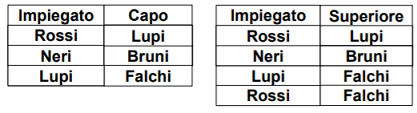
\includegraphics{images/140.PNG}
\end{center}
ma se abbiamo una nuova n-upla come nel secondo esempio risulta necessario stabilire ulteriori legami. Se il capo di Rossi è Lupi e il capo di Lupi è Falchi allora il capo di Rossi è Falchi.
\begin{center}
	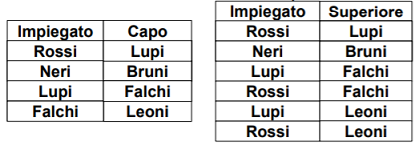
\includegraphics{images/141.PNG}
\end{center}
\paragraph{Conclusione} Non possiamo calcolare la chiusura transitiva di una relazione qualunque. In algebra relazionale l'operazione si simulerebbe con un numero di JOIN illimitato.

\section{Estensione dell'algebra relazionale}
Il modello relazionale può essere facilmente estesso a comprendere operatori SQL non direttamente riconducibili agli operatori algebrici introdotti. Ciò non comporta una modifica del modello.
\subsection{JOIN Esterno}
Ho tre tipi di OUTER JOIN: left, right e full. Questi permettono di combinare tuple che normalmente non fanno JOIN.
\begin{itemize}
	\item Il LEFT JOIN: mantiene tutte le tuple della prima relazione
	\item Il RIGHT OUTER JOIN: mantiene tutte le tuple della seconda relazione
	\item Il FULL OUTER JOIN: mantiene tutte le tuple
\end{itemize}
\paragraph{Esempio di JOIN} \emph{Trovare la matricola dei capi degli impiegati che guadagnano tutti più di 40.000 euro}
\begin{center}
	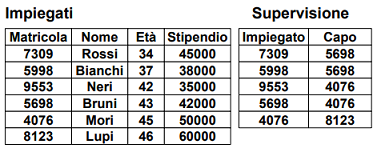
\includegraphics{images/60.PNG}
\end{center}
Si individuano impiegati non subordinati a nessuno, cioè i capi stessi. Con un JOIN normale (con I.Matricola e S.Impiegato) i record riguardanti questi impiegati sparirebbero. Facciamo il JOIN sinistro
\[\pi_{Capo}(\sigma_{Matricola IS NULL}(Supervisione = \Join_{Impiegato=Matricola} \sigma_{Stipendio \leq 40.000}(Impiegati)))\]
ottenendo
\begin{center}
	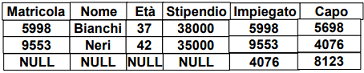
\includegraphics{images/61.PNG}
\end{center}
Ho due impiegati che soddisfano le condizioni e un capo che non ha impiegati che guadagnano più di 40.000 euro. Ho tuple che fanno JOIN e tuple che non hanno fatto JOIN. Quanto fatto permette di svolgere l'operazione di differenza, che vedremo più avanti
\subsection{Proiezione generalizzata}
\[\pi_{F_1,F_2,F_3}(E)\]
Dove $F_1,F_2,F_3$ sono espressioni aritmetiche su attributi di $E$ e costanti. Creo "un nuovo" attributo derivante da un'espressione algebrica dipendente da altri attributi e da costanti. Vediamo un esempio con la seguente tabella
\begin{center}
	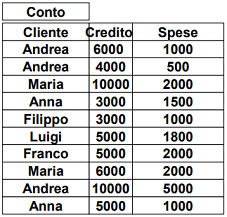
\includegraphics{images/62.PNG}
\end{center}
Posso scrivere, per esempio $\pi_{Cliente,Credito-Spese}(Conto)$, ottenendo
\begin{center}
	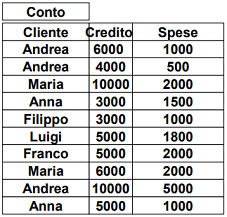
\includegraphics{images/62.PNG}
\end{center}
\subsection{Funzioni aggregate}
Si possono usare nelle espressioni dei nomi di funzione (operatori) che si applicano a insiemi e producono un valore scalare come risultato. Gli operatori aggregati sono:
\begin{itemize}
	\item \textbf{Somma}: $sum_{Spese}(Conto)$
	\item \textbf{Massimo}: $max_{Credito}(Conto)$
	\item \textbf{Minimo}: $min_{Credito}(Conto)$
	\item \textbf{Conteggio}: $count_{Cliente}(Conto)$
	\item \textbf{Conteggio di elementi distinti}: count-distinct$_{Cliente}(Conto)$
\end{itemize}
\subsection{Raggruppamento}
Posso raggruppare gli elementi di una relazione attraverso un apposito operatore. Posso raggruppare dei conti in base al codice cliente ravvicinando i conti correnti dei vari clienti. Posso applicare a questi gruppi degli operatori aggregati e ottenere un result set con una riga per ogni cliente.
\[_\mathbf{Cliente}G_{sum(Credito)}(Conto)\]
Posso avere più attributi con cui compiere il raggruppamento (a sinistra), ma anche più funzioni di aggregazione (a destra).
\subsection{Divisione}\footnote{Sezione da imparare come l'ave maria. La Vaglini chiede molto spesso di spiegare la divisione. Ringrazio Giovanni Ligato per avermi spiegato la cosa il giorno prima dell'orale (mi ha letteralmente salvato la vita).}
Operatore di tipo universale (parola chiave: tutti). Posso porlo sintatticamente all'interno di una query, ovviamente non è primitivo perchè corrisponde a un'espressione estremamente complessa.
\paragraph{Esempio} \emph{Trovare i nomi dei clienti che hanno un conto corrente in tutte le filiali di banca di Pisa}.\\Abbiamo le seguenti relazioni:
\begin{Verbatim}[commandchars=+\[\]]
	Branch(+underline[bank_name,branch_name], branch_city)
	Account(branch_name, bank_name, +underline[account_number], branch_city)
	Depositor(+underline[account_number], customer_name)
\end{Verbatim}
Possiamo risolvere l'esercizio attraverso la seguente espressione algebrica:
\[\Pi_{CN,BrN}(depositor \Join account) \div \Pi_{BrN}(\sigma_{BC='Pisa'}(branch))\]
Il risultato sono i clienti che hanno un conto in tutte le filiali di Pisa. L'espressione precedente, derivata, corrisponde alla seguente
\begin{align*}\Pi_{CN}(depositor \Join \sigma_{BC='Pisa'}(account)) - \Pi_{CN}(\\((\Pi_{CN}(depositor\Join \sigma_{BC='Pisa}(account)) \Join \Pi_{BrN}(\sigma_{BC='Pisa}(branch))\\-\\\Pi_{CN,BrN}(depositor \Join account)\\)\end{align*}
\begin{itemize}
	\item Prendo i clienti che esistono e hanno almeno un conto in una filiale di Pisa. 
	\item Attraverso un prodotto cartesiano (osservo dalle proiezioni che non metto insieme tuple con attributi comuni) genero tutte le coppie possibili tra i clienti che hanno conti a Pisa e le sedi di Pisa. Il risultato intermedio è caratterizzato da coppie veritiere (coloro che hanno effettivamente un conto in quella sede) e coppie false (persone che non hanno un conto in quella sede)
	\item Da questo prodotto cartesiano sottraggo le coppie veritiere (tutte, incluse quelle non di Pisa)
	\item La differenza più esterna mi porta ad ottenere coloro che hanno conti solo a Pisa.
	\item \textbf{Persona che ha conti solo a Pisa}: le coppie ottenute attraverso il prodotto cartesiano sono tutte veritiere. Segue che la differenza più interna le rimuoverà. Quindi la differenza più esterna non mi va a rimuovere questa persona.
	\item \textbf{Persona che non ha conti in tutte le filiali di Pisa}: le coppie ottenute attraverso il prodotto cartesiano sono in parte veritiere e in parte false. Attraverso la differenza più interna rimuovo le coppie veritiere. Mi rimangono le coppie false. Se ci sono coppie false significa che l'utente non ha conti in tutte le filiali di Pisa
\end{itemize}
%\paragraph{Quindi} La divisione consiste in una relazione su $R-S$. Date $r(R)$ e $s(S)$, con $R$ che contiene $S$, una tupla $t$ appartenente alla relazione divisione presenta le seguenti proprietà
%\begin{itemize}
%\item $t \in \Pi_{R-S}(r)$ (proiezione degli attributi della relazione $R-S$)
%\item $\forall t' \in s, \exists t'' \in r$ tale che
%\begin{itemize}
%\item $t'[S]=t''[S]$
%\item $t'[R-S]=t$
%\end{itemize}
%Per ogni tupla appartenente alla relazione $s$ esiste un'altra tupla appartenente alla relazione $r$ che sono uguali, con la proiezione degli attributi $S$. La seconda tupla, con gli attributi di $R-S$ è uguale a una tupla appartenente $\pi_{R-S}(r)$.
%\end{itemize}
\section{Relazioni derivate}
\paragraph{Relazioni di base} Presentano un contenuto autonomo
\paragraph{Relazioni derivate} Relazioni il cui contenuto è funzione del contenuto di altre relazioni. Quando compiamo un'interrogazione costruiamo dei risultati intermedi senza intaccare la base di dati. Potrei avere il bisogno di recuperare un risultato (anche più di una volta) assegnandogli un nome. Ciò consiste in una \emph{vista}. Essa può essere materializzata (salvata e usata più volte) o virtuale (usata una volta sola).
\begin{itemize}
	\item \textbf{Viste materializzate}: La memorizzazione risulta vantaggiosa perchè non hai da fare il calcolo tutte le volte (si hanno delle tabelle in carne ed ossa, ripensare a quanto visto con Pistolesi). I risultati sono immediatamente disponibili, ma potrebbero essere ridondanti e appesantire. Le viste materializzate non sono supportate da tutti i DBMS
	\item \textbf{Viste virtuali}: La vista virtuale è sempre ricalcolata ed è supportata da tutti i DBMS (nel db salviamo non il result set, ma lo snippet - il testo dell'interrogazione).
\end{itemize}
\paragraph{Colleghiamo a quanto fatto fino ad ora} Ottenere una vista significare dare un nome a un espressione. Esempio:
\[Supervisione = \pi_{Impiegato,Capo}(Afferenza \Join Direzione)\]
Posso adottare questa vista anche in altre espressioni:
\[\sigma_{Capo='Leoni'}(Supervisioni)\]
viene eseguita come
\[\sigma_{Capo='Leoni'}(\pi_{Impiegato,Capo}(Afferenza \Join Direzione))\]
\paragraph{Vantaggi per il programmatore} Possiamo semplificare la scrittura di interrogazioni seguendo il metodo del \emph{divide et impera} (divisione di un problema in sottoproblemi)
	\chapter{Mercoledì 25/03/2020}
\section{Ciclo di vita}
Il progetto è un'attività essenziale nella realizzazione di un software. Si parte da una serie di esgienze e si arriva a una base di dati che le soddisfa. Tutte le attività svolte per arrivare all'oggetto desiderato vanno a formare il \textbf{ciclo di vita}.
\begin{definizione}[Ciclo di vita]
	Sequenza di attività, anche ripetute ciclicamente, svolte da analisti, progettisti, utenti, nello sviluppo e nell'uso dei sistemi software.
\end{definizione}
\noindent Le fasi tipiche del ciclo di vita sono:
\begin{itemize}
	\item \textbf{Raccolta e analisi dei requisiti}: si cerca di capire cosa bisogna fare, quali proprietà dovrà avere il software da progettare;
	\item \textbf{Progettazione}: individuazione delle funzionalità richieste dal sistema e dei dati necessari;
	\item \textbf{Realizzazione} vera e propria;
	\item \textbf{Collaudo}: sperimentazione, verifica che quanto progettato sia corretto;
	\item \textbf{Operatività}: il sistema diventa operativo.
\end{itemize}
\section{Concentriamoci sulla progettazione}
La progettazione riguarda sia i dati che le funzionalità del sistema. Nel caso dei sistemi informativi (questi) la parte fondamentale è quella riguardante la progettazione dei dati.
\paragraph{Buon progetto} Un buon progetto presenta un'adeguata documentazione di quanto fatto. Si usano dei modelli per rappresentare i dati in modo formale, preciso e comprensibile: utilizzo quindi dei linguaggi che permettano di seguire tutta la fase di progettazione e verificare durante il progetto il modo in cui i requisiti sono rispettati.
\paragraph{Modello per il ciclo di vita} Esistono moltissimi modelli, il più vecchio e utilizzato è il \emph{Waterfall model}. Le fasi di vita sono attraversate in sequenza una dopo l'altra. ogni volta che si passa a una fase viene chiusa la precedente e questa non viene più ripetuta.\\
Qualunque sia il modello adottato si hanno delle sottofasi:
\begin{itemize}
	\item \textbf{Acquisizione dei requisiti}: dipende molto dai rapporti umani tra cliente e sviluppatore. Si tiene conto anche di normative, regolamenti e procedure aziendali, realizzazioni già esistenti
	\item \textbf{Analisi dei requisiti}: presenti una serie di linguaggi necessari per definire i requisiti da più punti di vista
\end{itemize}
\paragraph{Come si acquisiscono i requisiti?} I requisiti possono essere acquisiti mediante documentazione (normative, regolamenti e procedure aziendali, realizzazioni già esistenti) e direttamente dall'utente. Questo aspetto è il più complesso nel processo di acquisizione: gli utenti potrebbero fornire informazioni diverse (chi sta in alto potrebbe avere visione più ampia, ma meno dettagliata). Segue la necessità, nel corso della progettazione, di parlare più volte con chi di dovuto \emph{raffinando} le informazioni già in nostro possesso.
\paragraph{Ranking dei requisiti} Nella fase di progettazione è necessario tenere conto del \emph{ranking} dei requisiti: alcuni sono più importanti di altri.
\paragraph{Quando siamo in possesso della documentazione necessaria?} La regola fondamentale è leggere ogni singola cosa in nostro possesso: una singola parola può fare la differenza! Raggruppiamo le frasi generali e le frasi relative ai vari concetti. Per chiarire il termine di concetto solitamente si inserisce nel progetto un \emph{Glossario} (per ciascun elemento si indica una descrizione, eventuali sinonimi e collegamenti).
\subsection{Esempio concreto degli ultimi passi spiegati}
\textit{Si vuole realizzare una base di dati per una società che eroga corsi: di ogni corso vogliamo rappresentare i dati dei partecipanti e dei docenti. Per gli studenti (circa 5000), identificati da un codice, si vuole memorizzare il codice fiscale, il cognome, l'età, il sesso, il luogo di nascita, il nome dei loro attuali datori di lavoro, i posti dove hanno lavorato in precedenza insieme al periodo, l'indirizzo e il numero di telefono, i corsi che hanno già frequentato (le materie sono in tutto circa 200) e il giudizio finale.}
\subsubsection{Glossario dei termini}
\begin{center}
	\begin{tabular}{ |l|l|l|l| } 
		\hline
		\textbf{Termine} & \textbf{Descrizione} & \textbf{Sinonimi} & \textbf{Collegamenti}\\
		\hline
		Partecipante & Persona che partecipa ai corsi & Studente & Corso, Società\\
		\hline
		Docente & Docenti dei corsi, che può essere esterno. & Insegnate & Corso\\
		\hline
		Corso & Corso organizzato dalla società. Può avere più edizioni. & Materia & Docente\\
		\hline
		Società & Ente presso cui i partecipanti lavorano o hanno lavorato & Posti & Partecipante\\
		\hline
	\end{tabular}
\end{center}
\subsubsection{Frasi di carattere generale}
\textit{Si vuole realizzare una base di dati per una società che eroga corsi: di ogni corso vogliamo rappresentare i dati dei partecipanti e dei docenti.}
\subsubsection{Frase relative ai partecipanti}
\textit{Per i partecipanti (circa 5000), identificati da un codice, rappresentiamo il codice fiscale, il cognome, l'età, il sesso, la città di nascita, i nomi dei loro attuali datori di lavoro e di quelli precedenti (insieme alle date di inizio e fine rapporto), le edizioni dei corsi che stanno attualmente frequentando e quelli che hanno frequentato nel passato, con la relativa votazione finale in decimi.}
\subsubsection{Frasi relative ai datori di lavoro}
\textit{Relativamente ai datori di lavoro presenti e passati dei partecipanti, rappresentiamo il nome, l'indirizzo e il numero di telefono.}
\subsubsection{Frasi relative ai corsi}
\textit{Per i corsi (circa 200), rappresentiamo il titolo e il codice, le varie edizioni con date di inizio e fine e, per ogni edizione, rappresentiamo il numero di partecipanti e il giorno della settimana, le aule e le ore dove sono tenute le lezioni.}
\subsubsection{Frasi relative a tipi specifici di partecipanti - sottoclassi di partecipanti a cui si vuole dare una rappresentazione particolare}
\textit{Per i partecipanti che sono liberi professionisti, rappresentiamo l'area di interesse e, se lo possiedono, il titolo professionale. Per i partecipanti che sono dipendenti, rappresentiamo invece il loro livello e la posizione ricoperta.}
\subsubsection{Frasi relative ai docenti}
\textit{Per i docenti (circa 300), rappresentiamo il cognome, l'età, la città di nascita, tutti i numeri di telefono, il titolo del corso che insegnano, di quelli che hanno insegnato nel passato e di quelli che possono insegnare. I docenti possono essere dipendenti interni della società di formazione o collaboratori esterni.}
\subsubsection{Morale della favola}
Non si inizia la progettazione finchè non si è letto tutto in modo adeguato.
\subsection{Progettazione per livelli di astrazione}
Si hanno vari livelli di astrazione per la progettazione:
\begin{itemize}
	\item \textbf{Livello concettuale}, il più esterno: esprime come deve essere fatto il sistema per rispettare i requisiti. Permette di vedere, nel nostro caso, l'organizzazione della base di dati
	\item \textbf{Livello logico}: si dice qualcosa sull'organizzazione dei dati. Le relazioni utilizzate, come sono collegate tra di loro...
	\item \textbf{Livello fisico}: vediamo dei blocchi in memoria secondaria. Si decide l'allocazione dei dati e le modalità di accesso nei momenti di lettura.\footnote{Un esempio di cosa da fare potrebbe essere uno studio sulle relazioni per valutare la creazione di uno o più indici, in modo tale da velocizzare le operazioni più frequenti}
\end{itemize}
Questi livelli di astrazione corrispondono a degli schemi in cui si usano modelli e linguaggi differenti per descrivere ciò che si rappresenta in ogni livello.
\begin{center}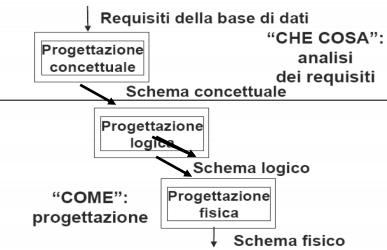
\includegraphics{images/3.PNG}\end{center}
\paragraph{Come si passa da un livello a un altro?} Facciamo una progettazione concettuale, li mettiamo nella rappresentazione, li verifichiamo e se tutto è valido compiamo un passaggio automatico da progettazione concettuale a progettazione logica. Se il progetto concettuale è ben fatto il progetto logico presenta esattamente le stesse proprietà. Il passaggio da progetto logico a fisico, invece, non è così automatico. Dopo la conclusione di una fase di progettazione si passa a quella successiva e non si ritorna più su quelle precedenti.
\subsection{Modelli concettuali}
Abbiamo bisogno di un buon linguaggio per descrivere lo schema concettuale. Abbiamo bisogno di un modello astratto il più vicino possibile all'essere umano: generalmente sono grafici semplici da usare e utili per interagire col cliente (quindi facilmente comprensibili anche da non-tecnici). I modelli esistenti sono formali (definiti in modo non ambiguo, descrivono in modo chiaro le caratteristiche di una base di dati) e integrati (descrivono tutte le caratteristiche della base di dati).
\begin{center}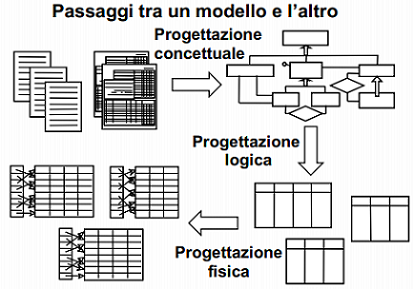
\includegraphics{images/4.PNG}\end{center}
\section{Modello E-R} Il modello più utilizzato è quello E-R (\emph{Entity-Relationship}): esso è il modello standard per descrivere una base di dati a livello concettuale.
\subsection{Costrutti del modello E-R}
Abbiamo tre costrutti di base: entità, relazioni e attributi. Si aggiungono i seguenti: identificatore e generalizzazione.
\subsubsection{Entita (\emph{entity})}
Un'entità è una classe di oggetti esistenti. Intendiamo fatti, persone, cose, impiegati, città, fatture, conti correnti... Ad ogni elemento sono associate delle proprietà comuni e con esistenza autonoma.\\

\noindent \textbf{Occorrenza di entità} Un'occorrenza è un elemento appartenente alla classe. A questo livello di progettazione so che un impiegato, per esempio, avrà certe proprietà: non mi interessa sapere i valori esatti ma so che possiede certe proprietà.\\
\textbf{Rappresentazione grafica} L'entità si rappresenta con un rettangolo avente un nome al suo interno.\begin{center}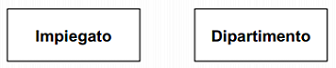
\includegraphics{images/5.PNG}\end{center}
\textbf{Convenzioni sui nomi} I nomi devono essere significativi (cioè che alludono in modo chiaro a cosa intendiamo) e possibilmente singolari.
\subsubsection{Associazioni (\emph{relationship})}
L'associazione è un legame fra due o più entità. Prendiamo per esempio studenti, esami e insegnamenti. Lo studente svolge un esame per un certo corso!	\\	

\noindent \textbf{Rappresentazione grafica} Le associazioni si rappresentano mediante rombi con all'interno il nome dell'associazione. Il rombo è collegato alle due entità collegate. Si osserva che non sono presenti frecce: non si ha un verso, chi viene prima e chi viene dopo non ha importanza.\begin{center}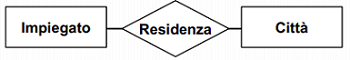
\includegraphics{images/6.PNG}\end{center}
\textbf{Convenzioni sui nomi} Anche qui i nomi devono essere espressivi e singolari. Importante usare sostantivi e non verbi: il verbo attribuisce un verso all'associazione e abbiamo detto che non ci sono frecce.\\
\textbf{Occorrenza di associazione} Un insieme di tuple, di occorrenze di entità. Se l'associazione è fra $t$ entità avrò $t$ tuple, ciascuna per ogni entità coinvolta. Non posso avere occorrenze ripetute, se ne ha una sola. L'occorrenza è definita come una coppia.
\paragraph{Domanda}
Questa base di dati consisterà in una rappresentazione del libretto elettronico o in un supporto a statini per la creazione di statistiche? Un uso diverso può comportare una progettazione diversa.
\begin{itemize}
	\item Se voglio realizzare semplicemente un libretto elettronico mi limito a indicare l'esame passato con la data e la valutazione
	\item Se voglio fare un supporto a statini allora ho bisogno di ulteriori informazioni: non soltanto l'ultimo esame passato ma anche i tentativi. Se progetto una base di dati come un libretto elettronico non posso trovare queste informazioni! Si deve organizzare la base di dati in modo che queste operazioni siano realizzabili: includeremo a tal proposito una nuova entità \emph{DataEsame}.
\end{itemize}
\paragraph{Passaggio da una rappresentazione per libretto a rappresentazione per supporto a statini}
\begin{center}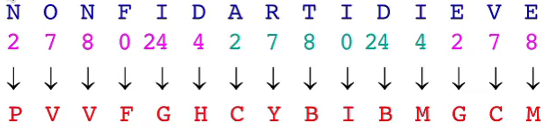
\includegraphics{images/9.PNG}\end{center}

\paragraph{Relationship diverse sulle stesse entità} Possono esistere più relazioni tra le stesse entità. L'impiegato può essere associato, per esempio, a due città: quella di residenza e quella di lavoro. Le due città possono coincidere ma possono essere anche diverse!
\begin{center}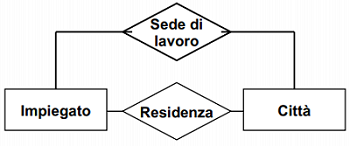
\includegraphics{images/10.PNG}\end{center}
\paragraph{Relationship ricorsiva} Un'entità può comparire più volte nell'associazione. Lego una persona, per esempio, a un'altra persona: ho l'occorrenza conoscenza che riguarda due persone che si conoscono. Posso stabilire, in alcuni casi, ruoli nella relazione ricorsiva: ho l'entità sovrano e la relazione successione, dove distinguo successore da predecessore.
\begin{center}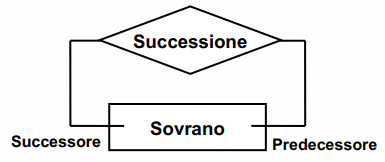
\includegraphics{images/11.PNG}\end{center}
\paragraph{Relationship mista} Posso mescolare ricorsione con ricorsione.

\subsubsection{Attributo}
Proprietà elementare di un'entità o di un'associazione.  L'attributo ha un certo dominio (o stringa, o intero, o data...) e il valore è associato ad occorrenze di entità o associazione.\\

\noindent \textbf{Rappresentazione grafica} Gli attributi si rappresentano attraverso grafi.
\begin{center}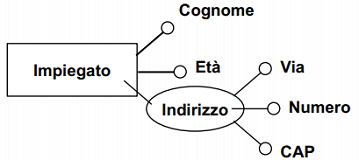
\includegraphics{images/12.PNG}\end{center}
Risulta possibile strutturare gli attributi in modo più dettagliato. Posso raggruppare parte degli attributi in un unico gruppo. La cosa è soprattutto grafica! Il nome dell'attributo composto è racchiuso all'interno di un "cerchio schiacciato".

\subsection{Esempio concreto}
\paragraph{Testo} \textit{Si vuole descrivere l'organizzazione di un'azienda
	\begin{itemize}
		\item Con sedi diverse
		\item Ogni sede è composta di vari dipartimenti
		\item Gli impiegati dell'azienda afferiscono ai vari dipartimenti e un'impiegato li dirige
		\item Gli impiegati lavorano su progetti
		\item Ogni entità o relationship può avere vari attributi
\end{itemize}}
\paragraph{Immagine} \begin{center}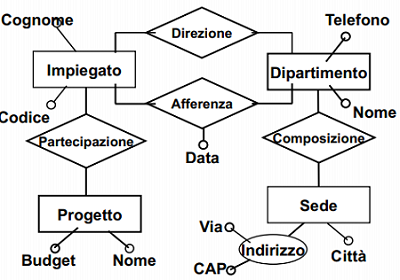
\includegraphics{images/17.PNG}\end{center}
\begin{itemize}
	\item Le entità presenti (concrete) sono Impiegato, Dipartimento, Progetto e Sede.
	\item Individuo gli attributi che descrivono le varie entità.
	\item Gli impiegati lavorano sui progetti, quindi stabilisco una relazione tra impiegato e progetto.
	\item L'impiegato afferisce a un dipartimento, cioè può decidere in quale dipartimento stare. Uno degli impiegati, inoltre, dirige un dipartimento
	\item In ogni sede ci sono più dipartimenti, ogni dipartimento ha una sede in cui è collocato.
\end{itemize}
\paragraph{Torno dal cliente e gli faccio vedere lo schema} Il cliente muove delle osservazioni, dettagli nuovi da aggiungere:
\begin{itemize}
	\item un dipartimento ha un solo direttore
	\item un impiegato può afferire ad un solo dipartimento
	\item il direttore di dipartimento afferisce a quel dipartimento
\end{itemize}
Lo schema è incompleto e non possiamo aggiungere i dettagli richiesti utilizzando solo i costrutti base.

\subsection{Cardinalità}
La cardinalità mi permette di stabilire, per esempio, quante coppie posso stabilire in un'associazione. Generalmente consiste in una coppia di valori associati a ogni entità che partecipa a una relazione: specifica il numero minimo e massimo di occorrenze della relazione cui ciascuna occorrenza di entità può partecipare.\\

\noindent \textbf{Rappresentazione grafica} La cardinalità si rappresenta etichettando le entità.\\
\textbf{Simbologia} I simboli adottabili nella cardinalità sono
\begin{itemize}
	\item numeri, ponibili sia nella cardinalità minima che in quella massima
	\item $N$, ponibile solo nella cardinalità massima, che attesta un numero formalmente illimitato di associazioni.
\end{itemize}
\textbf{Esempio grafico} \begin{center}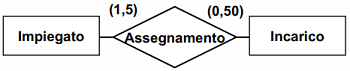
\includegraphics{images/14.PNG}\end{center}
\begin{itemize}
	\item Ogni impiegato ha un incarico ma non ne può avere più di cinque
	\item L'incarico può essere assegnato a un massimo di cinquanta persone, ma può essere anche non assegnato.
\end{itemize}
\textbf{Esempio grafico 2} \begin{center}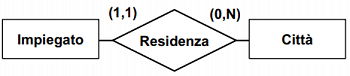
\includegraphics{images/15.PNG}\end{center}
\begin{itemize}
	\item L'impiegato è associato a una e una sola città di residenza
	\item La città può essere associata a un numero infinito di impiegati, ma può essere anche priva di relazioni con gli impiegati
\end{itemize}
\textbf{Tipi di relationship} Attraverso le cardinalità massime possiamo definire i seguenti tipi di relationship:
\begin{itemize}
	\item uno a uno (la cardinalità massima è sempre $1$)
	\begin{center}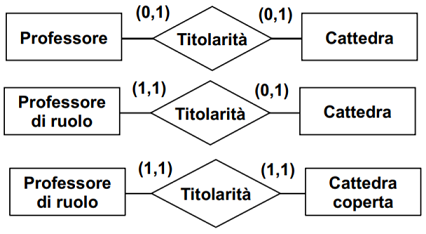
\includegraphics{images/149.PNG}\end{center}
	\item uno a molti (una delle due cardinalità massime è $1$, l'altra $N$)
	\begin{center}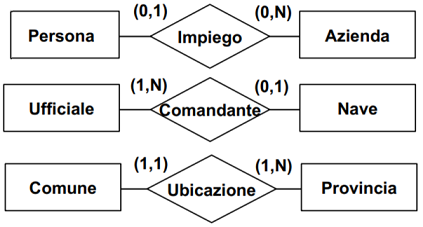
\includegraphics{images/147.PNG}\end{center}
	\item molti a molti (entrambe le cardinalità massime sono $N$)
	\begin{center}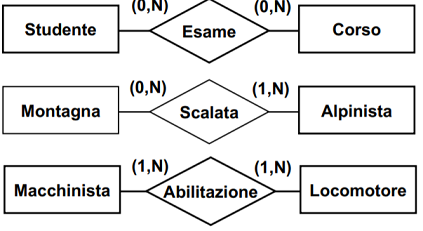
\includegraphics{images/148.PNG}\end{center}
\end{itemize}
\textbf{Cardinalità di attributi} Posso associare cardinalità anche agli attributi per indicare opzionalità dell'informazione o attributi multivalore.
\clearpage
\paragraph{Esempio cardinalità di attributi} \begin{center}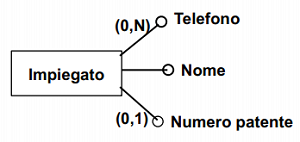
\includegraphics{images/16.PNG}\end{center}
\begin{itemize}
	\item L'impiegato può essere associato a un numero infinito di telefoni (non solo quello personale, ma anche quello aziendale...) o a nessun telefono
	\item L'impiegato può essere privo di patente o avere una sola patente.
\end{itemize}
\subsection{Riprendiamo lo schema E-R dell'azienda e poniamo le cardinalità}
\begin{center}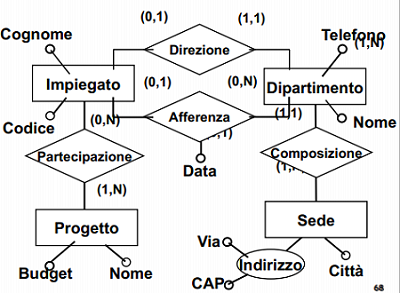
\includegraphics{images/18.PNG}\end{center}
\begin{itemize}
	\item Il dipartimento ha uno e un solo direttore (c'è sempre, quando aggiungo un nuovo dipartimento conosco già il direttore). L'impiegato può essere direttore ma può anche non esserlo
	\item Il dipartimento può essere privo di afferenze ma ne può avere un numero illimitato. L'impiegato può non avere afferenza, ma ne ha al massimo una (quindi l'impiegato può decidere di porsi in un certo dipartimento anche dopo l'assunzione). Segue che la data di afferenza può essere assente, e che ce ne sia al massimo una.
	\item Il dipartimento può avere infiniti numeri di telefono, ma almeno uno.
	\item L'impiegato può essere assegnato a un numero infinito di progetti, ma potrebbe anche essere privo di incarichi. Un progetto deve avere almeno un impiegato incaricato (ovviamente non si hanno limiti nel numero di persone assegnabili a un progetto).
	\item Il dipartimento sta in una sola sede. La sede ha almeno un dipartimento, ma può ospitare più di un dipartimento
\end{itemize}
\paragraph{Ritorno nuovamente dal cliente} I primi due dettagli sono sistemati, l'ultimo (quello di afferenza del direttore di dipartimento) no! Per il controllo di questa cosa, basato su valori, dobbiamo aggiungere la data di inizio direzione in modo da poter verificare che il direttore abbia assunto l'incarico dopo aver afferito a un certo dipartimento.

\subsection{Identificatore di un'entità}
Con le cardinalità si impongono vincoli generali sulle occorrenze delle associazioni. La scelta dell'identificatore permette di arricchire ulteriormente lo schema: ne può avere più di uno, ma ne deve avere per forza uno.\\L'identificatore può essere, per esempio, la targa di un automobile (se abbiamo un'entità Automobile) o tre attributi (Cognome, Nome e DataNascita) per l'entità Persona.\\

\noindent \textbf{Identificatori esterni}: ho una base di dati con gli studenti di tutta Italia. Uno studente di un certo ateneo è identificato da una matricola: tuttavia potrei avere uno studente, in un altro ateneo, avente la stessa matricola. Quindi devo utilizzare come identificatore non solo la matricola, ma anche il nome dell'università: questo identificatore lo devo prendere da un'altra tabella per evitare che vengano inseriti atenei inesistenti (Per esempio l'\emph{ateneo di Fornacette}). Segue l'uso di un vincolo di integrità referenziale.\\
L'identificatore esterno può essere utilizzato solo con cardinalità $(1,1)$: se avessi uno studente iscritto a più università in Italia quanto detto non funzionerebbe.
\begin{center}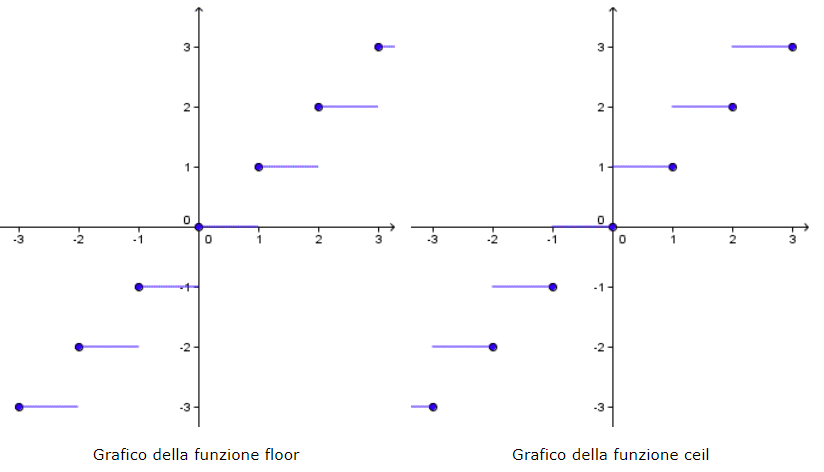
\includegraphics{images/19.PNG}\end{center}

\subsection{Mettiamo gli identificatori nello schema E-R}
\begin{center}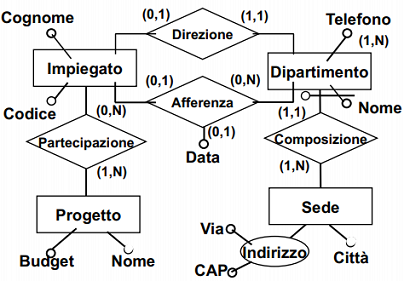
\includegraphics{images/20.PNG}\end{center}
\begin{itemize}
	\item Ogni impiegato ha un codice univoco identificativo
	\item Ogni progetto è identificato dal nome
	\item La sede è identificata dalla città (quindi una sola sede per città)
	\item Il dipartimento è identificato dal nome e dalla città (identificatore esterno)
\end{itemize}
Nelle associazioni non ho identificatori poichè l'identificatore è costituito dalla coppia associata.
\subsection{Generalizzazione}
La generalizzazione è un costrutto utile quando si stabilisce il modello concettuale ma che viene perso col passaggio ai modelli successivi. Si ha un concetto gerarchico. Ho l'entità Dipendente, posso stabilire l'esistenza di sue sottoclassi: impiegato, funzionario e dirigente. Sono distinti da attributi specifici che rendono diversa una sottoclasse dall'altra (lo stipendio, la residenza...).
\begin{center}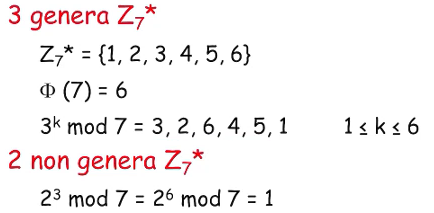
\includegraphics{images/23.PNG}\end{center}
Tutte le proprietà dell'entità genitore vengono ereditate dalle figlie e non rappresentate esplicitamente.\\
\textbf{Tipi di generalizzazione} La generalizzazione può essere
\begin{itemize}
	\item \textbf{Totale}: freccia piena, se ogni occorrenza dell'entità genitore è occorrenza di almeno una delle entità figlie (Esempio: le occorrenze di persona sono uomini o donne, nient'altro).
	\item \textbf{Parziale}: freccia vuota, esistono occorrenze dell'entità genitore che non sono occorrenze di entità figlie (Esempio: esistono occorrenze di persona che non sono nè studenti nè lavoratori).
\end{itemize}
La generalizzazione si dice:
\begin{itemize}
	\item \textbf{Esclusiva}: se ogni occorrenza dell'entità genitore è occorrenza di al più una delle entità figlie (Esempio: gli studenti lavoratori sono persone ma esistono occorrenze di persona che non sono ne studenti nè lavoratori).
	\item \textbf{Sovrapposta}: esistono occorrenze dell'entità genitore che sono occorrenze di più di una delle entità figlie (Esempio: ho uno studente lavoratore, un'occorrenza dell'entità persona è occorrenza sia di studente che di lavoratore).
\end{itemize}
\textbf{Gerarchia con una sottoclasse} Posso avere una gerarchia con una sola sottoclasse. Segue che avrò una generalizzazione di tipo parziale: è ovvio che se pongo solo una sottoclasse allora esisteranno occorrenze dell'entità genitore che non sono occorrenze dell'entità figlia (altrimenti farei prima a togliere il costruttore chiamando l'entità genitore come l'entità figlia).\\
\textbf{Alberi paralleli di gerarchia} Sono possibili alberi di gerarchia parallela, cioè fare partire più alberi dall'entità genitore. In questi alberi si distingue generalizzazione di tipo totale da generalizzazione di tipo parziale.
\begin{center}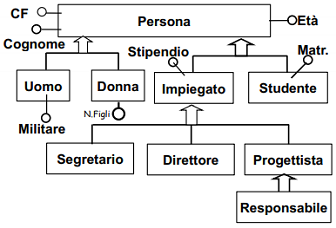
\includegraphics{images/22.PNG}\end{center}
\subsection{Documentazione associata agli schemi E-R}
\begin{center}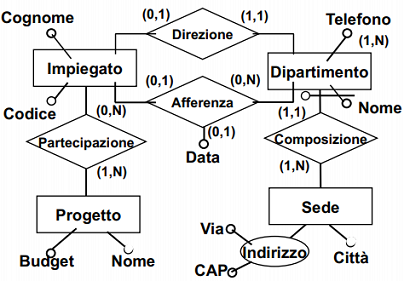
\includegraphics{images/20.PNG}\end{center}
Lo schema e basta non è mai sufficiente per rappresentare tutti i dettagli di un'applicazione. Ci sono vincoli non esprimibili (Esempio: il direttore che afferisce al dipartimento che dirige). Si pone in forma cartacea ciò che non è visibile dal grafico e anche ciò che lo è.
\subsubsection*{Dizionari dei dati (entità)} 
\begin{center}
	\begin{tabular}{ |l|l|l|l| } 
		\hline
		\textbf{Entità} & \textbf{Descrizione} & \textbf{Attributi} & \textbf{Identificatore}\\
		\hline
		Impiegato & Dipendente dell'azienda & Codice, Cognome & Codice\\
		\hline
		Progetto & Progetti aziendali & Nome, Budget & Nome\\
		\hline
		Dipartimento & Struttura aziendale & Nome, Telefono & Nome, Sede\\
		\hline
		Sede & Sede dell'azienda & Città, Indirizzo & Città\\
		\hline
	\end{tabular}
\end{center}
\subsubsection*{Dizionari dei dati (relationship)} 
\begin{center}
	\begin{tabular}{ |l|l|l|l| } 
		\hline
		\textbf{Relazioni} & \textbf{Descrizione} & \textbf{Componenti} & \textbf{Attributi}\\
		\hline
		Direzion & Direzione di un dipartimento & Impiegato, Dipartimento & \\
		\hline
		Afferenza & Afferenza a un dipartimento & Impiegato, Dipartimento & Data\\
		\hline
		Partecipazione & Partecipazione a un progetto & Impiegato, Progetto & \\
		\hline
		Composizione & Composizione dell'azienda & Dipartimento, Sede & \\
		\hline
	\end{tabular}
\end{center}
\subsubsection*{Regole di vincolo}
\begin{enumerate}
	\item Il direttore di un dipartimento deve afferire a tale dipartimento
	\item Un impiegato non deve avere uno stipendio maggiore del diretto del dipartimento al quale afferisce
	\item Un dipartimento con sede a Roma deve essere diretto da un impiegato con più di dieci anni di anzianità
	\item Un impiegato che non afferisce a nessun dipartimento non deve partecipare a nessun progetto
\end{enumerate}
\subsubsection*{Regole di derivazione}
\begin{enumerate}
	\item Il numero di impiegati di un dipartimento si ottiene contando gli impiegati che afferiscono a tale dipartimento
	\item Il budget di un progetto si ottiene moltiplicando per 3 la somma degli stipendi degli impiegati che vi partecipano
\end{enumerate}


\noindent I vincoli espressi in precedenza e le regole di derivazione riguardano i valori che vengono immessi nelle entità e associazioni in esecuzione.
\subsection{Quali costrutti scelgo?}
Per la scelta dei costrutti mi baso sulle loro definizioni
\begin{itemize}
	\item \textbf{Entità}: Se ha proprietà significativa e descrive oggetti con esistenza autonoma
	\item \textbf{Attributo}: Se è semplice e non ha proprietà
	\item \textbf{Associazione}: Se correla due o più concetti
	\item \textbf{Generalizzazione}: Se è caso particolare di un altro
\end{itemize}
\subsection{Quali caratteristiche deve avere il mio schema?}
Uno schema deve essere
\begin{multicols}{4}
	\begin{itemize}
		\item Corretto
		\item Completo 
		\item Leggibile
		\item Minimale 
	\end{itemize}
\end{multicols}
\subsection{Strategie di progetto}
\begin{itemize}
	\item \textbf{top-down}: parto da uno schema iniziale, lo raffino e integro mediante primitive che lo trasformano in una serie di schemi intermedi. Collego questi schemi e arrivo allo schema E-R finale. Le primitive di raffinamento sono:
	\begin{itemize}
		\item Da entità ad associazione tra entità
		\item Da entità a generalizzazione
		\item Da associazione a insiemi di associazioni
		\item Da associazione a entità con associazioni
		\item Introduzione di attributi su entità e associazioni
	\end{itemize}
	\item \textbf{bottom-up}: al contrario. Parto da specifiche iniziali, le divido fino a ottenere una specifica componente minima da cui nasce lo schema E-R. Gli schemi prodotti vengono fusi e integrati fino ad ottenere lo schema finale. Le primitive sono:
	\begin{itemize}
		\item Generazione di entità
		\item Generazione di associazione
		\item Generazione di generalizzazione
	\end{itemize}
\end{itemize}
Solitamente la strategia adottata è mista:
\begin{itemize}
	\item inizialmente individuo i concetti principali realizzando uno schema scheletro
	\item lo decompongo se necessario
	\item poi lo raffino, espando ed integro.
\end{itemize}
\paragraph{Definizione dello schema scheletro} Schema che contiene i concetti più importanti, i più citati o indicati esplicitamente come cruciali.

	\chapter{Mercoledì 01/04/2020}
\section{Esercitazione su progettazione}
\small
\subsection{Fasi del progetto}
Ricapitoliamo le varie fasi introdotte nella lezione precedente
\begin{itemize}
	\item \textbf{Analisi dettagliata delle specifiche fornite dal committente}\\ Questa fase è fondamentale per capire a fondo quali informazioni devono essere mantenute all’interno della base di dati. Scoprire in fase avanzata di progettazione che devono essere aggiunte nuove informazioni alla base di dati può essere molto costoso
	\item \textbf{Progettazione concettuale della base di dati}\\  Questa fase va dall’individuazione delle entità e delle relazioni, durante l’analisi delle specifiche, alla creazione dello schema concettuale (schema EntityRelationship)
	\item \textbf{Progettazione logica della base di dati}\\ Questa fase prende in pasto lo schema concettuale prodotto dalle fasi precedenti, e produce seguendo regole precise che richiedono poche scelte ulteriori lo schema logico (tabelle). 
	\item \textbf{Specifica dei vincoli}\\ Durante questa fase vengono specificati sia i vincoli di integrità referenziale (che derivano dalla traduzione in schema logico prodotta durante la fase precedente) che altri vincoli (necessari per mantenere la base di dati in uno stato consistente).
	\item \textbf{Realizzazione delle query}\\ Durante questa fase vengono create le query SQL che possono essere utilizzate per svolgere sulla base di dati le operazioni predefinite. 
\end{itemize}
\subsection{Specifiche di progetto}
\begin{itemize}
	\item Vogliamo progettare il sistema informativo di supporto ad un sito per l’acquisto di prodotti on-line. 
	\item Il sito potrà essere utilizzato solamente da utenti registrati, quindi anche gli acquisti possono essere effettuati solamente da utenti che si sono preventivamente registrati sul sito. Ovviamente è possibile che un utente sia registrato sul sito senza aver mai effettuato nessun acquisto. 
	\item I fornitori possono vendere i propri prodotti tramite il sito solo nel caso in cui siano preventivamente registrati. 
	\item I prodotti acquistati mediante il sito possono essere consegnati all’acquirente solamente da corrieri che siano preventivamente registrati sul sito.
	\item I fornitori offrono i propri prodotti, specificando prezzi e condizioni di vendita e di spedizione. 
	\item Uno stesso prodotto potrà essere venduto da fornitori diversi con prezzi e condizioni di vendita e spedizione diverse. 
	\item Il cliente sceglierà il fornitore da cui comprare un prodotto in base al suo criterio di scelta (a causa del prezzo, delle condizioni di vendita, ecc).
	\item Ciascun corriere metterà a disposizione della clientela vari tipi d consegna. 
	\item Ciascun fornitore registrato sul sito effettuerà accordi commerciali con alcuni dei corrieri registrati sul sito. 
	\item Nel momento in cui un fornitore decida di servirsi di un dato corriere, questi permetterà l’utilizzo di tutti i tipi di consegna messi a disposizione. 
	\item Nel momento in cui un cliente fa un ordine ad un fornitore potrà scegliere per la consegna solamente uno dei corrieri convenzionati con il fornitore. Ovviamente il cliente sceglierà il corriere in base a propri criteri (prezzo, tempi di consegna, garanzie offerte sulla consegna, ecc).
	\item Il sistema informativo dovrà mantenere anche informazioni sull’abbinamento di prodotti appartenenti a categorie diverse
	\begin{itemize}
		\item Ad esempio, se un cliente acquista un prodotto di categoria X, il sistema informativo dovrà essere in grado di consigliare i prodotti della categoria Y che sono abbinabili con il prodotto appena acquistato.
	\end{itemize}
	\item Nel caso in cui il cliente effettui un ordine tramite il sito potrà specificare il proprio grado di soddisfazione sull’operato del fornitore, inserendo nella base di dati un voto compreso tra 0 e 10. 
	\item Analogamente il cliente potrà specificare il proprio grado di soddisfazione sull’operato del corriere.
	\item Il voto che un cliente dà ad un fornitore o ad un corriere è legato ad un ordine e quindi ad una data.
	\item Sulla base di dati progettata dovranno essere effettuate delle query in grado di recuperare almeno le seguenti informazioni:
	\begin{itemize}
		\item Elenco di tutti i prodotti di una data categoria X che sono consigliati in seguito all’acquisto di un dato prodotto di categoria Y.
		\item Elenco dei fornitori che vendono il maggior numero di prodotti diversi di una data categoria X.
		\item Elenco dei fornitori che vendono un dato prodotto x a prezzo più basso.
		\item Elenco dei fornitori con voto medio più alto tra quelli che hanno un dato prodotto x presente in magazzino.
	\end{itemize}
	\item Inoltre sulla base di dati dovranno essere effettuate le seguenti operazioni:
	\begin{itemize}
		\item Inserimento di un nuovo ordine (con grado di soddisfazione del cliente nei confronti dell’operato del fornitore e del corriere nullo).
		\item Inserimento del grado di soddisfazione del cliente nei confronti dell’operato del fornitore e/o del corriere relativamente ad un ordine già effettuato.
		\item Inserimento di un nuovo prodotto nel magazzino di un fornitore (supponendo che tale prodotto fosse già presente all’interno della base di dati).
	\end{itemize}
\end{itemize}
\subsection{Individuazione entità}
\begin{itemize}
	\item Iniziamo la progettazione individuando le entità della base di dati:
	\begin{itemize}
		\item Gli Utenti sono registrati e costituiscono un’entità
		\item Un Prodotto è un’entità, la Categoria a cui appartiene può essere considerata come suo attributo
		\item La Spedizione (il tipo)
	\end{itemize}
	\item Possiamo specializzare Utente con Cliente, Fornitore e Corriere
	\item Otteniamo, quindi, la seguente situazione dove gli attributi in comune (Telefono, Indirizzo, e-mail, ecc) di Cliente, Fornitore e Corriere saranno attributi di
	Utente.
\end{itemize}
\begin{center}
	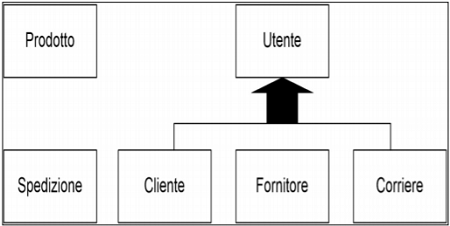
\includegraphics{images/86.PNG}
\end{center}
\begin{itemize}
	\item La base di dati deve tenere memoria degli ordini effettuati in modo che un voto possa essere assegnato sia ai fornitori che ai corrieri.
	\item Ciascun ordine consisterà delle seguenti informazioni:
	\begin{itemize}
		\item Cliente che ha effettuato l’ordine
		\item Fornitore che ha ricevuto l’ordine
		\item Corriere utilizzato per la consegna dell’ordine
		\item Tipo di spedizione utilizzato per recapitare l’ordine
		\item Prodotti acquistati tramite l’ordine
		\item Voto al corriere
		\item Voto al fornitore
	\end{itemize}
	\item Poiché un ordine non ha un’esistenza indipendente dalle altre entità (ad esempio un ordine non può esistere se non c’è un cliente che lo genera), possiamo classificare Ordine come una relazione.
	\item Ordine stabilisce un’associazione tra 5 entità diverse:
	\begin{itemize}
		\item Cliente
		\item Fornitore
		\item Corriere
		\item Spedizione
		\item Prodotti
	\end{itemize}
	\item Ed ha alcuni attributi propri: coto al corriere e voto al fornitore
	\item Nel ragionamento fin qui fatto abbiamo stabilito due punti che possono risultare difficili da gestire
	\begin{enumerate}
		\item una relazione connessa a 5 entità diverse pone problemi soprattutto per quanto riguarda l’individuazione delle cardinalità
		\begin{itemize}
			\item Possiamo pensare di raffinare (approccio topdown) la relazione Ordine in un’entità Ordine correlata alle 5 entità Cliente, Fornitore,.. da 5 relazioni diverse.
		\end{itemize}
		\item I prodotti hanno un attributo Categoria. Questa soluzione potrebbe dare origine a inconsistenze in fase di inserimento. Ad esempio, un fornitore potrebbe inserire
		\begin{itemize}
			\item Prodotto = “x”, Categoria = “RAM” 
			\item Prodotto = “y”, Categoria = “ram”
		\end{itemize}
		Come conseguenza nella base di dati i due prodotti risulterebbero appartenenti a categorie diverse
		\begin{itemize}
			\item Per evitare problemi di questo tipo possiamo effettuare ancora un raffinamento e trasformare Categoria in un’entità collegata a Prodotto da una relazione di appartenenza.
		\end{itemize}
	\end{enumerate}
	\item A questo punto lo schema delle entità risulterà il seguente: abbiamo una generalizzazione e alcune associazione già individuate
\end{itemize}
\begin{center}
	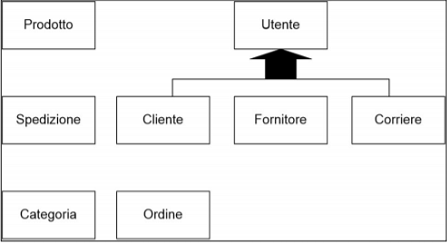
\includegraphics{images/87.PNG}
\end{center}
\subsection{Individuazione relazioni}
\begin{itemize}
	\item Occorre mettere in relazione l’entità Fornitore e l’entità Prodotto: introduciamo la relazione Vende
	\item Occorre mettere in relazione l’entità Fornitore e l’entità Corriere: introduciamo la relazione Accordo
	\item Occorre mettere in relazione l’entità Corriere e l’entità Spedizione: introduciamo la relazione Offre
	\item Occorre mettere in relazione l’entità Prodotto con se stessa per poter memorizzare l’abbinamento tra prodotti di categoria diversa: introduciamo la
	relazione Consiglia
\end{itemize}
\begin{center}
	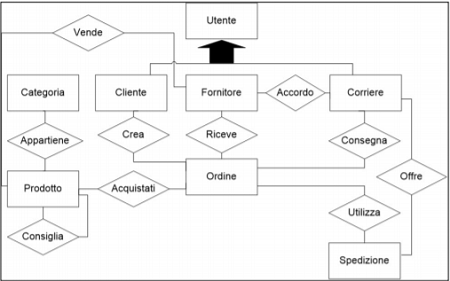
\includegraphics{images/88.PNG}
\end{center}
\subsection{Individuazione attributi}
\begin{itemize}
	\item Vediamo quali attributi associare alle varie entità: 
	\begin{itemize}
		\item Utente: Indirizzo, Telefono, E-mail,
		DataRegistrazione, UserName, Password
		\item Cliente: Nome, Cognome, CodFiscale
		\item Fornitore: RagSociale, PartitaIVA
		\item Corriere: RagioneSociale, PartitaIVA
		\item Categoria: CodCategoria, Descrizione \item Prodotto: CodProdotto, Marca, Modello, Descrizione, Foto
		\item Ordine: CodOrdine, DataEmissione, DataPagamento, TipoPagamento, DataConsegna, VotoFornitore, VotoCorriere
		\item Spedizione: AreaCoperta, DimMax, PesoMax
	\end{itemize}
	\item Non abbiamo associato il prezzo all’entità Prodotto perché un medesimo prodotto potrebbe essere venduto da fornitori diversi a prezzi diversi. 
	\item Analogamente non abbiamo associato il prezzo all’entità Spedizione perché supponiamo che uno stesso tipo si spedizione possa essere offerto da vari corrieri a prezzi diversi.
	\item Vediamo quali attributi potremmo associare alle varie relazioni:
	\begin{itemize}
		\item Vende: Prezzo, DispMagazzino
		\item Appartiene: nessun attributo
		\item Crea: nessun attributo
		\item Riceve: nessun attributo
		\item Acquistati: NumPezzi 
		\item Consiglia: nessun attributo
		\item Accordo: DataInizio, Durata
		\item Consegna: nessun attributo
		\item Utilizza: nessun attributo 
		\item Offre: Costo
	\end{itemize}
	\item Alla relazione Accordo abbiamo associato l’attributo DataInizio e Durata, ma supponiamo di non dover fare nessun controllo perché manterremo nella base di dati solamente gli accordi attualmente in vigore.
	\item Nella relazione Acquistati manteniamo memoria del numero di pezzi di ciascun prodotto richiesti in ciascun ordine
\end{itemize}
\begin{center}
	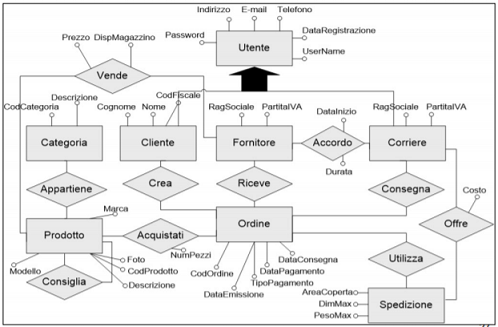
\includegraphics{images/89.PNG}
\end{center}
\subsection{Individuazione cardinalità}
\begin{itemize}
	\item Entità Ordine - Relazione Riceve: (1,1) in quanto un ordine viene ricevuto da un solo fornitore.
	\item Entità Ordine - Relazione Consegna: (1,1) in quanto un ordine viene recapitato da un solo corriere.
	\item Entità Ordine - Relazione Crea: (1,1) in quanto un ordine viene eseguito da un solo cliente.
	\item Entità Ordine - Relazione Utilizza: (1,1) in quanto per la consegna di un ordine si utilizza un solo tipo di spedizione.
	\item Entità Ordine - Relazione Acquistati: (1,N) in quanto un ordine può contenere più prodotti diversi.
	\item Entità Fornitore - Relazione Riceve: (0,N) in quanto un fornitore può aver ricevuto più ordini o nessun ordine (se ad esempio il fornitore si è appena iscritto al sito).
	\item Entità Fornitore - Relazione Accordo: (1,N) si suppone che, contemporaneamente all’iscrizione al sito, ogni fornitore si accordi con almeno un
	corriere.
	\item Entità Fornitore - Relazione Vende: (1,N) un fornitore può vendere più di un prodotto. Si suppone che, nel momento in cui si iscrive al sito, ogni fornitore sia in grado di vendere almeno un prodotto.
	\item Entità Corriere - Relazione Accordo: (0,N) un corriere può essere accordato con più fornitori o con nessun fornitore (ad esempio se si è appena iscritto al sito).
	\item Entità Corriere - Relazione Consegna: (0,N) un corriere può aver consegnato più ordini o nessun ordine (ad esempio se si è appena iscritto al sito).
	\item Entità Spedizione - Relazione Utilizza: (0,N) un tipo di spedizione può essere utilizzato per consegnare più ordini. È possibile però che un tipo di spedizione non sia mai stato utilizzato (ad esempio se è stato appena introdotto nel sito o se è particolarmente svantaggioso).
	\item Entità Spedizione - Relazione Offre: (1,N) un tipo di spedizione può essere offerto da più corrieri. Ciascun tipo di spedizione, però, deve essere offerto da almeno un corriere, altrimenti non avrebbe motivo di essere inserito nella base di dati del sito
	\item Entità Cliente - Relazione Ordine: (0,N) ciascun cliente può aver effettuato più ordini. È possibile che
	un cliente non abbia effettuato alcun ordine.
	\item Entità Prodotto - Relazione Vende: (1,N) un prodotto
	può essere venduto da più fornitori, e deve essere
	venduto da almeno un fornitore (altrimenti non
	avrebbe senso la presenza del prodotto nella base di
	dati del sito).
	\item Entità Corriere - Relazione Offre: (1,N) un corriere
	può offrire tipi di spedizione diversi. Si suppone che
	un corriere offra almeno un tipo di spedizione.
	\item Entità Prodotto - Relazione Consiglia: (1,N) ciascun
	prodotto ha almeno un altro prodotto consigliato.
	\item Entità Categoria - Relazione Appartiene: (1,N) la base
	di dati deve contenere almeno un prodotto per
	ciascuna categoria, infatti l’esistenza di una categoria
	vuota non avrebbe senso.
	\item Entità Prodotto - Relazione Appartiene: (1,1) ciascun
	prodotto appartiene ad una ed una sola categoria.
\end{itemize}
\begin{center}
	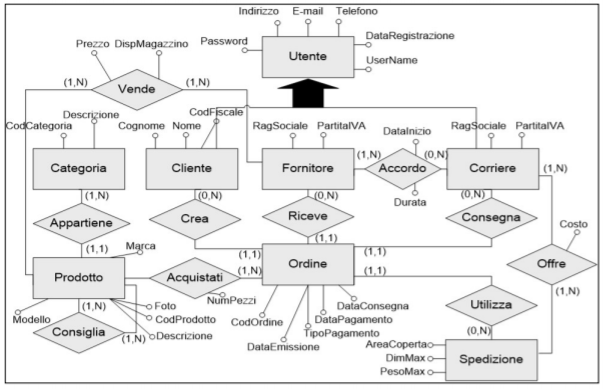
\includegraphics{images/90.PNG}
\end{center}
\subsection{Introduzione di nuovi attributi}
\begin{itemize}
	\item Se analizziamo le operazioni che devono essere compiute sulla base di dati ci rendiamo conto che potrebbe convenire introdurre dei nuovi attributi al fine di
	facilitarle. Questi attributi possono anche anche rappresentare informazione già presente nella base di dati.
	\item Consideriamo, ad esempio: elenco dei fornitori con voto medio più alto tra quelli che hanno un dato prodotto X presente in magazzino.
	\item In questo caso per recuperare il voto medio di un fornitore dobbiamo andare a leggere tutti gli ordini ricevuti da tale fornitore.
	\item Per facilitare questa operazione potremmo introdurre i seguenti attributi sull’entità Fornitore (perché non il voto medio direttamente?): TotaleVoti, NumeroVoti.
	\item In questo modo, ogni volta che introduciamo un ordine dovremo anche aggiornare questi attributi per il fornitore che ha ricevuto l’ordine.
	\item Quindi le operazioni coinvolte dall’introduzione di questi
	nuovi attributi sono le seguenti:
	\begin{itemize}
		\item Elenco dei fornitori con voto medio più alto tra quelli
		che hanno un dato prodotto x presente in magazzino.
		\item Inserimento del grado di soddisfazione del cliente
		nei confronti dell’operato del fornitore e/o del
		corriere in un ordine di cui si conosce il codice.
	\end{itemize}
	\item Per capire se l’introduzione dei nuovi attributi è
	vantaggiosa in termini di tempi di esecuzione, dobbiamo
	valutari i diversi costi per queste due operazioni.
\end{itemize}
\subsection{Riprendiamo le specifiche di progetto}
Al fine di prendere decisioni sulla struttura della base di dati, lo studente supponga che la base di dati
contenga:
\begin{itemize}
	\item 600 prodotti diversi
	\item 50 fornitori registrati
	\item 1500 clienti registrati
	\item 15 corrieri registrati
	\item 3 abbinamenti (in media) tra un prodotto x (di categoria X) e i prodotti della categoria Y.
	\item 5 ordini finora effettuati per ciascun prodotto.
\end{itemize}
\subsection{Tavola dei volumi}
\begin{itemize}
	\item Prima è necessario valutare il numero di istanze di una data entità o relazione. 
	\item Per fare questo dobbiamo basarci sulle indicazioni presenti all’interno delle specifiche. 
	\item Nel caso in cui queste non siano sufficienti, dovremo fare delle ulteriori ipotesi che faranno parte della descrizione finale della base di dati.\\
	\item Cliente: 1500 istanze (da specifiche) 
	\item Fornitore: 50 istanze (da specifiche) 
	\item Corriere: 15 istanze (da specifiche) 
	\item Utente: 1565 istanze (perché le persone che sono iscritte sia come clienti che come fornitori e/o corrieri
	hanno più di un account. Quindi gli utenti possono essere al più: 1565=1500+50+15) 
	\item Prodotto: 600 istanze (da specifiche) 
	\item Categoria: 30 istanze (supponiamo che la base di dati contenga 30 categorie diverse di prodotti) 
	\item Spedizione: 6 istanze (supponiamo che la base di dati contenga 6 tipi di spedizione diversi)
	\item Ordine: 3000 istanze (perché da specifiche vengono effettuati in media 5 ordini per ciascun prodotto: 3000=600*5) 
	\item Vende: 1800 istanze (supponiamo che ciascun fornitore venda in media 36 prodotti diversi: 1800=50*36) 
	\item Accordo: 150 istanze (supponiamo che ciascun fornitore si sia accordato in media con 3 corrieri diversi: 150=50*3) 
	\item Appartiene: 600 istanze (perchè ciascun prodotto appartiene ad una, ed una sola, categoria) 
	\item Crea: 3000 istanze (perché ciascun ordine è eseguito da un solo cliente) 
	\item Riceve: 3000 istanze (perché ciascun ordine è ricevuto da un solo fornitore)
	\item Consegna: 3000 istanze (perché ciascun ordine è recapitato da un solo corriere) 
	\item Utilizza: 3000 istanze (perché ciascun ordine è recapitato utilizzando un solo tipo di consegna) 
	\item Offre: 60 istanze (perché ciascun corriere offre in media 4 tipi di spedizione diversi: 60=15*4) 
	\item Acquistati: 6000 istanze (perché ciascun ordine comprende in media 2 prodotti diversi: 6000=3000*2) 
	\item Consiglia: 1800 istanze (perché da specifiche, ciascun prodotto ha in media 3 abbinamenti)
\end{itemize}
\subsection{Operazioni elementari}
\begin{itemize}
	\item Date le operazioni coinvolte
	\begin{itemize}
		\item Operazione 1: Elenco dei fornitori con voto medio più alto tra quelli che hanno un dato prodotto X presente in magazzino. 
		\item Operazione 2: Inserimento del grado di soddisfazione del cliente nei confronti dell’operato del fornitore e/o del corriere per un ordine di cui si conosce il codice. 
	\end{itemize}
	\item Dobbiamo individuare le operazioni elementari nei seguenti casi:
	\begin{itemize}
		\item svolgimento dell’operazione 1 senza nuovi attributi
		\item svolgimento dell’operazione 1 con nuovi attributi
		\item svolgimento dell’operazione 2 senza nuovi attributi
		\item svolgimento dell’operazione 2 con nuovi attributi
	\end{itemize}
	
	\item Esecuzione Operazione 1 senza attributi aggiuntivi:
	\begin{itemize}
		\item 1 lettura in Prodotto per recuperare il codice del prodotto
		\item 3 letture in Vende per recuperare il codice dei fornitori che vendono quel prodotto (un prodotto è venduto in media da 3 fornitori: 3=1800/600).
		\item 180 letture in Riceve per recuperare il codice degli ordini ricevuti dai fornitori che hanno quel prodotto
		in magazzino (ciascun fornitore riceve in media 60 ordini: 60=3000/50).
		\item 180 letture in Ordine per poter leggere il voto assegnato nei vari ordini ai fornitori che hanno quel prodotto in magazzino.
	\end{itemize}
	\item Esecuzione Operazione 1 con nuovi attributi:
	\begin{itemize}
		\item 1 lettura in Prodotto per recuperare il codice del
		prodotto
		\item 3 letture in Vende per recuperare il codice dei fornitori che vendono quel prodotto (un prodotto è venduto in media da 3 fornitori: 3=1800/600).
		\item 3 letture in Fornitore per recuperare il TotaleVoti e
		il NumeroVoti di ciascun fornitore che ha quel
		prodotto in magazzino.
	\end{itemize}
	\item Esecuzione Operazione 2 senza attributi aggiuntivi:
	\begin{itemize}
		\item 1 scrittura in Ordine per inserire un voto non nullo
	\end{itemize}
	\item Esecuzione Operazione 2 con attributi aggiuntivi:
	\begin{itemize}
		\item 1 scrittura in Ordine
		\item 1 lettura in Riceve per recuperare il fornitore che ha ricevuto l’ordine
		\item 1 lettura in Fornitore per recuperare il TotaleVoti e NumeroVoti
		\item 1 scrittura in Fornitore per scrivere il nuovo valore di TotaleVoti e NumeroVoti
	\end{itemize}
\end{itemize}
\subsubsection{Conclusioni}
\begin{itemize}
	\item Operazioni necessarie per svolgere l’operazione 1:\\363 letture $\to$ 363 operazioni elementari 
	\item Operazioni necessarie per svolgere l’operazione 1 con attributi aggiuntivi:\\ 6 letture $\to$ 6 operazioni elementari 
	\item Operazioni necessarie per svolgere l’operazione 2:\\ 1 scrittura $\to$ 2 operazioni elementari 
	\item Operazioni necessarie per svolgere l’operazione 2 con attributi aggiuntivi
	\begin{itemize}
		\item 2 scritture $\to$ 4 operazioni elementari
		\item 2 letture $\to$ 2 operazioni elementari
	\end{itemize}
	\item Supponendo che l’operazione 2 venga compiuta 10 volte più frequentemente rispetto all’operazione 1, avremo
	\begin{itemize}
		\item con i nuovi attributi:
		\begin{itemize}
			\item  6 Op. Elementari + 6*10 Op. Elementari 
			\item totale= 66 Op. Elementari
		\end{itemize}
		\item senza nuovi attributi:
		\begin{itemize}
			\item 363 Op. Elementari + 2*10 Op. Elementari 
			\item totale = 383 Op. Elementari
		\end{itemize}
	\end{itemize}
	\item Al fine di ridurre le operazioni elementari introduciamo i nuovi attributi all’interno dello schema ER.
\end{itemize}
\begin{center}
	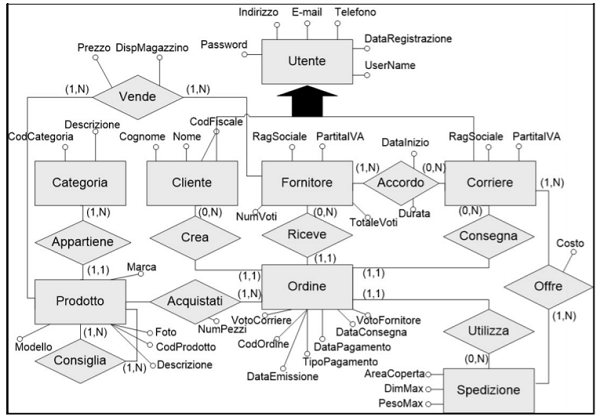
\includegraphics{images/98.PNG}
\end{center}
\subsection{Traduzione generalizzazioni}
\begin{itemize}
	\item Vediamo adesso come possiamo tradurre la generalizzazione presente nello schema ER. 
	\item Poiché si tratta di una generalizzazione totale, abbiamo tre possibilità:
	\begin{itemize}
		\item Lasciare padri e figli separati e collegarli utilizzando
		alcune relazioni.
		\item Accorpare l’entità padre sulle entità figlie
		\item Accorpare le entità figlie sull’entità padre. 
	\end{itemize}
	\item Analizziamo gli schemi ER che otteniamo in ciascuno di questi tre casi in modo da decidere quale di questi utilizzare.
\end{itemize}
\begin{center}
	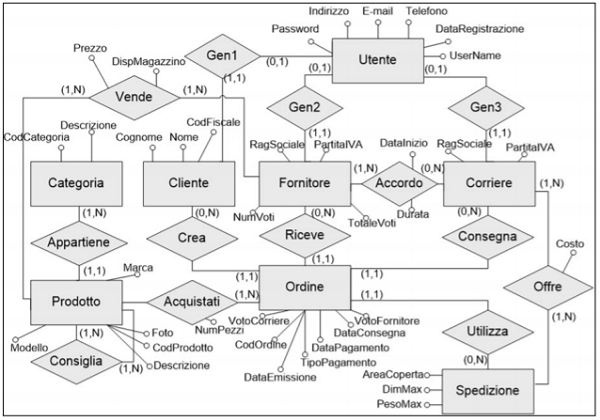
\includegraphics{images/97.PNG}
\end{center}
\begin{itemize}
	\item In questo modo abbiamo introdotto nello schema ER tre nuove relazioni. 
	\item Non abbiamo introdotto nessun valore NULL all’interno della base di dati.
	\item Abbiamo mantenuto un numero non troppo elevato di attributi per ciascuna entità
	\begin{itemize}\item quanto più il numero di attributi di un’entità è elevato, tanto più la gestione della relativa tabella diventa pesante. È quindi buona norma tentare di limitare il numero di attributi di ciascuna entità.\end{itemize}
\end{itemize}
\begin{center}
	\includegraphics{images/96.PNG}
\end{center}
\begin{itemize}
	\item In questo modo non abbiamo introdotto nello schema
	nessuna nuova relazione. 
	\item Non abbiamo introdotto nessun valore NULL all’interno
	della base di dati. 
	\item Abbiamo però aggiunto alle entità Cliente, Fornitore e Corriere molti nuovi attributi (evidenziati in rosso nello schema ER) ottenendo tabelle più pesanti da gestire. 
	\item Inoltre, quando vogliamo controllare la correttezza di una coppia (username, password) dovremo controllare le coppie (username, password) presenti in tre diverse tabelle (a meno che non si sappia in anticipo se tale coppia appartiene ad un cliente, ad un fornitore o ad un corriere). 
\end{itemize}
\begin{center}
	\includegraphics{images/95.PNG}
\end{center}
\begin{itemize}
	\item In questo modo non abbiamo introdotto nello schema ER
	nessuna nuova relazione. 
	\item Abbiamo però introdotto alcuni valori NULL all’interno dell’entità Utenti. 
	\item Il numero di attributi dell’entità Utenti è cresciuto
	molto. La tabella Utenti è molto pesante da gestire.
	\item Notare che anche se un fornitore vende
	necessariamente almeno un prodotto (cardinalità (1,N) tra la relazione Vende e l’entità Fornitori), non è detto
	che un utente (che può essere anche un cliente) venda necessariamente un prodotto (quindi cardinalità (0,N) tra la relazione Vende e l’entità Utenti). 
	\item Lo stesso vale per la relazione Accordo.\\
	
	\item Viste le tre possibili soluzioni, possiamo concludere che
	in questo caso conviene tradurre la generalizzazione
	lasciando l’entità padre e le entità figlie separate e
	collegate tramite relazioni. 
	\item In questo modo non introduciamo nessun valore NULL e
	il numero di attributi di ciascuna entità resta
	sufficientemente limitato. 
\end{itemize}
\begin{center}
	\includegraphics{images/94.PNG}
\end{center}
\subsection{Specifica chiavi}
Adesso dobbiamo specificare le chiavi delle varie entità:
\begin{itemize}
	\item Categoria: utilizziamo CodCategoria come chiave. 
	\item Prodotto: utilizziamo come chiave la coppia CodProdotto (attributo di prodotto) e CodCategoria
	(chiave dell’entità Categoria). 
	\item Ordine: utilizziamo CodOrdine come chiave. 
	\item Utente: utilizziamo UserName come chiave, in quanto ogni utente è caratterizzato dal proprio username. 
	\item Fornitore: potremmo utilizzare PartitaIVA come chiave, in quanto ogni fornitore è caratterizzato dalla propria partita IVA. In questo caso, peró, utilizzeremo come chiave lo UserName dell’utente associato.
	\item Corriere: potremmo utilizzare PartitaIVA come chiave, in quanto ogni corriere è caratterizzato dalla propria partita IVA. In questo caso, peró, utilizzeremo come chiave lo UserName dell’utente associato. 
	\item Cliente: potremmo utilizzare CodFiscale come chiave,
	in quanto ogni corriere è caratterizzato dal proprio codice fiscale. In questo caso, peró, utilizzeremo come chiave lo UserName dell’utente associato. 
	\item Spedizione: per identificare la spedizione dovremmo utilizzare gli attributi AreaCoperta, DimMax e PesoMax. Poiché utilizzare tre attributi come chiave
	può risultare scomodo, possiamo aggiungere un attributo CodSpedizione ed utilizzarlo come chiave.
\end{itemize}
\begin{center}
	\includegraphics{images/93.PNG}
\end{center}
\subsection{Traduzione in tabelle}
\begin{itemize}
	\item Traduciamo lo schema ER ottenuto in tabelle
	\item Ciascuna entità viene tradotta in una tabella a se stante
	\item Vediamo come tradurre le varie relazioni:
	\begin{itemize}
		\item Gen1: la traduciamo accorpando la tabella sull’entitá Cliente (cardinalitá (1,1) tra la relazione Gen1 e
		l’entitá Clente) 
		\item Gen2: la traduciamo accorpando la tabella sull’entitá Fornitore (cardinalitá (1,1) tra la relazione Gen2 e
		l’entitá Fornitore) 
		\item Gen3: la traduciamo accorpando la tabella sull’entitá Corriere (cardinalitá (1,1) tra la relazione Gen3 e
		l’entitá Corriere) 
		\item Vende: la traduciamo in una tabella a sé stante (relazione da N a N)
		\item Accordo: la traduciamo in una tabella a sé stante (cardinalitá (1,N) tra la relazione Accordo e l’entitá Fornitore e cardinalitá (0,N) tra la relazione Accordo e l’entitá Corriere) 
		\item Appartiene: la traduciamo accorpando la tabella sull’entitá Prodotto (cardinalitá (1,1) tra la relazione Appartiene e l’entitá Prodotto) 
		\item Crea: la traduciamo accorpando la tabella sull’entitá Ordine (cardinalitá (1,1) tra la relazione Crea e
		l’entitá Ordine) 
		\item Riceve: la traduciamo accorpando la tabella sull’entitá Ordine (cardinalitá (1,1) tra la relazione Riceve e
		l’entitá Ordine) 
		\item Consegna: la traduciamo accorpando la tabella sull’entitá Ordine (cardinalitá (1,1) tra la relazione Consegna e l’entitá Ordine)
		\item Utilizza: la traduciamo accorpando la tabella
		sull’entitá Ordine (cardinalitá (1,1) tra la relazione
		Utilizza e l’entitá Ordine) 
		\item Acquistati: la traduciamo in una tabella a sé stante
		(cardinalitá (1,N) tra la relazione Acquistati e l’entitá
		Ordine e cardinalitá (0,N) tra la relazione Acquistati
		e l’entitá Prodotto) 
		\item Offre: la traduciamo in una tabella a sé stante
		(relazione da N a N) 
		\item Consiglia: la traduciamo in una tabella a sé stante
		(relazione da N a N)
	\end{itemize}
	\item Quindi otteniamo le seguenti tabelle:
	\begin{figure}[h]
		\begin{subfigure}{0.5\textwidth}
			\includegraphics[width=0.9\linewidth]{images/91.PNG}
		\end{subfigure}
		\begin{subfigure}{0.5\textwidth}
			\includegraphics[width=0.9\linewidth]{images/92.PNG}
		\end{subfigure}
	\end{figure}
	
\end{itemize}
\subsection{Vincoli integritá referenziale}
Nel tradurre lo schema ER in tabelle, sono stati introdotti i seguenti vincoli di integritá referenziale:
\begin{itemize}
	\item  V.I.R.: tra l’attributo UserName della tabella Cliente
	e l’attributo UserName della tabella Utente.
	\item V.I.R.: tra l’attributo UserName della tabella
	Fornitore e l’attributo UserName della tabella
	Utente.
	\item V.I.R.: tra l’attributo UserName della tabella
	Corriere e l’attributo UserName della tabella Utente.
	\item V.I.R.: tra l’attributo CodCliente della tabella Ordine
	e l’attributo UserName della tabella Cliente.
	\item V.I.R.: tra l’attributo CodFornitore della tabella
	Ordine e l’attributo UserName della tabella
	Fornitore.
	\item V.I.R.: tra l’attributo CodCorrirere della tabella
	Ordine e l’attributo UserName della tabella Corriere
	\item V.I.R.: tra l’attributo CodSpedizione della tabella Ordine e l’attributo CodSpedizione della tabella Spedizione.
	\item V.I.R.: tra l’attributo CodCategoria della tabella Prodotto e l’attributo CodCategoria della tabella Categoria.
	\item V.I.R.: tra l’attributo CodCategoria della tabella Prodotto e l’attributo CodCategoria della tabella Categoria.
	\item V.I.R.: tra l’attributo CodFornitore della tabella
	Vende e l’attributo UserName della tabella Fornitore.
	\item V.I.R.: tra l’attributo CodProdotto della tabella Vende
	e l’attributo CodProdotto della tabella Prodotto.
	\item V.I.R.: tra l’attributo CodCategoria della tabella Vende e l’attributo CodCategoria della tabella Categoria.
	\item V.I.R.: tra l’attributo CodCategoria1 della tabella Consiglia e l’attributo CodCategoria della tabella Categoria.
	\item V.I.R.: tra l’attributo CodProdotto1 della
	tabella Consiglia e l’attributo CodProdotto della tabella Prodotto.
	\item V.I.R.: tra l’attributo CodCategoria2 della tabella Consiglia e l’attributo CodCategoria della tabella Categoria.
	\item V.I.R.: tra l’attributo CodProdotto2 della
	tabella Consiglia e l’attributo CodProdotto della tabella Prodotto.
	\item V.I.R.: tra l’attributo CodProdotto della
	tabella Acquistati e l’attributo CodProdotto della tabella Prodotto.
	\item V.I.R.: tra l’attributo CodCategoria della tabella Acquistati e l’attributo CodCategoria della tabella Categoria.
	\item V.I.R.: tra l’attributo CodOrdine della tabella
	Acquistati e l’attributo CodOrdine della tabella Ordine.
	\item V.I.R.: tra l’attributo CodCorriere della
	tabella Offre e l’attributo UserName della
	tabella Corriere.
	\item V.I.R.: tra l’attributo CodSpedizione della tabella Offre e l’attributo Cod Spedizione della tabella Spedizione.
\end{itemize}
\normalsize

\section{Implementazione dei vincoli}
L'algoritmo che ci permette l'uscita dallo schema E-R consiste in una serie di costrutti che permettono di creare le tabelle della nostra base di dati: le \emph{CREATE TABLE}.
\small
\begin{verbatim}
	CREATE TABLE Impiegato (
	Matricola CHAR(6) PRIMARY KEY,
	Nome CHAR(20) NOT NULL,
	Cognome CHAR(20) NOT NULL,
	Dipart CHAR(15),
	Stipendio NUMERIC(9) DEFAULT 0,
	FOREIGN KEY(Dipart) REFERENCES Dipartimento(NomeDip),
	UNIQUE(Cognome,Nome)
	)
\end{verbatim}
\normalsize
In questo caso abbiamo la relazione Impiegato, che presenta una serie di attributi. Ogni attributo è di un certo tipo e alcuni presentano delle clausole (\emph{keyword} associate agli attributi) per definire vincoli:
\begin{itemize}
	\item \textbf{Matricola} è la \emph{PRIMARY KEY}, ossia la chiave scelta per gli accessi dall'esterno. Segue che il valore dell'attributo non dovrà mai essere nullo e soprattutto essere unico, per permettere l'identificazione dei vari record. Il gestore verificherà che il valore indicato non sia già stato usato.
	\item \textbf{Nome} e \textbf{Cognome} sono \emph{NOT NULL}, cioè non possono essere mai vuoti.
	\item Con \emph{FOREIGN KEY} poniamo un vincolo di integrità referenziale. Si dice che l'attributo \textbf{Dipart} fa riferimento alla tabella Dipartimento, precisamente all'attributo \textbf{NomeDip}. Il valore indicato deve esistere come chiave nella tabella Dipartimento, altrimenti l'impiegato non viene inserito.
	\item Con \emph{UNIQUE} si stabilisce che non vi possono essere per forza aventi lo stesso \textbf{Nome} e \textbf{Cognome}.
\end{itemize}
\small
\begin{verbatim}
	CREATE TABLE Infrazioni(
	Codice CHAR(6) PRIMARY KEY,
	Data DATE NOT NULL,
	Vigile INTEGER NOT NULL REFERENCES Vigili(Matricola),
	Provincia CHAR(2),
	Numero CHAR(6),
	FOREIGN KEY(Provincia, Numero) 
	REFERENCES Auto(Provincia,Numero) ON DELETE SET NULL ON UPDATE CASCADE
	)	
\end{verbatim}
\normalsize
Qua abbiamo una tabella contenente le infrazioni. Ricordiamo quanto detto nella prima lezione: possiamo indicare il metodo per mantenere la consistenza della base di dati. Nell'esempio ho impostato la modifica del valore a NULL in caso di eliminazione e la modifica a cascata in caso di modifica.
\subsection{Vincoli di integrità generici: \emph{CHECK}}
Questi sono i vincoli basi garantiti al momento della tra duzione. Possiamo esprimere vincoli generici specificabili all'interno della tabella mediante la clausola \emph{CHECK}. Restringo i domini e specifico predicati (condizioni come quelle della clausola \emph{WHERE}) che devono essere soddisfatti ogni volta che un valore viene assegnato ad una variabile in quel dominio.
\begin{verbatim}
	CREATE TABLE Impiegato (
	Matricola CHARACTER(6),
	Cognome CHARACTER(20,
	Nome CHARACTER(20),
	Dipart CHARACTER(6),
	Ufficio CHARACTER(6),
	Sesso CHARACTER NOT NULL CHECK (Sesso IN('M','F')),
	Superiore CHARACTER(6),
	Stipendio INTEGER CHECK (Stipendio <= 
	(SELECT J.Stipendio FROM Impiegato AS J WHERE J.Matricola = Superiore)
	)
	)
\end{verbatim}
\begin{itemize}
	\item Voglio verificare che l'attributo \textbf{Sesso} assuma solo uno dei valori permessi (M, F)
	\item Voglio verificare che lo \textbf{Stipendio} dell'impiegato sia inferiore a quello del capo. Coinvolgo più attributi effettuando addirittura un'interrogazione.
\end{itemize}
La clausola CHECK può essere utilizzata all'interno della CREATE DOMAIN per stabilire un dominio.
\begin{verbatim}
	CREATE DOMAIN Voto 
	AS SMALLINT DEFAULT NULL
	CHECK (Value >= 18 AND Value <= 30)
\end{verbatim}
\subsubsection{ASSERTION}
Alcuni vincoli possono essere a livello non di un singola tabella ma di più tabelle. Attraverso un'asserzione, presente in una CREATE, stabilisco vincoli tra più tabelle.
\begin{verbatim}
	CREATE ASSERTION AlmenoUnImpiegato
	CHECK (1 <= (SELECT COUNT(*) FROM Impiegato))
\end{verbatim}
Con le asserzioni posso stabilire un qualunque vincolo predefinito: quando un'asserzione è stabilita ogni variazione del database è consentita solo se le asserzioni non vengono violate.
\subsubsection{Tipi di controllo} Si hanno due tipi di controllo
\begin{itemize}
	\item \textbf{Immediato}, verifica dopo ogni modifica
	\item \textbf{Differito}, verifica dopo una transazione (sequenza di operazioni)
\end{itemize}
Possiamo stabilire il tipo di controllo mediante il seguente costrutto
\begin{verbatim}
	SET CONSTRAINTS [NomeAss] (immediate | deferred)
\end{verbatim}
Un vincolo immediato non soddisfatto causa l'annullamento dell'operazione che ha causato la violazione (\emph{rollback parziale}), un vincolo differito non soddisfatto comporta l'annullamento di un'intera transazione (\emph{rollback}).
\paragraph{Nome delle asserzioni} Le asserzioni hanno un nome, quindi possono essere citate all'interno di istruzioni. Per esempio posso usare la seguente istruzione
\begin{verbatim}DROP NomeAss\end{verbatim} per eliminare l'asserzione con quel nome.
\subsection{Trigger}
Esiste un metodo diverso per inserire i vincoli, in un certo senso un vincolo dinamico. Esso reagisce in base a certi eventi avvenuti nel corso della computazione. Questi oggetti sono definiti \emph{trigger}.\\
Si stabiliscono delle condizioni che dovranno essere vere: se vere le istruzioni associate al trigger saranno eseguite. Abbiamo quindi i seguenti elementi:
\begin{itemize}
	\item \textbf{Evento} Solitamente si intendono modifiche dello stato del database: INSERT, DELETE, UPDATE. \\
	\small Se l'evento avviene il trigger è \emph{attivato} \normalsize
	\item \textbf{Condizione} La condizione che si deve verificare
	\small Se la condizione viene valutata il trigger è \emph{considerato} \normalsize
	\item \textbf{Azione} Ciò che viene eseguito con condizione vera
	\small Se l'azione è eseguita il trigger è \emph{eseguito} \normalsize
\end{itemize}
La sintassi dello standard attuale dell'SQL risale al 1999
\begin{verbatim}
	CREATE TRIGGER NomeTrigger
	{ BEFORE | AFTER } { INSERT | DELETE | UPDATE [of Column] } ON TabellaTarget
	[REFERENCING
	{[OLD TABLE [AS] VarTuplaOld] [NEW TABLE [AS] VarTuplaNew] } |
	{[OLD [ROW] [AS] VarTabellaOld] [NEW [ROW] [AS] VarTabellaNew] }
	]
	[FOR EACH { ROW | STATEMENT }]
	[WHEN Condizione]
\end{verbatim}
\subsubsection{Tipi di eventi}
\paragraph{BEFORE} Il trigger viene valutato prima della modifica dell'evento. Normalmente questa modalità è usata quando si vuole verificare una modifica prima che essa avvenga e "modificare la modifica"
\paragraph{AFTER} Prima si fa la modifica e successivamente si verificano le modifiche. Questa è la modalità più utilizzata.
\subsubsection{Granularità degli eventi}
\paragraph{Modalità di default \emph{statement-level}} Introdotta attraverso l'opzione \emph{for each statement}, il trigger viene considerato ed eseguito una volta sola per ogni statement che lo ha attivato, indipendentemente dal numero di tuple modificate.
\subsubsection{Conflitto tra trigger}
Se si hanno più trigger associati allo stesso evento possono emergere conflitti. Eseguo prima i BEFORE triggers e dopo la modifica gli AFTER triggers. Se i trigger appartengono alla stessa categoria l'ordine di esecuzione è stabilito in base alla data di creazione: i trigger più vecchi hanno priorità più alta.
\section{Istruzioni fondamentali per le transazioni}
\begin{itemize}
	\item BEGIN TRANSACTION: si specifica l'inizio di una transazione
	\item COMMIT WORK: la transazione è terminata con successo e quindi le operazioni specificate dopo la BEGIN TRANSACTION vengono eseguite sulla base di dati
	\item ROLLBACK WORK: si rinuncia all'esecuzione dell'operazioni specificate dopo la BEGIN TRANSACTION
\end{itemize}
\section{Integrazione con altri linguaggi di programmazione}
Abbiamo già visto che è possibile innesatare il linguaggio SQL con linguaggi di programmazione completamente diversi, per esempio il C++. Un precompilatore, legato al DBMS, viene usato per analizzare il programma e tradurlo in un programma nel linguaggio ospite (sostituendo le istruzioni SQL con chiamate alle funzioni di una API del DBMS). Tutto ciò avverrà ricorrendo a un'apposita libreria e dipenderà dal sistema operativo presente sulla macchina.
\paragraph{Attenzione} Il precompilatore è specifico per i linguaggi di programmazione coinvolti.
\paragraph{Conflitto di impedenza} Differenza tra ciò che può utilizzare un linguaggio di alto livello e ciò che SQL mette a disposizione. Il conflitto è risolto attraverso una tecnica detta \emph{cursore}: trasformiamo ciò che viene trasmesso dal DBMS, con il cursore scorriamo il buffer e leggiamo le tuple una alla volta. Successivamente il programma ricostituisce la struttura. Si ha una sorta di lettura da file dove il puntatore è appunto il cursore: si inizia un'operazione di lettura e alla fine si conclude con la chiusura del cursore.
\paragraph{SQL Statico ed SQL Dinamico} Le operazioni introdotte fino ad ora sono di tipo statico. Non sempre le istruzioni sono note quando scriviamo il programma! L'SQL dinamico permette la costruzione di istruzioni da parte del programma e non è banale gestire i risultati.\\
Un esempio si ha con la \emph{Call Level Interface}: si presuppone la presenza di un'interfaccia che chiede l'esecuzione di una certa operazione. Questo permette di interrogare un database anche con strutture diverse.
\paragraph{SQL Immerso VS CLI} La prima è più efficiente e permette l'esecuzione di tutte le funzioni di SQL. La CLI è indipendente, generica, permette di accedere a più basi, ma non fornisce tutte le funzionalità.
	\chapter{Giovedì 03/04/2020}

\section{Dal modello concettuale al modello logico}
\begin{wrapfigure}{r}{0.35\textwidth}
	\includegraphics[width=0.9\linewidth]{images/99.PNG} 
	\vspace*{-30pt}
\end{wrapfigure}

\paragraph{Obiettivo} Nel passaggio da modello concettuale a modello logico \emph{traduciamo} in modo automatico lo schema concettuale in uno schema logico che rappresenti gli stessi dati in maniera corretta ed efficiente. Nel compiere questo passaggio indichiamo come dati in ingresso:
\begin{itemize}
	\item lo schema concettuale
	\item il modello logico scelto
	\item le informazioni sul carico applicativo (dimensione dei dati)
\end{itemize}
Otteniamo, in uscita, lo schema logico.
\paragraph{No traduzione immediata} Prima di tradurre dobbiamo ristrutturare lo schema E-R. Obiettivo è:
\begin{itemize}
	\item semplificare (rimuovendo ciò che non può essere rappresentato nel modello logico) 
	\item ottimizzare (tenendo in conto i requisiti di prestazione).
\end{itemize}
\paragraph{Operazioni eseguibili nella ristrutturazione}
\begin{enumerate}
	\item Eliminazione delle generalizzazioni (come già detto vengono perse nel modello logico)
	\item Eliminazione degli attributi multivalore
	\item Analisi ed eventuale eliminazione/aggiunta di ridondanze
	\item Partizionamento/Accorpamento di entità e relationship
\end{enumerate}
\pagebreak
\small
\subsection{Eliminazione delle generalizzazioni}
Le gerarchie devono essere sostituite con entità e relazioni. Scegliamo la soluzione adatta in base al numero e al tipo degli accessi fatti alle singole entità per eseguire le operazioni. 
\begin{itemize}
	\item \textbf{Accorpamento delle figlie della generalizzazione nel genitore}. Questo tipo di sostituzione conviene quando gli accessi al padre e alle figlie sono contestuali.
	Le proprietà delle entità figlie vengono accorpate alle proprietà dell'entità genitore. Aggiungo un ulteriore attributo che mi permette di capire se un'occorrenza del genitore era occorrenza di uno dei figli (o di nessuno con generalizzazioni parziali)
	\begin{figure}[h]
		\begin{subfigure}{0.5\textwidth}
			\includegraphics{images/100.PNG} 
			\caption{Schema con generalizzazione}
		\end{subfigure}
		\begin{subfigure}{0.5\textwidth}
			\includegraphics{images/101.PNG}
			\caption{Schema ristrutturato}
		\end{subfigure}
	\end{figure}
	\item \textbf{Accorpamento del genitore della generalizzazione nelle figlie}. Questo tipo di sostituzione conviene con accessi solo alle figlie e questi sono distinti dall'una all'altra. Le entità figlie avranno anche gli attributi dell'entità genitore.
	\begin{figure}[h]
		\begin{subfigure}{0.5\textwidth}
			\includegraphics{images/102.PNG} 
			\caption{Schema con generalizzazione}
		\end{subfigure}
		\begin{subfigure}{0.5\textwidth}
			\includegraphics{images/103.PNG}
			\caption{Schema ristrutturato}
		\end{subfigure}
	\end{figure}
	\item \textbf{Sostituzione della generalizzazione con relazioni}. Questo tipo di sostituzione conviene  quando si effettuano accessi separati alle entità figlie e al padre. 
	Non effettuo trasferimenti di attributi, le due nuove entità sono identificate esternamente. In alcuni casi, in base al tipo di generalizzazione, potrei avere bisogno di stabilire dei vincoli di integrità.
	\begin{figure}[h]
		\begin{subfigure}{0.5\textwidth}
			\includegraphics{images/104.PNG} 
			\caption{Schema con generalizzazione}
		\end{subfigure}
		\begin{subfigure}{0.5\textwidth}
			\includegraphics{images/105.PNG}
			\caption{Schema ristrutturato}
		\end{subfigure}
	\end{figure}
\end{itemize}
\pagebreak
\paragraph{Soluzioni ibride} Individuiamo, soprattutto in gerarchie a più livelli, soluzioni ibride. 
\begin{figure}[h]
	\begin{subfigure}{0.5\textwidth}
		\includegraphics{images/105.PNG} 
		\caption{Schema con generalizzazione}
	\end{subfigure}
	\begin{subfigure}{0.5\textwidth}
		\includegraphics{images/106.PNG}
		\caption{Schema ristrutturato}
	\end{subfigure}
\end{figure}
\normalsize
\subsection{Eliminazione degli attributi multivalore}
\begin{wrapfigure}{r}{0.35\textwidth}
	\includegraphics{images/107.PNG} 
	\vspace*{-30pt}
\end{wrapfigure}
\paragraph{Pensiamo a delle soluzioni} Si potrebbe pensare a 
\begin{itemize}
	\item Ripetere le tuple con ogni valore diverso dell'attributo
	\item Una sola tupla dimensionata al numero massimo di numeri di telefono possibili
\end{itemize}
In entrambi i casi si ha spreco di memoria  e con la prima soluzione si potrebbe incorrere in inconsistenze. Segue che la migliore sostituzione consiste nello schema seguente
\begin{center}
	\includegraphics{images/108.PNG}
\end{center}
\subsection{Analisi ed eventuale eliminazione delle ridondanze}
\paragraph{Cos'è una ridondanza} Con ridondanza intendiamo un'informazione significativa, ma derivabile da altre.
\paragraph{Forme di ridondanza in uno schema E-R} 
\begin{itemize}
	\item attributi derivabili da altri attributi della stessa entità (o associazione)
	\begin{center}
		\includegraphics{images/109.PNG}
	\end{center}
	\item attributi derivabili da attributi di altre entità (o associazioni)
	\begin{center}
		\includegraphics{images/110.PNG}
	\end{center}
	\item associazioni derivabili dalla composizione di altre associazioni (presenza di cicli)
	\begin{center}
		\includegraphics{images/111.PNG}
	\end{center}
\end{itemize}
\subsubsection{Analisi di una ridondanza}
Abbiamo il seguente schema con ridondanza evidente (l'attributo \emph{Numero abitanti}).
\begin{center}
	\includegraphics{images/112.PNG}
\end{center}
Devo decidere se eliminare la ridondanza presente o mantenerla in base ad una valutazione del costo delle operazioni
\paragraph{\textcolor{green}{Vantaggi}} Interrogazioni semplificate
\paragraph{\textcolor{red}{Svantaggi}} Appesantimento degli aggiornamenti e maggiore occupazione di spazio
\paragraph{Come analizzo le prestazioni?} Per ottimizzare abbiamo bisogno di analizzare le prestazioni, ma come possiamo fare questo su uno schema concettuale? Prendiamo i seguenti indicatori di prestazione:
\begin{itemize}
	\item spazio: numero di occorrenze previste. Realizziamo una \textbf{tavola dei volumi} in cui elenchiamo i vari elementi e il loro volume (il numero di record).
	\item tempo: numero di occorrenze (di entità e relationship) visitate per portare a termine un'operazione. Partendo dai dati a disposizione costruisco una \textbf{tavola degli accessi} basata su uno schema di navigazione.
\end{itemize}
\subsubsection{Esempio di risoluzione (Mantenere il numeroAbitanti come attributo?)} Riprendiamo lo schema a inizio sessione. Vogliamo eseguire le seguenti operazioni:
\begin{itemize}
	\item \textbf{Operazione 1}: memorizza una nuova persona con la relativa residenza, supponendo che la città sia già presente (500 volte al giorno)
	\item \textbf{Operazione 2}: stampa tutti i dati di una città (incluso il numero di abitanti) (2 volte al giorno)
\end{itemize}
Devo decidere se mantenere l'attributo \emph{numeroAbitanti} o rimuoverlo. La tabella dei volumi è la seguente:
\begin{center}
	\includegraphics{images/113.PNG}
\end{center}
Analizziamo le tavole degli accessi con e senza ridondanza per entrambe le operazioni
\begin{figure}[h]
	\begin{subfigure}{0.5\textwidth}
		\includegraphics{images/114.PNG} 
		\caption{Accessi con ridondanza}
	\end{subfigure}
	\begin{subfigure}{0.5\textwidth}
		\includegraphics{images/115.PNG}
		\caption{Accessi senza ridondanza}
	\end{subfigure}
\end{figure}
\paragraph{Conclusioni} Se teniamo la ridondanza abbiamo:
\begin{itemize}
	\item Ho 1500 accessi in scrittura e 500 accessi in lettura al giorno per l'operazione 1
	\item L'operazione 2 è trascurabile.
\end{itemize}
Contando doppi gli accessi in scrittura (poichè hanno peso maggiore) otteniamo 3500 accessi al giorno. Consideriamo le stesse operazioni senza ridondanza, abbiamo:
\begin{itemize}
	\item Ho 1000 accessi in scrittura al giorno per l'operazione 1
	\item Ho 10.000 accessi in lettura al giorno per l'operazione 2
\end{itemize}
Contando doppi gli accessi (poichè hanno peso maggiore) in scrittura ho un totale di 12.000 accessi giornalieri.
\pagebreak
\subsection{Partizionamento/accorpamento di entità e relationship}
Le ristrutturazioni sono effettuate per rendere più efficienti le operazioni. Posso fare ciò \underline{riducendo gli accessi} con queste strategie
\begin{itemize}
	\item separare gli attributi di un concetto che vengono acceduti separatemente
	\item raggruppare attributi di concetti diversi acceduti insieme
\end{itemize}
Abbiamo i seguenti casi
\begin{itemize}
	\item Partizionamento di entità
	\begin{figure}[h]
		\begin{subfigure}{0.5\textwidth}
			\includegraphics{images/116.PNG} 
		\end{subfigure}
		\begin{subfigure}{0.5\textwidth}
			\includegraphics{images/117.PNG}
		\end{subfigure}
	\end{figure}
	\item Partizionamento di relationship
	\begin{figure}[h]
		\begin{subfigure}{0.5\textwidth}
			\includegraphics{images/120.PNG} 
		\end{subfigure}
		\begin{subfigure}{0.5\textwidth}
			\includegraphics{images/121.PNG}
		\end{subfigure}
	\end{figure}
	\item Accorpamento di entità/relationship
	\begin{figure}[h]
		\begin{subfigure}{0.5\textwidth}
			\includegraphics{images/118.PNG} 
		\end{subfigure}
		\begin{subfigure}{0.5\textwidth}
			\includegraphics{images/119.PNG}
		\end{subfigure}
	\end{figure}
\end{itemize}
\paragraph{Attenzione} Valutare osservando le cardinalità!
\subsection{Traduzione verso il modello relazionale} 
In questa traduzione:
\begin{itemize}
	\item Le entità diventano relazioni sugli stessi attributi
	\item Le associazioni diventano relazioni sugli identificatori delle entità coinvolte (più gli attributi propri)
\end{itemize}
\paragraph{Relationship molti a molti} Il seguente schema
\begin{center}
	\includegraphics{images/122.PNG}
\end{center}
Mi porta ad avere le seguenti relazioni
\begin{Verbatim}[commandchars=+\[\]]
	Impiegato(+underline[Matricola], Cognome, Stipendio)
	Progetto(+underline[Codice], Nome, Budget)
	Partecipazione(+underline[Matricola, Codice], DataInizio)
\end{Verbatim}
con i seguenti vincoli di integrità referenziale:
\begin{itemize}
	\item Matricola in Partecipazione e (la chiave di) Impiegato
	\item Codice in Partecipazione e (la chiave di) Progetto
\end{itemize}
\paragraph{Nomi più espressivi per gli attributi della chiave della relazione che rappresenta la relationship} I nomi degli attributi devono rendere chiara la relazione presente. Modifichiamo la relazione Partecipazione, che diventa così (ho alterato i nomi degli attributi chiave)
\begin{Verbatim}[commandchars=+\[\]]
	Partecipazione(+underline[Impiegato, Progetto], DataInizio)
\end{Verbatim}
\paragraph{Relationship ricorsive}
\begin{center}
	\includegraphics{images/123.PNG}
\end{center}
\paragraph{Relationship n-arie}
\begin{center}
	\includegraphics{images/124.PNG}
\end{center}
\pagebreak
\paragraph{Relationship uno-a-molti}
\begin{center}
	\includegraphics{images/125.PNG}
\end{center}
\paragraph{Non potrei ottenere una soluzione compatta?} Osservo che la cardinalità di Contratto rispetto a Giocatore è $(1,1)$. Posso rinunciare alla relazione Contratto ottenendo la seguente situazione
\begin{Verbatim}[commandchars=+\[\]]
	Giocatore(+underline[Cognome,DataNasc], Ruolo, Squadra, Ingaggio)
	Squadra(+underline[Nome], Città, ColoriSociali)
\end{Verbatim}
dove ho vincolo di integrità referenziale fra Squadra in giocatore e la chiave di squadra. Osservo che la cardinalità minima della relationship è 0 per Giocatore, segue che il valore dell'attributo Squadra, in Giocatore, può assumere valore nullo.
\paragraph{Entità con identificatore esterno}
\begin{center}
	\includegraphics{images/126.PNG}
\end{center}
\paragraph{Relationship uno-a-uno} Seguono due sempi dove variano le cardinalità

\begin{figure}[h]
	\begin{subfigure}{0.5\textwidth}
		\includegraphics[width=0.9\linewidth]{images/127.PNG} 
	\end{subfigure}
	\begin{subfigure}{0.5\textwidth}
		\includegraphics[width=0.9\linewidth]{images/128.PNG}
	\end{subfigure}
\end{figure}
	\chapter{Mercoledì 22/04/2020}
\section{Qualità delle relazioni}
Abbiamo progettato il nostro sistema attraverso un linguaggio concettuale, abbiamo utilizzato il modello E-R, abbiamo verificato le ridondanze e l'efficienza ottenendo alla fine il modello logico, cioè una serie di schemi di relazione. Adesso dobbiamo verificare la \emph{qualità delle relazioni}, cioè se presentano caratteristiche utili per il mantenimento della base di dati.
\paragraph{Obiettivo} Valutare la qualità della progettazione di schemi relazionali, capire se un raggruppamento di attributi in uno schema di relazione sia migliore di un altro.
\paragraph{Approccio adottato} \emph{top-down}.
\paragraph{Obiettivi impliciti}
\begin{itemize}
	\item Conservazione dell'informazione, cioè il mantenimento di tutti i concetti espressi mediante il modello concettuale, inclusi tipi di attributi, tipi di entità e tipi di associazioni.
	\item La minimizzazione delle ridondanze, cioè l'evitare la memorizzazione ripetuta della stessa informazione e quindi la necessità di effettuare molteplici aggiornamenti al fine di mantenere la consistenza tra le diverse copie della medesima informazione.
\end{itemize}
\paragraph{Linee guida}
\begin{itemize}
	\item \textbf{Semplice è bello}! Uno schema di relazione deve essere progettato in modo da rendere semplice la spiegazione del suo significato. Non devo raggruppare attributi provenienti da più tipi di entità e tipi di relazione in un'unica relazione. Se uno schema corrisponde a un solo tipo di entità o a un solo tipo di relazione risulta semplice spiegarne il significato, evitando così l'emergere di ambiguità semantiche.
	\item \textbf{Niente anomalie}! Gli schemi vanno progettati in modo da evitare anomalie nell'inserimento, nella cancellazione o nella modifica. Se possono presentarsi anomalie vanno rilevate e dobbiamo fare in modo che i programmi legati alla base di dati operino in modo corretto.
	\item \textbf{Evitare frequenti valori nulli}! Evitare di porre in una relazione attributi i cui valori possono essere frequentemente nulli. Se questi sono inevitabili ci si assicuri che si presentino solo in casi eccezionali rispetto al numero di tuple di una relazione. 
\end{itemize}
\paragraph{Esempio 1} Prendiamo la seguente relazione
\begin{verbatim}
	Fattura(CodF, CodProd, TotDaPagare, CostoNettoProd, IVA)
\end{verbatim}
Osservo che:
\begin{itemize}
	\item Il codice della fattura (CodF) determina il prodotto comprato, quindi il codice del prodotto (CodProd) e il costo totale (TotDaPagare)
	\item Il codice del prodotto (CodProd) determina il costo netto (CostoNettoProd) e l'iva da pagare (IVA)
	\item CostoNettoProd e IVA determinano quanto bisogna pagare (TotDaPagare)
\end{itemize}
Devo mantenere il tutto consistente. TotDaPagare è determinato da altri attributi, per evitare anomalie conviene rimuoverlo e calcolare il costo totale direttamente nella query.
\paragraph{Esempio 2} Prendiamo la seguente relazione
\begin{verbatim}
	Anagrafe(CF, NomeP, Indirizzo, NomeC, NumAb)
\end{verbatim}
Osservo che :
\begin{itemize}
	\item Il codice fiscale (CF) determina il nome della persona (NomeP), l'indirizzo (Indirizzo) e il nome della città (NomeC)
	\item Il nome della città (NomeC) determina il numero di abitanti (NumAb)
\end{itemize}
Il numero di abitanti è ripetuto tante volte quanti sono i residenti, questo valore deve essere mantenuto consistente (cioè uguale) per ogni persona di una certa città. Risulta ovvio che calcolare per ogni persona il numero di abitanti sia alquanto pesante. \textbf{Come risolviamo?} Trasformiamo Anagrafe in due schemi separati (con vincolo di integrità referenziale su NomeC e un vincolo aggiuntivo su NumAb)
\begin{verbatim}
	Persona(CF, NomeP, Indirizzo, NomeC)
	Residenza(NomeC, NumAb)
\end{verbatim}
\subsection{Approccio formale} 
Abbiamo visto che ci sono attributi che dipendono da altri attributi, devo verificare se ci sono troppe dipendenze tra gruppi di attributi all'interno di una tabella. A tal proposito parliamo di \textbf{dipendenze funzionali}, che esprimono legami semantici tra due gruppi di attributi di uno schema di relazione.
\begin{itemize}
	\item Una dipendenza funzionale è una proprietà dello schema di relazione, non di un particolare stato valido
	\item Una dipendenza funzionale non può essere dedotta a partire da uno stato valido, ma deve essere definita esplicitamente da qualcuno che conosce la semantica degli attributi (quindi non determino proprietà osservando i valori delle istanze, potrei confondere proprietà valide solo per quell'istanza con proprietà dello schema di relazione)
\end{itemize}
\paragraph{Definizione} Consideriamo la relazione $r$ su $R(X)$ e due sottoinsiemi non vuoti $Y$ e $Z$ di $X$. Si dice che esiste in $r$ una dipendenza funzionale da $Y$ a $Z$ se, per ogni coppia di ennuple $t_1$ e $t_2$ di r con gli stessi valori su $Y$ risulta che $t_1$ e $t_2$ hanno gli stessi valori anche su $Z$. \paragraph{Notazione} La notazione adottata è la seguente:
\[Y \longrightarrow Z\]
\paragraph{Attenzione} Non è detto che se io ho $Y \longrightarrow Z$ abbia il contrario, cioè $Z \longrightarrow Y$

\paragraph{Forma normale}
Attraverso le dipendenze funzionali esprimo tutto quello che so riguardante la base di dati. In base a queste dipendenze vorrei costruirmi una caratteristica dello schema per cui valgono quelle dipendenze: ciò significa che se quello schema presenta quelle caratteristiche allora si ha consistenza.\\
Questo schema è detto \textbf{forma normale}, che garantisce l'assenza di particolari difetti dallo schema (determina un livello di qualità). In base alle proprietà che ho dato posso determinare se lo schema si trova in una certa forma normale o in nessuna.
\paragraph{Normalizzazione} Se applico a un certo schema la definizione di forma normale e individuo che questo non è in tale forma, allora compio un processo di \emph{normalizzazione}. La normalizzazione è utilizzata come tecnica di verifica dei risultati della progettazione, non costituisce metodologia di progetto.
\paragraph{Esempio 3} Vediamo la seguente tabella contenente le informazioni di una certa azienda
\begin{center}
	\includegraphics{images/129.PNG}
\end{center}
Abbiamo i cognomi, gli stipendi, i progetti con il loro bilancio e la funzione nel progetto di ciascun dipendente. Ogni impiegato può partecipare a più progetti, sempre con lo stesso stipendio, e con una sola funzione per progetto. Neri, per esempio, lavora su tre progetti differenti.\\
Potrei incorrere nelle seguenti anomalie effettuando modifiche in modo scorretto:
\begin{itemize}
	\item \textbf{Anomalia di aggiornamento}: se lo stipendio di un impiegato varia è necessario andarne a modificare il valore più tuple
	\item \textbf{Anomalia di cancellazione}: se un impiegato si licenzia dobbiamo cancellarlo in diverse tuple (quindi rimuoverlo da tutti i progetti)
	\item \textbf{Anomalia di aggiornamento}: se un progetto varia il suo bilancio devo modificare l'attributo relativo in tutte le tuple dei dipendenti coinvolti nel progetto.
\end{itemize}
La causa sta, ovviamente, nella ripetizione dello stipendio di un impiegato e del bilancio di un progetto. L'errore è stato compiuto proprio nella fase di progettazione: abbiamo usato un'unica relazione per rappresentare gruppi di informazioni eterogenee. Trasformiamo le informazioni dette prima in dipendenze
\begin{itemize}
	\item Ogni impiegato ha un solo stipendio: Impiegato $\longrightarrow$ Stipendio
	\item Ogni progetto ha un solo bilancio: Progetto $\longrightarrow$ Bilancio
	\item Ogni impiegato ha una sola funzione per progetto: Impiegato Progetto $\longrightarrow$ Funzione
\end{itemize}
Osservando la tabella individuiamo pieno rispetto di queste dipendenze. \textbf{Ma ne esistono anche altre?} Abbiamo le cosiddette \textbf{dipendenze banali}, che sono sempre soddisfatte (proprietà ovvie di una relazione). Si osserva 
\[Impiegato\;Progetto \longrightarrow Progetto\]
Si dice che:
\begin{itemize}
	\item $Y \to A$ è non banale se $A$ non compare tra gli attributi di $Y$
	\item $Y \to Z$ è non banale se nessun attributo in $Z$ appartiene a $Y$.
\end{itemize}
\paragraph{Legame tra dipendenze e anomalie} Osserviamo che le prime due dipendenze comportano ripetizioni, mentre la terza no. Impiegato e Progetto non sono chiavi, Impiegato Progetto è chiave! La relazione contiene alcune informazioni legate alla chiave e altre ad attributi che non lo sono.

\subsection{Teoria delle dipendenze}
\subsubsection{Implicazione}
Sia $F$ un insieme di dipendenze funzionali definite su $R(Z)$ e sia $X \longrightarrow Y$.
\begin{itemize}
	\item Si dice che $F$ implica la dipendenza $X \to Y$ ($F \Rightarrow X \to Y$) se per ogni istanza $r$ di $R$ che verifica tutte le dipendenze in $F$, risulta verificata anche $X \to Y$.
	\item Si dice anche che $X \to Y$ è implicata da $F$
\end{itemize}
\subsubsection{Chiusura}
Dato un insieme di dipendenze funzionali $F$ definite su $R(Z)$ la chiusura di $F$ è l'insieme di tutte le dipendenze funzionali implicate da $F$.
\[F^{+}=\{X \to Y | F \Rightarrow X \to Y\}\]
Dato un insieme di dipendenze funzionali $F$ definite su $R(Z)$, un'istanza $r$ di $R$ che soddisfa $F$ soddisfa anche $F^{+}$.
\subsubsection{Superchiave}
Dato $R(Z)$ ed un insieme $F$ di dipendenze funzionali, un insieme di attributi $K$ appartenenti a $Z$ si dice superchiave di $R$ se la dipendenza funzionale $K \to Z$ è logicamente implicata da $F$ ($K\to Z$ è in $F^{+}$)
\paragraph{Chiave} Se nessun sottoinsieme proprio di $K$ è superchiave di $R$ allora $K$ si dice chiave di $R$.
\subsection{Calcolo di $F^{+}$ (regole di Armstrong)}
Utilizziamo un approccio costruttivo per arrivare all'algoritmo. Esistono una serie di regole, definite da \emph{Armstrong}, che mi permettono di arrivare a trovare l'insieme di tutte le dipendenze funzionali presenti nella chiusura.
\paragraph{Regole di inferenza di Armstrong}
\begin{itemize}
	\item \textbf{Riflessività}: se $Y \subseteq X$, allora $X \to Y$
	\item \textbf{Additività (o espansione)}: se $X \to Y$, allora $XZ \to YZ$ per qualunque $Z$
	\item \textbf{Transitività}: se $X \to Y$ e $Y \to Z$ allora $X \to Z$
\end{itemize}
\paragraph{Regole derivate di Armstrong}
\begin{itemize}
	\item \textbf{Regola di unione}: $\{X\to Y, X \to Z\} \Rightarrow X \to YZ$
	\item \textbf{Regole di pseudotransitività (o aggiunta sinistra)}: $\{X\to Y, WY \to Z\} \Rightarrow XW \to Z$
	\item \textbf{Regola di decomposizione}: se $Z \subseteq Y, X \to Y \Rightarrow X \to Z$
\end{itemize}
\paragraph{Proprietà delle regole di Armstrong}
\begin{itemize}
	\item \textbf{Teorema correttezza}: le regole di inferenze sono corrette, cioè, applicandole a un insieme F di dipendenze funzionali, si ottengono solo dipendenze logicamente implicate da F.
	\item \textbf{Teorema completezza}: le regole di inferenza sono complete, cioè, applicandole ad un insieme F di dipendenze funzionali, si ottengono tutte le dipendenze logicamente implicate da F.
	\item \textbf{Teorema minimalità}: le regole di inferenza sono minimali, cioè, ignorando anche una sola di esse, l'insieme di regole che rimangono non è più completo.
\end{itemize}
\paragraph{Esempio di dimostrazione} Dimostrare che per ogni istanza di relazione
\[X \to Y \Rightarrow XZ \to YZ\]
Supponiamo per assurdo che esista un'istanza $r$ di $R$ in cui valga $X \to Y$ ma non $XZ \to YZ$. Devono esistere due tuple $t_1$ e $t_2$ di $r$ tali che:
\begin{enumerate}
	\item $t_1[X]=t_2[X]$
	\item $t_1[Y] = t_2[Y]$
	\item $t_1[XZ]=t_2[XZ]$
	\item $t_1[YZ]\neq t_2[YZ]$
\end{enumerate}
Cioè è assurdo. Dalla prima e dalla terza deduciamo che
\[t_1[Z] = t_2[Z]\]
con questa e la seconda concludiamo che
\[t_1[YZ]=t_2[YZ]\]
in contraddizione con la quarta!

\paragraph{Riprendiamo l'esempio 3} Avevamo le seguenti dipendenze funzionali:
\begin{itemize}
	\item Impiegato $\longrightarrow$ Stipendio
	\item Progetto $\longrightarrow$ Bilancio
	\item Impiegato Progetto $\longrightarrow$ Funzione
\end{itemize}
Utilizzando la \emph{regola di attività} sulle prime due otteniamo
\begin{itemize}
	\item Impiegato Progetto $\longrightarrow$ Stipendio Progetto
	\item Impiegato Progetto $\longrightarrow$ Bilancio Impiegato
	\item Impiegato Progetto $\longrightarrow$ Funzione (Uguale a prima)
\end{itemize}
Infine, con la \emph{regola di unione}, avremo
\begin{itemize}
	\item Impiegato Progetto $\longrightarrow$ Stipendio Progetto Impiegato Bilancio Funzione
\end{itemize}
Quindi \underline{Impiegato Progetto} è chiave. Posso trovare altre dipendenze funzionali in $F^{+}$?
\subsection{Equivalenza}
Dato un insieme $F$ di dipendenze funzionali è molto utile poter determinare se un insieme $G$ sia equivalente ad $F$. Affermo che $F$ e $G$ sono equivalenti se
\[F^{+}=G^{+}\]
cioè per ogni $X \to Y \in F$ deve essere \[X \to Y \in G^{+}\] e, viceversa, per ogni $X \to Y \in G$ deve essere \[X \to Y \in F^{+}\]
\paragraph{Esempio} Supponiamo di avere questi due insiemi
\begin{align*}
	F&=\{\ A \to C, AC \to D, E \to AD, E \to H \}\\
	G&=\{\ A \to CD, E \to AH \}
\end{align*}
Voglio verificare l'equivalenza di $F$ e $G$. Devo dimostrare che le dipendenze funzionali in $F$ sono derivabili dalle dipendenze funzionali in G, e viceversa.
\begin{itemize}
	\item $A \to CD \Rightarrow \boxed{A \to C}, A \to D$
	\item $A \to CD, CCD \to CD \Rightarrow AC \to CD \Rightarrow AC \to C, \boxed{AC \to D}$
	\item $E \to AH \Rightarrow E \to A, \boxed{E \to H}$
	\item $E \to A, A \to D \Rightarrow E \to D$
	\item $E \to A , E \to D \Rightarrow \boxed{E \to AD}$
\end{itemize}
Ovviamente dovremo fare la stessa cosa al contrario. Da tutto questo capiamo quanto sia costoso il calcolo di $F^{+}$. Generalmente ci interessa sapere se $F^{+}$ contiene una certa dipendenza.
\paragraph{Chiusura transitiva} Come alternativa posso utilizzare la \emph{chiusura transitiva} di un insieme di attributi $X$ rispetto a $F$. Data una relazione $R(U)$, un insieme di attributi $X \subseteq U$, la chiusura detta consiste nell'insieme degli attributi che dipendono da $X$ (esplicitamente o implicitamente).
\[X^{+F}=\{A \;|\; A \in U\;\land\;F\Longrightarrow X \to A\}\]
Posso dimostrare che $X \to Y$ è in $F^{+}$ se $Y \subseteq X^{+}$
\paragraph{Riprendiamo l'esempio} Invece di verificare se $X \to Y$ in $F$ è anche in $G^{+}$ verifico se $Y \subseteq (X)^{+G}$ (chiusura di $X$ rispetto a $G$). Le varie chiusure qua sotto sono state trovate analizzando l'insieme di dipendenze funzionali $G$.
\begin{itemize}
	\item per $A \to C$ risulta $(A)^{+G}=ACD$. Ok ho $C \subseteq (A)^{+G}$
	\item per $AC \to D$ risulta $(AC)^{+G}=ACD$. Ok ho $D \subseteq (AC)^{+G}$
	\item per $E \to AD$ risulta $(E)^{+G}=EADCH$. Ok ho $AD \subseteq (E)^{+G}$
	\item per $E \to H$ risulta $(E)^{+G}=EHADC$. Ok ho $H \subseteq (E)^{+G}$
\end{itemize}
E viceversa per ogni dipendenza funzionale in G.

\paragraph{Esempio 2} Supponiamo di avere il seguente insieme
\[F = \{  A \to B, BC \to D, B \to E, E \to C \}\]
Calcoliamo $A^{+}$, cioè l'insieme di attributi dipendenti da $A$. Trovo che
\begin{itemize}
	\item $A^{+} = A$
	\item $A^{+} = AB$ poichè $A \to B$ e $A \subseteq A^{+}$
	\item $A^{+} = ABE$ poichè $B \to E$ e $B \subseteq A^{+}$
	\item $A^{+} = ABEC$ poichè $E \to C$ e $E \subseteq A^{+}$
	\item $A^{+} = ABECD$ poichè $BC \to D$ e $BC \subseteq A^{+}$
\end{itemize}
Quindi da $A$ dipendono tutti gli attributi dello schema, ovvero $A$ è superchiave oltre che chiave.
\subsection{Definizione aggiornata di equivalenza} Abbiamo modificato la definizione di equivalenza. Dati $F$ e $G$, essi sono equivalenti se
\begin{itemize}
	\item per ogni $X \to Y \in F, Y \in X^{+G}$, e
	\item per ogni $Z \to W \in G, W \in Z^{+F}$.
\end{itemize}
\subsection{Importanza della chiusura in un insieme di attributi} Dato $R(Z)$ con le sue dipendenze $F$, la chiusura di un insieme $X \subseteq Z$ di attributi è fondamentale per diversi scopi:
\begin{itemize}
	\item Possiamo verificare se una dipendenza funzionale è logicamente implicata da $F$
	\[X \to Y \in F^+ \Longleftrightarrow Y \subseteq X^{+F}\]
	\item Possiamo verificare se un insieme di attributi è chiave o superchiave:
	\begin{itemize}
		\item $X$ è superchiave di $R$ se e solo se $X \to Z \in F^+$, cioè se e solo se $Z \subseteq X^{+F}$
		\item $X$ è chiave di $R$ se e solo se $X \to Z \in F^+$ e non esiste alcun sottoinsieme $Y \subset X$ eliminando almeno un elemento, tale che $Z \subseteq Y^{+F}$
	\end{itemize}
\end{itemize}
\subsection{Ridondanze di un insieme di dipendenze funzionali}
Alcuni attributi di una dipendenza funzionale possono essere ridondanti. L'obiettivo è individuare forme equivalenti più semplici! Posso semplificare rimuovendo attributi sul lato sinistro di una DF (poichè non essenziali per determinare la parte destra) o rimuovere intere DF poichè ridondanti. Ricorriamo alle regole di Armstrong:
\begin{itemize}
	\item Applicazione della \emph{Regola di unione}: $\{A \to B, B \to C, A \to CD \}$ può essere semplificata in  $\{A \to B, B \to C, A \to C, A \to D \}$
	\item Attributi estranei a sx:  $\{A \to B, B \to C, AC \to D \}$ può essere semplificata in  $\{A \to B, B \to C, A \to D \}$
\end{itemize}
Un insieme $F$ di dipendenze funzionali può contenere dipendenze ridondanti, ovvero ottenibili tramite altre dipendenze di $F$. Ricorriamo alla transitività: $A \to C$ è ridondante in $\{A \to B, B \to C, \boxed{A \to C}\}$. Ricordiamo che la regola fondamentale è semplificare al massimo la rappresentazione dell'informazione.
\subsection{Dipendenze funzionali semplici}
Possiamo portare un insieme di dipendenze funzionali $F$ in forma standard, quella in cui sulla destra c'è un solo attributo.\\
Il seguente insieme 
\[F=\{AB \to CD, AC \to DE\}\]
Possiamo riscriverlo così
\[F=\{AB \to C, AB \to D, AC \to D, AC \to E\}\]
Quanto fatto è solo un primo step.
\subsection{Attributi estranei}
In alcune dipendenze funzionali è possibile che ci siano attributi inutili (appunto estranei) sul lato sinistro. Come li identifico?
\begin{itemize}
	\item Supponiamo di avere $F = \{AB \to C, A \to B\}$ 
	\item Ho $A^+=A$ e $B^+=B$
	\item $A^+=AB$ poichè $A \to B$ e $A \subseteq A^+$
	\item $A^+=ABC$ poichè $AB \to C$ e $AB \subseteq A^+$
\end{itemize}
$C$ dipende solo da $A$, e in $AB \to C$ l'attributo $B$ è estraneo poichè a sua volta dipende da $A$. Possiamo riscrivere l'insieme di dipendenze funzionali nel seguente modo
\[F^+ = \{ A \to C, A \to B\}\]
\paragraph{Morale della favola} In una dipendenza funzionale del tipo $AX \to B$ l'attributo $A$ è estraneo se $X^+$ include $B$ (ovvero $X$ da solo determina $B$).
\subsection{Algoritmo per la ridondanza di una dipendenza funzionale}
Dopo aver eliminato gli attributi estranei si deve verificare se sono presenti intere dipendenze funzionali inutili, cioè se intere dipendenze funzionali sono implicate da altre. Come faccio a capire se una dipendenza del tipo $X \to A$ è ridondante?
\begin{itemize}
	\item La elimino dall'insieme $F$
	\item Calcolo la chiusura di $X$ ($X^+$)
	\item Verifico se include $A$, cioè se con le dipendenze funzionali che restano riusciamo ancora a dimostrare che $X \to A$
\end{itemize}
\subsection{Copertura minimale}
Un insieme di dipendenze funzionali $F$ è minimale se:
\begin{itemize}
	\item Nella parte destra di ogni dipendenza funzionale c'è un solo attributo
	\item Non si possono togliere attributi nella parte sinistra di qualche FD senza perdere l'equivalenza nell'insieme ottenuto con $F$
	\item Non si possono togliere intere dipendenze funzionali senza perdere l'equivalenza nell'insieme ottenuto con $F$
\end{itemize}
Segue che una copertura minimale di un insieme $F$ è un insieme equivalente a $F$, ma di complessità minore.
\paragraph{NB} La copertura minimale non è unica.
\paragraph{Esempio di individuazione di copertura minimale} 
\begin{itemize}
	\item Abbiamo il seguente insieme: $F=\{ AB \to C, B \to A, C \to A \}$
	\item $A$ è estraneo in $AB \to C$, quindi: $F=\{ B \to C, B \to A, C \to A \}$
	\item $B\to A$ è ridondante, quindi ottengo: $F=\{ B \to C, C \to A \}$
\end{itemize}
Osserviamo che la dipendenze funzionale ridondante non può essere eliminata se prima non eliminiamo l'attributo estraneo. Segue l'importanza dello svolgere i passi spiegati nell'ordine mostrato!
	\chapter{Venerdì 24/04/2020}
\section{Forme normali e normalizzazione}
\subsection{Forma normale di Boyce-Codd (BCNF)}
Uno schema, se rispetta questa forma normale, è privo di informazione duplicata. Una relazione $r$ è in forma normale di Boyce-Codd se per ogni dipendenza funzionale (non banale) $X \to Y$ definita su di essa, $X$ è superchiave di $r$. Questa forma normale richiede che i concetti in una relazione siano omogenei (cioè che tutte le proprietà siano direttamente associate alla chiave)
\paragraph{Presenza di dipendenze non banali} Se un insieme $F$ di dipendenze per $R$ non è in BCNF, allora in $F$ c'è almeno una dipendenza $X \to Y$ non banale con $X$ non superchiave di $R$.
\paragraph{Teorema} Dato uno schema $R$ e un insieme $F$ di dipendenze funzionali, se $F$ non contiene alcune $X \to Y$ non banale con $X$ non superchiave di $R$, allora neanche $F^+$ la contiene.
\paragraph{Metodo di verifica} Analizzo una ad una le dipendenze non banali in $F$ verificando se ognuna ha una superchiave come membro sinistro.
\begin{itemize}
	\item Occorre saper verificare se $F$ è minimale
	\item Occorre saper verificare se un insieme di attributi è superchiave di una relazione.
\end{itemize}
\paragraph{Come normalizziamo?} Se una relazione non è in BCNF la rimpiazziamo con altre relazioni BCNF: faccio questo decomponendo sulla base delle dipendenze funzionali, \underline{separando i concetti}.
\begin{center}
	\includegraphics{images/142.PNG}
\end{center}
\paragraph{Esempio} Prendiamo la seguente tabella, che presenta certe dipendenze funzionali. 
\begin{center}
	\includegraphics{images/143.PNG}
\end{center}
Procediamo alla decomposizione, ottenendo quanto segue
\begin{center}
	\includegraphics{images/144.PNG}
\end{center}
Un buon indicatore della correttezza di quanto stiamo facendo è la ricomposizione della tabella iniziale dopo aver effettuato le divisioni: se non posso riottenere la relazione iniziale allora qualcosa non va. Si individua che alcune composizioni di Boyce-Codd potrebbero presentare questo problema
\begin{center}
	\includegraphics{images/145.PNG}
\end{center}
se io faccio JOIN con la sede ottengo tuple che precedentemente non esistevamo. Segue che dobbiamo trovare composizioni BCNF particolari!
\paragraph{Decomposizione senza perdita} Una istanza $r$ di una relazione $R$ si decompone senza perdita su $X_1$ e $X_2$ se il join naturale delle proiezione di $r$ su $X_1$ e $X_2$ è uguale ad $r$ stessa.
\paragraph{Algoritmo per la decomposizione in BCNF}  Assumiamo che tutte le dipendenze funzionali in $F$ abbiano un unico attributo come membro destro, e che $U$ sia l'insieme di tutti gli attributi di $R$.
\begin{itemize}
	\item $Decomponi(R,F)$
	\begin{itemize}
		\item Se esiste $X \to A$ in $F$ con $X$ non superchiave di $R$:
		\begin{itemize}
			\item Sostituisco $R$ con una relazione $R_1$ con attributi $U-A$ ed una relazione $R_2$ con attributi $X \cup A$
		\end{itemize}
		\item $Decomponi(R_1,F_{U-A})$
		\item $Decomponi(R_2,F_{X \cup A})$
	\end{itemize}
\end{itemize}
\paragraph{Esempio} Riprendiamo la solita tabella di prima. Abbiamo
\[F=\{Impiegato \to Sede, Progetto \to Sede \}\]
Applico l'algoritmo e ottengo
\[Decomponi(R,F)= R_1(Impiegato,Progetto), R_2(Impiegato, Sede)\]
\paragraph{Teorema, correttezza dell'algoritmo della decomposizione} Qualunque sia l'input, l'esecuzione dell'algoritmo su tale input termina e produce una decomposizione della relazione originaria tale che:
\begin{itemize}
	\item Ogni relazione ottenuta è in BCNF
	\item La decomposizione è senza perdita nel JOIN
\end{itemize}
\paragraph{Proiezione delle dipendenze funzionali di $R(U)$ su $X \subseteq U$} La proiezione di $F$ su $X$, denotata da $F_x$ è l'insieme delle dipendenze funzionali $Z \to Y$ in $F^+$ che coinvolgono solo attributi in $X$, cioè tali che $Z \subseteq X$ e $Y \subseteq X$.
\paragraph{Calcolare la proiezione delle DF su X}
\begin{itemize}
	\item CalcolaProiezione(F, X) :=
	\begin{itemize}
		\item Pongo $result = \{ \emptyset \}$
		\item Per ogni sottoinsieme proprio $S \subset X$, per ogni attributo $A \in X$ tale che $A \notin S$ e tale che non esiste alcun sottoinsieme $S'$ di $S$ tale che 
		\[S'\to A\]
		è in result, allora dico che se $A \subseteq S^{+}$ allora
		\[result=result \cup \{ S \to A \}\]
	\end{itemize}
\end{itemize}
Il metodo è funzionante ma in alcuni casi la proiezione di $F$ su $X$ può avere dimensione esponenziale rispetto alla dimensione di $F$ ed $X$. Si può dimostrare che nessun insieme equivalente a quello delle proiezioni non puiò avere cardinalità minore.
\paragraph{Esempio da internet per capire una spiegazione arzigogolata} Supponiamo di avere $R(A,B,C)$ e il seguente gruppo di dipendenze funzionali
\[F=\{ A\to B, B \to C, C \to A\}\]
individuo le seguenti proiezioni
\begin{itemize}
	\item $F_{AB}=\{ A \to B, B \to A\}$. 
	\item $F_{AC}=\{ A \to C, C \to A\}$
\end{itemize}
La prima proiezione è interessante perchè ci fa capire che non possiamo limitarci a verificare solo che $X \subseteq AB$ ed $Y \subseteq AB$ con $X \to Y$. Per comodità dobbiamo trovare, dato un insieme $F$, la sua copertura minimale. A quel punto dobbiamo stare attenti agli attributi sinistri, cioè controllare se essi non dipendono a loro volta dagli elementi su cui stiamo facendo la proiezione. In questo caso:
\begin{itemize}
	\item Pongo da $B \to C$ e $C \to A$
	\[BC \to A\]
	Ovviamente $C$ dipende da $B$ e per questo può essere rimosso.
	\item $BC$ è l'insieme $S$ che dicevamo nella spiegazione dell'algoritmo. In questo caso esiste un sottoinsieme $S'$ formato solo da $C$... Infatti possiamo dire che
	\[C \to A\]
\end{itemize}
\paragraph{Proprietà dell'algoritmo di decomposizione} A seconda dell'ordine con cui si considerano le dipendenze funzionali il risultato della decomposizione può cambiare. Riprendiamo l'esempio di prima e consideriamo le dipendenze funzionali in ordine diverso. Otteniamo uno schema diverso
\begin{verbatim}
	Rx(Impiegato, Sede)
	Ry(Impiegato, Progetto)
\end{verbatim}Supponiamo di voler inserire un nuovo impiegato, che sta a Milano, che lavorerà sul progetto Marte, con sede a Roma. 
\begin{center}
	\includegraphics{images/150.PNG}
\end{center}L'inserimento è legittimo ma emerge un'inconsistenza relativa alla sede della persona e la sede del progetto
\begin{center}
	\includegraphics{images/146.PNG}
\end{center}
Non capiamo più se la sede indicata è quella dell'utente o del progetto! Non ho perdita di informazione attraverso il JOIN (le tuple che già esistevano prima della divisione della relazione esistono), ma la tupla nuova rappresenta qualcosa di inconsistente (la sede di Marte è a Milano, quando in realtà il progetto ha sede a Roma).  Segue che quanto detto ci garantisce il JOIN ma non le dipendenze (nell'esempio sono state perse).
\paragraph{Verifica di decomposizione senza perdita di dipendenze} La definizione di decomposizione senza perdita di dipendenze (considerando due relazioni $R1(X)$ ed $R2(Y)$ ottenute dalla decomposizione) è basata sul verificare che
\[(F_X \cup F_Y)^+=F^+\]
cioè la chiusura dell'insieme $F$ di dipendenze funzionali equivale alla chiusura dell'insieme ottenuto dall'unione della proiezione delle DF di $F$ su $X$ con la  proiezione delle DF di $F$ su $Y$. 
Per applicare questa definizione dobbiamo saper calcolare se un insieme di dipendenze funzionali è equivalente ad un altro. Inoltre dobbiamo saper calcolare la proiezione di un insieme di dipendenze funzionali su un insieme di attributi.
\paragraph{Qualità delle decomposizioni} Una decomposizione dovrebbe sempre garantire:
\begin{itemize}
	\item La BCNF
	\item L'assenza di perdite, in modo da poter ricostruire le informazioni originarie.
	\item La conservazione delle dipendenze, in modo da mantenere i vincoli di integrità originari.
\end{itemize}
\paragraph{Esempio di verifica della BCNF} Supponiamo che ogni dirigente abbia una sede e che ogni progetto possa essere diretto da più persone, ma in sedi diverse. In questo caso la chiave sarà \emph{Progetto Sede}.
\begin{center}
	\includegraphics{images/151.PNG}
\end{center}
Il progetto da solo non può determinarmi il dirigente poichè questo può essere collocato in più sedi. Risulta valido dire che
\[Progetto\;Sede \to Dirigente\]
poichè ho un solo dirigente per ogni sede di progetto. Quanto segue, tuttavia, non è una BCNF
\[Dirigente \to Sede\]
poichè i dirigenti possono trovarsi in sedi diverse (Dirigente da solo non è chiave). Si osserva che la prima dipendenza coinvolge tutti gli attributi e che quindi decomporla comporta perderla!
\paragraph{Morale della favola} Risulta difficile trovare un BCNF che conservi le dipendenze e il JOIN insieme. Seguono ulteriori forme normali!

\subsection{Terza forma normale (3NF)}
Una relazione $r$ è in terza forma normale (3NF) se per ogni dipendenza funzionale non banale
\[X \to Y\]
definita su $r$, è verificata almeno una delle seguenti condizioni:
\begin{itemize}
	\item $X$ è superchiave di $r$
	\item Ogni attributo in $Y$ è contenuto in almeno una chiave di $r$
\end{itemize}
\begin{center}
	\includegraphics{images/183.PNG}
\end{center}
Si individua una ridondanza nella ripetizione della sede del dirigente per i vari progetti che dirige. 
\subsubsection{Confronto tra BCNF e 3NF}
\begin{itemize}
	\item La terza forma normale è meno restrittiva rispetto alla BCNF (ammette relazioni con alcune anomalie e ridondanze).
	\item Il problema di verificare se una relazione è 3NF è NP-completo (quindi il miglior algoritmo deterministico conosciuto ha complessità esponenziale nel caso peggiore).
	\item Tuttavia si ha un vantaggio: ottengo sempre una decomposizione senza perdite e con conservazione delle dipendenze.
\end{itemize}
\subsubsection{Algoritmo di decomposizione}
Nelle diapositive sono presentati due algoritmi di decomposizione:
\begin{itemize}
	\item Una che garantisce l'assenza di perdita sul JOIN e poi conserva le dipendenze
	\item Una che garantisce le dipendenze e poi risolve l'eventuale perdita sul JOIN
\end{itemize}

\begin{figure}[h]
	\begin{subfigure}{0.5\textwidth}
		\includegraphics{images/184.PNG} 
		\caption{Primo metodo, utilizzato in \underline{tutti} gli esercizi della Prof}
	\end{subfigure}
	\begin{subfigure}{0.5\textwidth}
		\includegraphics{images/185.PNG}
		\caption{Secondo metodo}
	\end{subfigure}
\end{figure}

Generalmente si verifica che lo schema 3NF sia anche BCNF. Se la relazione ha una sola chiave allora le due forme normali coincidono.
\section{Conclusioni}
Una decomposizione dovrebbe sempre garantire
\begin{itemize}
	\item BCNF o 3NF
	\item L'assenza di perdite (in modo da poter ricostruire le informazioni originarie)
	\item La conservazione delle dipendenze (in modo da mantenere i vincoli di integrità originari)
\end{itemize}
Il fatto che non si possa ottenere la BCNF è questione di cattiva progettazione. Tutta questa teoria serve per verificare la qualità dello schema logico: quanto spiegato può essere utilizzato anche nella progettazione concettuale per ottenere uno schema di buona qualità (verifica delle ridondanze, partizionamento di entità e relazioni....)


\section{Normalizzazione e progetto}

\subsection{Alcune definizioni aggiuntive}
\begin{itemize}
	\item Se in uno schema di relazione c'è più di una chiave, ognuna di esse è detta chiave candidata. Una delle chiavi è detta chiave primaria
	\item Un attributo di $R$ è detto attributo primo di $R$ se è membro di una qualche chiave candidata di $R$. Un attributo è detto non-primo se non è membro di alcuna chiave candidata
\end{itemize}
\subsection{Dipendenze funzionali complete e parziali}
\begin{itemize}
	\item \textbf{DF completa}: una DF $X \to Y$ si dice dipendenza funzionale completa (DFC) se la rimozione di qualsiasi attributo $A$ da $X$ comporta il venir meno della sussistenza della DF
	\item \textbf{DF parziale}: una DF $X \to Y$ si dice dipendenza funzionale parziale (DFP) se si possono rimuovere da $X$ certi attributi $A$ e la dipendenza continua a sussistere. Intendiamo che
	\[X-\{A\} \to Y\]
\end{itemize}
\subsection{Forme normali}
Il processo di normalizzazione sottopone uno schema di relazione a una serie di test per verificare se sono soddisfatte le proprietà tipiche di una forma normale. Individuiamo le seguenti forme:
\begin{itemize}
	\item Prima forma normale (1NF)
	\item Seconda forma normale (2NF)
	\item Terza forma normale (3NF)
	\item Forma normale di Boyce e Codd (BCNF)
	\item 4NF e 5NF (Non importante)
\end{itemize}
\subsubsection{Prima forma normale (1NF)}
La 1NF richiede che il dominio di un attributo comprenda solo valori atomici (semplici e indivisibili) e che il valore di qualsiasi attributo in una tupla sia un valore singolo del dominio. La forma normale 1NF è già parte integrante della definizione formale di relazione nel modello relazionale.

\subsubsection{Seconda forma normale (2NF)}
Uno schema di relazione $R$ è in forma 2NF se ogni attributo non-primo $A$ di $R$ è funzionalmente dipendente in modo completo da ogni chiave di $R$. Si osserva che possono esistere dipendenze tra attributi non-primi.

\subsubsection{Confronto tra forme normali}
La BCNF implica la 3NF\footnote{Se tutte le volte $X$ in $X\to Y$ è superchiave allora soddisfo tutte le volte una delle due condizioni possibili dalla 3NF}, che implica la 2NF. La 4NF e la 5NF riguardano dipendenza di tipo diverso, multivalore.
	\chapter{Mercoledì 06/05/2020}
\section{Gestione delle transazioni}
Noi abbiamo sistemi di tabelle che contengono informazioni diverse: gestione impianti, immissione di ordini di servizio, amministrazione, gestione elenchi abbonati... In alcune circostanze queste tabelle necessitano di essere visualizzate insieme.
\begin{center}
	\includegraphics{images/131.PNG}
\end{center}
Dobbiamo tenere conto, come al solito, delle connessioni simultanee da parte di più utenti in uno stesso momento.  Solitamente un DBMS è multiutente, cioè può essere usato contemporaneamente da più utenti.
\paragraph{Modalità interleaved o concorrente}  I sistemi utilizzati molti anni fa, con una sola CPU, erano già in grado di gestire un utilizzo concorrente del sistema. Un sistema solitamente è di tipo multitasking, cioè permette l'esecuzione in simultanea di più operazioni. Se si ha una sola CPU in realtà si può eseguire una sola operazione: semplicemente ci si limita ad eseguire un'operazione, a sospenderla temporaneamente per portarne avanti un'altra, e così via.
Un'esecuzione dei processi può risultare, pertanto, concorrente o alternata (\emph{interleaved}).
\paragraph{Definizione di transazione} Le transazione non è un'operazione ma un insieme di comandi base: un'unità elementare di lavoro. A questa sequenza voglio associare caratteristiche quali la robustezza, la correttezza e l'isolamento (cioè non posso vedere l'interno della transazione e l'esito fino a conclusione). La cosa può essere immaginata anche nell'ambito MySQL con inserimenti, cancellazioni, modifiche o interrogazioni. I sistemi attualmente utilizzati sono transazionali: eseguono transazioni per conto di un certo numero di applicazioni concorrenti.
\pagebreak
Una transazione coinvolge generalmente più tabelle con le sue operazioni:
\begin{center}
	\includegraphics{images/132.PNG}
\end{center}
Si inizia e si termina con i seguenti comandi, rispettivamente
\begin{verbatim}
	begin transaction
	end transaction
\end{verbatim}
Uno dei due comandi deve essere eseguito una e una sola volta all'interno della transazione:
\begin{verbatim}
	commit work
	rollback work
\end{verbatim}
Col primo eseguiamo la transazione con tutti i suoi comandi, col secondo blocchiamo tutto e non eseguiamo niente (è come se non avessi eseguito nessuna delle operazioni presenti nella transazione).

\paragraph{Proprietà delle transazioni ($ACID$)}
\begin{itemize}
	\item \textbf{Atomicità}. Gli stati intermedi della transazione non si vedono: vedono lo stato iniziale corretto e lo stato finale, che dipendono dal comando eseguito (commit o rollback). Nel caso di errore dobbiamo:
	\begin{itemize}
		\item annullare le operazioni svolte se ci troviamo prima del commit
		\item ripetere le operazioni già fatte se ci troviamo dopo il commit
	\end{itemize}
	Normalmente l'esito è il commit. L'abort può essere richiesto dall'applicazione (suicidio) o dal sistema (omicidio)
	\item \textbf{Consistenza}. Devono essere rispettati i vincoli di integrità: ciò avviene se sono corretti lo stato iniziale e quello finale. Nel corso della transazione posso avere incosistenze, l'importante è che non ci siano alla fine.
	\item \textbf{Isolamento}. Gli stati intermedi non vengono resi visibili agli altri processi. L'esecuzione concorrente di più transazioni deve produrre un risultato ottenibile mediante esecuzione sequenziale.
	\item \textbf{Durata}. Quanto fatto da una transazione andata in commit non viene perso. I guasti non hanno effetto sul sistema poichè si interviene per recuperare uno stato consistente.
\end{itemize}

\paragraph{Stati di una transazione}
\begin{itemize}
	\item \textbf{active}. Dopo il begin-transaction posso eseguire operazioni di lettura e scrittura.
	\item \textbf{partially committed}. Lo stato viene raggiunto dopo averr eseguito l'ultima operazione. Il gestore dell'affidabilità si assicura che le operazioni possano essere eseguite senza problemi
	\item \textbf{committed}. Si passa a questo stato se i controlli precedenti danno esito positivo.
	\item \textbf{failed}. Lo stato viene raggiunto se la verifica precedente fallisce
	\item \textbf{aborted}. Si ha un rollback: la base di dati mantiene consistenza e le operazioni non vengono eseguite.
\end{itemize}
\paragraph{Gestori}
L'atomicità e la durabilità sono garantiti dal \emph{gestore dell'affidabilità}, l'isolamento dal \emph{gestore della concorrenza}, la consistenza dal \emph{gestore dell'integrità a tempo di esecuzione}.
\begin{center}
	\includegraphics{images/133.PNG}
\end{center}
\paragraph{Gerarchia di memoria} All'interno della memoria distinguiamo due aree di memoria:
\begin{itemize}
	\item la \textbf{memoria principale}, volatile. I dati vengono persi quando si spenge il dispositivo
	\item la \textbf{memoria secondaria}, permanente. I dati permangono rispettando una delle proprietà tipiche della base di dati (la persistenza). In questa area si troverà la base di dati vera e propria, che deve sopravvivere alle esecuzioni dei programmi.
\end{itemize}
Queste sono organizzate in modo diverso: la memoria secondaria è organizzata in blocchi di lunghezza generalmente fissa. Le uniche operazioni possibili sono lettura e scrittura dei dati di un blocco. La memoria principale, invece, è organizzata in pagine. 
\paragraph{Buffer} Il buffer (struttura fisica) permette l'interfacciamento del database, presente in memoria secondaria, con la memoria principale. Si trova anch'esso nella memoria principale ed è un elemento intermedio: ciò che deve essere letto dal computer viene spostato dalla memoria secondaria al buffer. Segue un numero di accessi estremamente limitato alla memoria secondaria (operazione più costosa).
\begin{itemize}
	\item Il buffer è gestito dal DBMS
	\item Risulta organizzato in pagine (come già detto si trova in memoria principale)
	\item Considerando l'equivalenza pagina-blocco il caricamento di una pagina del buffer richiede una lettura in memoria secondaria, mentre il salvataggio richiede un'operazione di scrittura.
\end{itemize}
Il gestore del buffer:
\begin{itemize}
	\item riceve richieste di lettura e scrittura di pagine dalle transazioni
	\item le esegue accedendo alla memoria secondaria solo quando indispensabile
	\item le pagine vengono mantenute finchè il buffer non è pieno e non possono essere inserite altre pagine
\end{itemize}
\paragraph{Località dei dati} La probabilità di dover riutilizzare i dati attualmente in uso è molto alta. La \emph{legge di Pareto} afferma che l'80\% delle operazioni utilizza sempre lo stesso 20\% dei dati!
\paragraph{Primitive di interfacciamento} Il buffer funge da interfaccia ed esegue una serie di primitive.
\begin{itemize}
	\item \textbf{fix}. Richiesta di una pagina, lettura solo se la pagina non è nel buffer
	\item \textbf{setDirty}. Comunica che la pagina è stata modificata
	\item \textbf{unfix}. Comunica che la transazione ha concluso l'utilizzo della pagina (e quindi la stessa può essere richiesta da altre transazioni).
	\item \textbf{Force}. Trasferisce una pagina nella memoria secondaria su richiesta del \emph{gestore dell'affidabilità}.
\end{itemize}

\section{Gestione dell'affidabilità}
Il gestore dell'affidabilità viene messo in funzione in presenza di malfunzionamenti, solitamente dovuti a
\begin{itemize}
	\item \textbf{errori software} che portano a risultati scorretti
	\item \textbf{malfunzionamenti fisici}, come per esempio la mancanza di corrente in assenza di un generatore o un errore durante il trasferimento di dati (malfunzionamento del disco). I dati presenti nella memoria principale non sono più affidabili, quelli nella memoria secondaria sì.
\end{itemize}
Dobbiamo tener conto che i risultati intermedi sono salvati nel buffer, appartenente alla memoria principale. Se viene meno l'alimentazione i dati del buffer saranno persi (segue una certa procedura di recupero). In altre circostanze potrei avere anche errori legati alla memoria secondaria!
\begin{center}
	\includegraphics{images/134.PNG}
\end{center}
\begin{itemize}
	\item \underline{Garantisce atomicità e durabilità}.
	\item Prende in considerazione il begin/commit/abort
	\item Collabora col gestore del buffer in modo che le informazioni vengano poste in memoria secondaria.
	\item Si garantisce che l'esecuzione dei comandi transazionali e le operazioni di ripristino siano sempre eseguite garantendo la consistenza della base di dati
	\item Archivia le operazioni svolte in log (strumento necessario per fare quanto detto prima): esso consiste in un file sequenziale gestito dal controllore e scritto in memoria stabile. Le operazioni sono riportate in ordine e se ne hanno più copie in modo da non perderli in caso di disastri naturali.
\end{itemize}
\paragraph{Tipi di memoria} Le memorie, ai fini del ripristino, vengono classificate in volatili, non volatili e stabili. 
\paragraph{Memoria stabile} La memoria stabile ospita i log. Non può danneggiarsi e non esiste in natura (astrazione). La sua ``esistenza'' è perseguita attraverso le ridondanze (un numero elevatissimo di copie tra vari dischi e oggetti).
\paragraph{Log} Il log è un file sequenziale, gestito dal controllore dell'affidabilità e posto in memoria stabile. Può essere immaginato come un diario di bordo: in esso vengono salvate le operazioni delle transazioni e i record di sistema
\begin{itemize}
	\item \textbf{Operazioni delle transazioni} (attività svolte dalle transazioni):
	\begin{itemize}
		\item begin $B(T)$
		\item insert $I(T,O,AS)$
		\item delete $D(T,O,BS)$
		\item update $U(T,O,BS,AS)$
		\item commit $C(T)$
		\item abort $A(T)$
	\end{itemize}
	dove $T$ è l'identificativo della transazione, $BS$ lo stato prima della modifica, $AS$ lo stato dopo la modifica, $O$ l'oggetto coinvolto nell'operazione.
	\item \textbf{Record di sistema} (scritti dal controllore dell'affidabilità):
	\begin{itemize}
		\item dump
		\item checkpoint
	\end{itemize}
\end{itemize}
\paragraph{Struttura del log}
\begin{center}
	\includegraphics{images/135.PNG}
\end{center}
\begin{itemize}
	\item \textbf{dump}: copia di un database in un certo momento (supponiamo, per esempio, che venga fatta una copia ogni 12 ore).
	\item \textbf{checkpoint}: visione dello stato delle transazioni. Permette una ricostruzione più agevole delle operazioni eseguite in modo da evitare, in caso di errori, una ripartenza da zero.
\end{itemize}
\paragraph{Operazione Checkpoint} Operazione che ha lo scopo di registrare quali transazioni sono attive in un certo istante, cioè le transazioni \emph{a metà strada}. In contemporanea vogliamo essere certi che le altre operazioni non siano iniziate o siano finite. Cosa faccio ogni volta che eseguo questa operazione?
\begin{itemize}
	\item Sospendo l'accettazione di operazioni di commit/abort
	\item Si forza la scrittura in memoria di massa delle pagine di buffer modificate da transazioni in commit
	\item Si forza la scrittura nel log di record
	\item Si riprende ad accettare tutte le operazioni
\end{itemize}
Tutto questo permette di garantire la persistenza delle transazioni che hanno eseguito il commit.
\paragraph{Dump} Il dump consiste in una copia completa della base di dati. Solitamente viene prodotta mentre il sistema non è operativo e salvata in memoria stabile come backup.
\paragraph{Operazioni di undo e redo}
\begin{itemize}
	\item Undo di una azione su un oggetto $O$:
	\begin{itemize}
		\item update, delete: copiare il valore del before state nell'oggetto $O$
		\item insert: eliminare $O$
	\end{itemize}
	\item Redo di una azione su un oggetto $O$:
	\begin{itemize}
		\item insert,update: copiare il valore dell'after state nell'oggetto $O$
		\item delete: eliminare $O$
	\end{itemize}
\end{itemize}
\paragraph{Idempotenza di undo e redo} Posso compiere le operazioni più volte, il risultato rimane sempre lo stesso:
\begin{itemize}
	\item $undo(undo(A))=undo(A)$
	\item $redo(redo(A))=redo(A)$
\end{itemize}
\paragraph{Quando il controllore dell'affidabilità può consentire la modifica del log da parte delle transazioni}
Possiamo usare una delle seguenti regole:
\begin{itemize}
	\item \textbf{Regola Write-Ahead-Log}: letteralmente \emph{scrivi il log per primo}, impongo che il $BS$ dei record del log venga scritto prima di effettuare la corrispondente operazione sul database. 
	\item \textbf{Regola Commit-Precedenza}: si scrive la parte $AS$ dei record di log prima di effettuare il commit.
\end{itemize}
Nella pratica entrambe le componenti vengono scritte nel record in contemporanea. In modo semplificato possiamo dire:
\begin{itemize}
	\item \textbf{Regola W-A-L}: scrivere i record di log prima delle corrispondenti operazioni nella base di dati (dopo il commit)
	\item \textbf{Regola C-P}: scrivere i record di log prima dell'operazione di commit
\end{itemize}
\paragraph{Esito di una transazione} L'esito di una transazione è determinato in modo irrevocabile quando si scrive il record di commit del log. Segue un comportamento diverso in base alla posizione di un guasto:
\begin{itemize}
	\item se il guasto avviene prima del commit eseguo una serie di \emph{undo} per riportare la base di dati allo stato originale
	\item se il guasto avviene dopo il commit eseguo una serie di \emph{redo} per ricostruire lo stato finale della base di dati. In questo caso non devo avere conseguenze.
\end{itemize}
\pagebreak

\paragraph{Scrittura nel log e nella base di dati} Nella base di dati posso scrivere indipendentemente dal log. Ogni volta che faccio la modifica scrivo il log e poi effettuo l'operazione, oppure effettuo l'operazione e scrivo nel log dopo il commit. Sono possibili vie di mezzo.
\begin{center}
	\includegraphics{images/136.PNG}
\end{center}
\begin{itemize}
	\item \textbf{Modalità immediata}: il database contiene valori $AS$ provenienti da transazioni uncommited. In caso di guasto devo fare undo, non ho bisogno di fare redo.
	\item \textbf{Modalità differita}: il database non contiene valori $AS$ provenienti da transazioni uncommited. In caso di aborto non bisogna fare niente. L'undo è superfluo, poichè non si hanno operazioni di scrittura prima del commit. In caso di guasto rieseguo le operazioni.
	\item \textbf{Modalità mista}: la scrittura avviene in modalità sia immediata che differita, ricorrendo se necessario sia all'undo che al redo.
\end{itemize}
La modalità differita non è molto utilizzata pur permettendo una procedura di recovery più semplice ed efficiente: questo perchè il gestore del buffer non è libero di decidere quando scrivere in memoria secondaria. Risulta preferibile una gestione ordinaria più efficiente rispetto a una più semplice dei guasti, considerando la rarità di questi.
\paragraph{In conclusione}
\begin{itemize}
	\item La scrittura nella base di dati può avvenire in qualunque momento, anche prima del commit
	\item La scrittura sul log è effettuata prima della scrittura nella base di dati
	\item Il commit si considera effettuato quando il corrispondente record di log è scritto. Prima di questa scrittura il guasto causa l'undo; dopo il guasto causa il redo.
\end{itemize}
\subsection{Rollback di una transazione} Quando una transazione deve essere cancellata tutte le operazioni tra il begin della transazione e l'abort devono essere disfatte. Sarà scritto un record di abort nel log. Distinguiamo i seguenti tipi di guasti
\begin{itemize}
	\item \textbf{Guasti soft}: errori di programma, crash di sistema, caduta di tensione. Si perde la memoria centrale ma non quella secondaria (la base di dati e il log).\\
	\small In questo caso avremo un \emph{warm restart}, cioè una \textbf{ripresa a caldo} \normalsize
	\item \textbf{Guasti hard}: si perde anche la memoria secondaria, cioè parte della base dei dati. Ovviamente non si perde la memoria stabile contenente i log.\\
	\small In questo caso avremo un \emph{cold restart}, cioè una \textbf{ripresa a freddo} \normalsize
\end{itemize}
La perdita dei \emph{log} o dei \emph{dump} è considerato un evento catastrofico, uno dei più improbabili, e quindi non è definita alcuna strategia di recupero.
\paragraph{Cosa fa il gestore in caso di guasti?} Il modello adottato è quello \emph{fail-stop}
\begin{itemize}
	\item Si forza l'arresto completo delle transazioni
	\item Il sistema operativo viene riavviato
	\item \textbf{Viene avviata una procedura di restart} (che sarà a caldo o a freddo)
	\item Al termine del restart il buffer è vuoto, ma le transazioni possono ripartire.
\end{itemize}
Considero la seguente classificazione di transazioni nel processo di restart:
\begin{itemize}
	\item Transazioni completate (i dati sono in memoria e non dobbiamo fare niente)
	\item Transazioni attive ma con commit (da rifare, \emph{redo})
	\item Transazioni attive ma senza commit (da annullare, \emph{undo})
\end{itemize}
\subsubsection{Processo di restart a caldo}
\paragraph{Fasi}
\begin{enumerate}
	\item Trovare l'ultimo checkpoint (ripercorrendo il log a ritroso)
	\item Costruire gli insiemi UNDO e REDO, cioè individuare le transazione da disfare e quelle da rifare. 
	\begin{itemize}
		\item Inizializzo UNDO con le transazioni attive al checkpoint. REDO inizialmente è vuoto.
		\item Aggiungo all'insieme di UNDO tutte le transazioni che presentano un record di begin e sposto in REDO tutti gli identificativi delle transazioni in cui è presente record di commit.
		\item Al termine i due insiemi conterranno, appunto, gli identificativi delle transazioni da disfare e di quelle da rifare
	\end{itemize}
	\item Ripercorrere il log all'indietro fino alla più vecchia azione delle transazioni in UNDO e REDO, disfacendo tutte le azioni delle transazioni in UNDO.
	\item Ripercorrere il log in avanti, rifacendo tutte le azioni delle transazioni in REDO.
\end{enumerate}
\paragraph{Esempio 1} Considerando il seguente log di un sistema di gestione di basi di dati, illustrare dettagliatamente i passi da compiere per effettuare la ripresa a caldo.\\

\noindent Dump, B(T1), B(T2), I(T1,O1,A1), D(T2,O2,B2), B(T3), B(T4), U(T3,O3,B3,A3), C(T2), CK($\boxed{\dots}$), U(T1,O4,B4,A4), A(T3), B(T5), D(T4,O5,B5), C(T1), C(T4), I(T5,O6,A6), GUASTO

\begin{itemize}
	\item Le transazioni attive (cioè quelle che scrivo nel checkpoint) sono T1,T3 e T4.
	\item T2 è già terminata, quindi ci interessa poco
	\item Realizzo i due insiemi di \emph{UNDO} e \emph{REDO}
	\begin{center}
		\includegraphics{images/137.PNG}
	\end{center}
	\item Le transazioni da disfare sono T3 e T5, mentre quelle da rifare sono T1 e T4. Riempo la tabella delle UNDO partendo dal fondo e considero le operazioni di T3 e T5.
	\begin{center}
		\includegraphics{images/138.PNG}
	\end{center}
	\item Si riempe la tabella delle REDO partendo dall'inizio e considerando le operazioni di T1 e T4
	\begin{center}
		\includegraphics{images/139.PNG}
	\end{center}
\end{itemize}
\paragraph{Domanda} Le transazione attive da inserire nel checkpoint si possono fissare: 
\begin{itemize}
	\item Rifiutando nuovi commit
	\item Rifiutando nuove transazioni e aspettando la conclusione di quelle già iniziate
\end{itemize}
Quale sarà la differenza nella gestione delle riprese a caldo? 
\begin{itemize}
	\item Nel primo caso si attua la strategia già vista
	\item Nel secondo caso il checkpoint non conterrà nessuna transazione poichè non si hanno transazioni attive. Nella ripresa a caldo mi limito a rieseguire tutte le operazioni che seguono il record di checkpoint. 
	\begin{itemize}
		\item Una conseguenza è il degrado delle prestazioni poichè la base di dati viene fermata ogni volta che si deve eseguire un checkpoint. 
		\item Inoltre questi errori sono rari.
		\item Segue che la prima soluzione è più conveniente: è improduttivo semplificare la gestione di questi errori (rari) se ciò comporta una gestione più complicata delle situazioni ordinarie.
	\end{itemize}
\end{itemize}
\paragraph{Transazioni abortite} Le operazioni derivanti dal rollback di una transazione possono essere inserite nell'insieme UNDO e fatte al momento del recovery, oppure essere eseguite al momento dell'abort venendo inserite nell'insieme di redo al momento del recovery da un guasto.

\subsubsection{Ripresa a freddo}
\paragraph{Fasi}
\begin{itemize}
	\item Ci si riporta al record di dump più recente nel log e si ripristina la parte di dati deteriorata
	\item Si eseguono le operazioni registrate sul log nella parte deteriorata fino all'istante del guasto
	\item Si esegue una ripresa a caldo
\end{itemize}
\paragraph{Esempio 2} Riprendio lo stesso log di prima. Considerando il seguente log di un sistema di gestione di basi di dati, illustrare dettagliatamente i passi da compiere per effettuare la ripresa a freddo dopo un guasto di dispositivo che interessa gli oggetti O1, O2, O3.

\begin{itemize}
	\item Insert O1 = A1
	\item Delete(O2)
	\item O3=A3
	\item Commit(T2)
	\item Abort(T3)
	\item Commit(T1)
	\item Commit(T4)
	\item Ripresa a caldo
\end{itemize}
	\chapter{Giovedì 07/05/2020}
Le transazioni possono essere di una certa dimensione e richiedere un certo tempo per essere completate. Dobbiamo essere in grado di gestire le anomalie derivanti dall'esecuzione concorrente. Lavorare con una sola CPU significa adottare l'approccio dell'esecuzione di pezzi di transazioni alternati: questo può provocare problemi soprattutto se le due transazioni agiscono sugli stessi elementi. Segue la necessità di governare la situazione.

\section{Gestore della concorrenza}
\begin{center}
	\includegraphics{images/152.PNG}
\end{center}
Il gestore della concorrenza si occupa di una parte estremamente complicata: sono necessari algoritmi estremamente sofisticati e complicati. Le transazioni devono andare avanti il più possibile. 
\subsection{Esempi di problemi}
\paragraph{Perdita di aggiornamento (W-W)} 
Utilizziamo le seguenti transazioni, identiche
\begin{itemize}
	\item $t1: r(x), x = x+1, w(x)$
	\item $t2: r(x), x = x+1, w(x)$
\end{itemize}
Inizialmente ho $x=2$, dopo un'esecuzione seriale $x=4$. In caso di esecuzioni concorrenti gestite in modo interfogliato viene perso un aggiornamento: otteniamo $x=3$.
\begin{center}
	\includegraphics{images/153.PNG}
\end{center}
Nel modo indicato nell'immagine la lettura di $x$ presente nella seconda transazione non è aggiornata. Pur avendo fatto commit nella prima transazione il risultato viene sovrascritto: il risultato della seconda transazione, posto dopo quello della prima, si basa su una lettura non aggiornata.
\begin{multicols}{2}
	\paragraph{Lettura sporca (R-W o W-W con abort)} La prima transazione viene abortita, tuttavia la seconda ha letto risultati intermedi della prima: con questo si intende il valore di $x$ incrementato prima dell'abort (con l'abort l'operazione viene annullata).
	\begin{center}
		\includegraphics{images/154.PNG}
	\end{center}
	\paragraph{Lettura inconsistenti (R-W)} Nella prima transazione si svolgono due operazioni di lettura di $x$. Nell'esempio qua sotto il primo $x$ dipende dallo stato iniziale della base di dati, il secondo dipende dalla seconda transazione. Segue la lettura di due valori $x$ diversi! 
	\begin{center}
		\includegraphics{images/155.PNG}
	\end{center}
	Si individuano letture diverse anche nei seguenti casi: entrambe le operazioni di lettura svolte prima del \emph{bot} della seconda transazione; entrambe le operazioni di lettura svolte dopo il \emph{commit} della seconda transazione.
\end{multicols}
\paragraph{Aggiornamento fantasma (R-W)} Assumiamo ci sia un vincolo $y+z=1000$. La prima transazione $y$ e $z$. Il primo dipende dallo dato iniziale del db, il secondo dipende dalla seconda transazione. 
\begin{center}
	\includegraphics{images/156.PNG}
\end{center}
Segue che $y$ potrebbe dare problemi. Osserviamo che al termine della prima transazione, dopo aver sommato $y$ e $z$,si ha come risultato $1100$: ciò viola il vincolo stabilito.

\paragraph{Inserimento fantasma (R-W)} Cosa analoga: prima leggo gli stipendi degli impiegati nella prima transazione e dopo, nella seconda transazione, inserisco un nuovo dipendente.
\begin{center}
	\includegraphics{images/157.PNG}
\end{center}

\subsubsection{Ricapitoliamo}
\begin{itemize}
	\item \textbf{Perdita di aggiornamento (W-W)}: Abbiamo due transazioni che effettuano operazioni di scrittura su un oggetto. Le operazioni si basano su una precedente lettura. Il problema è che una delle letture non legge il dato aggiornato: segue che una delle due modifiche risulta persa!
	\item \textbf{Lettura sporca (R-W o W-W con abort)}: ho una transazione che legge e scrive e una che legge. La prima transazione abortisce, ma la seconda nel frattempo ha letto il valore di $x$ modificato.
	\item \textbf{Letture inconsistenti (R-W)}: ho una transazione che svolge due operazioni di lettura e una che svolge un'operazione di lettura seguita da una di scrittura. In uno schedule serializzabile non è possibile che le due operazioni di lettura restituiscano valori diversi!
	\item \textbf{Aggiornamento fantasma (R-W)}: Abbiamo una transazione che legge dei valori aggiornati da un'altra transazione. L'interleaving potrebbe portare alla violazione di vincoli precedentemente imposti.
	\item \textbf{Inserimento fantasma (R-W)}: una transazione potrebbe effettuare una lettura di una serie di valori e successivamente usarli per calcolare un risultato. Tra la prima e la seconda cosa si ha l'inserimento, da parte di una seconda transazione, di un nuovo valore: questo sarà ignorato.
\end{itemize}

\subsection{Come gestire?} 

\paragraph{Schedule} Dato che più transazioni vengono eseguite in modo concorrente le operazioni di scrittura/lettura vengono richieste da transazioni differenti in interleaving. Uno schedule consiste in una sequenza di operazioni di lettura/scrittura relativa a un insieme di transazioni concorrenti. Per fare ciò eseguiamo operazioni di \emph{scheduling}, operazione fondamentale del controllore della concorrenza. Fondamentalmente: 
\begin{itemize}
	\item elenco delle operazioni di lettura e scrittura applicate ad oggetti; 
	\item se la sequenza è permessa si ha come risultato finale un qualcosa ottenibile anche attraverso un'esecuzione in sequenza di istruzioni.
\end{itemize}

\paragraph{Controllo di concorrenza} Il gestore, per evitare anomalie, determina un ordine delle richieste fatte. Continua ad accettare gli ordini finchè non si rende conto che accettando una certa operazione si avrebbe un qualcosa di assolutamente incompatibile con un comportamento seriale. Questa richiesta viene fermata e messa da parte finchè l'oggetto incriminato nell'operazione non sarà "liberato".\\

\noindent Tutte le sequenze di operazioni che risultano completate rappresentano degli schedule serializzabili, cioè equivalenti a qualche schedule seriale. Il comportamento seriale è corretto per definizione e non può portare problemi.

\paragraph{Idea di base} L'obiettivo è individuare classi di schedule serializzabili la cui proprietà di serializzabilità sia verificabile a costo basso (tenendo conto che le operazioni vengono fatte online). 
Cioè, come posso capire se quell'esecuzione (con operazioni in un certo ordine) ci porterà a ottenere un qualcosa di serializzabile?
\begin{center}
	\includegraphics{images/158.PNG}
\end{center}

Distinguo schedule seriali da schedule serializzabili e infine schedule non serializzabili. Tutto ciò che è stato fatto deve essere buttato via se non è possibile ottenere un qualcosa di serializzabile. Attraverso algoritmi devono individuare classi di schedule grandi: più grandi saranno, migliore potrà essere considerato l'algoritmo.
	\chapter{Mercoledì 13/05/2020}
Abbiamo introdotto la scorsa volta il gestore della concorrenza: abbiamo visto come in certi casi questo gestore neghi temporaneamente l'accesso al buffer a una transazione, precisamente quando non si hanno atteggiamenti seriali. Tutto ciò viene gestito attraverso operazioni di \emph{scheduling}: costruisco sequenze di operazioni R/W garantendo delle proprietà. Abbiamo, per esempio:
\[S1: r_1(x) r_2(z) w_1(x) w_2(z)\]
Dove le operazioni con $1$ sono eseguite dalla prima transazione e quelle con $2$ dalla seconda transazione. Il tutto è eseguito in \emph{interleaving}, cioè eseguiamo pezzi di transazione (nell'esempio le operazioni sono miste). Ribadiamo il ricorso ad algoritmi sofisticati!
\paragraph{Obiettivo} Evitare le anomalie
\paragraph{Soluzione} Scheduler. Come già detto consiste in un sistema che accetta o rifiuta, anche tramite riordino, le operazioni richieste dalle transazioni.
\paragraph{Schedule seriale} Uno schedule si dice seriale se per ogni transazione $t$, tutte le azioni di $t$ compaiono in sequenza, senza essere inframezzate da azioni di altre transazioni. Nel seguente schedule le transazioni vengono eseguite in sequenza
\[S2: r_0(x)r_0(y)w_0(x)r_1(y)r_1(x)w_1(y)r_2(x)r_2(y)r_2(z)w_2(z)\]
\paragraph{Schedule serializzabile} L'esecuzione di uno schedule $S_i$ è corretta quando produce lo stesso risultato di un qualunque schedule seriale $S_j$ definito dalle stesse transazioni di $S_i$.  Lo schedule $S_i$ è detto serializzabile.
\section{Nozioni di equivalenza}
\subsection{Relazione \emph{legge-da}}
Abbiamo le transazioni $i$ e $j$. Data un'operazione di lettura della prima $r_i(x)$ e un'operazione di scrittura della seconda  $w_j(x)$ presenti in uno schedule $S$ si dice che esiste una relazione (che noi chiameremo \emph{legge-da}) se:
\begin{itemize}
	\item l'operazione di scrittura $w_j(x)$ precede quella di lettura $r_i(x)$
	\item non si ha nessuna operazione di scrittura $w_k(x)$ tra di loro, con $k \neq j$.
\end{itemize}
Mi chiedo se l'operazione di lettura legge quanto ottenuto dall'operazione di scrittura o lo stato del database.
\paragraph{Scrittura finale} Definisco $w_i(x)$ in $S$ scrittura finale su $x$ se è l'ultima scrittura dell'oggetto $x$ nella schedule $S$.
\subsection{Schedule view-equivalenti} Due schemi sono \emph{view-equivalenti} se hanno:
\begin{itemize}
	\item le stesse relazioni \emph{legge-da} 
	\item le stesse scritture finali su ogni oggetto
\end{itemize}
\subsection{Schedule view-serializzabile} Uno schedule $S$ è detto \emph{view-serializzabile} se è \emph{view-equivalente} ad un qualche schedule seriale. L'insieme degli schedule view-serializzabili si indica con VSR. 

\subsection{Esempi}
\paragraph{Esempio con schedule view-serializzabili}
Consideriamo i seguenti schedule:
\begin{itemize}
	\item $S3:w_0(x)r_2(x)r_1(x)w_2(x)w_2(z)$
	\begin{itemize}
		\item Non seriale
		\item $r_2(x)$ e $r_1(x)$ leggono quanto scritto da $w_0(x)$. Dopo $w_2(x)$ non ho altre operazioni di lettura.
	\end{itemize}
	\item $S4:w_0(x)r_1(x)r_2(x)w_2(x)w_2(z)$
	\begin{itemize}
		\item Seriale
		\item Cambia l'ordine delle letture $r_1(x)$ e $r_2(x)$. Esse leggono quanto scritto da $w_0(x)$.
		\item Lo stato finale di $S3$ è lo stesso di $S4$. Le operazioni finali di scrittura sono le stesse
	\end{itemize}
	\item $S5:w_0(x)r_2(x)w_2(x)r_1(x)w_2(z)$
	\begin{itemize}
		\item Non seriale
		\item Le operazioni $r_1(x)$ e $r_2(x)$ non leggono più la stessa cosa: il primo legge quanto scritto da $w_0(x)$, il secondo quanto scritto da $w_2(x)$. Individuo che $S5$ non è sicuramente view-equivalente ad $S4$. Non stiamo dicendo che non è view-serializzabile.
	\end{itemize}
	\item $S6:w_0(x)r_2(x)w_2(x)w_2(z)r_1(x)$
	\begin{itemize}
		\item Seriale (non conta l'ordine delle transazioni ma se queste vengono interrotte da operazioni di altre transazioni per poi essere riprese)
		\item Confrontiamo con lo schedule precedente: le operazioni $r_2(x)$ e $r_1(x)$ leggono rispettivamente da $w_0(x)$ e $w_2(x)$ (come prima).
		\item Le operazioni di scrittura finale in $S5$ ed $S6$ sono le stesse: $w_2(x)$ e $w_2(z)$.
	\end{itemize}
\end{itemize}
Cosa possiamo dire?
\begin{itemize}
	\item La $S3$ è \emph{view-equivalente} allo schedule seriale $S4$ (quindi è view-serializzabile)
	\item $S5$ non è \emph{view-equivalente} allo schedule seriale $S4$, ma lo è rispetto allo schedule seriale $S6$ (quindi è view-serializzabile).
	\item Eseguo transazioni in modo diverso ma il risultato finale è lo stesso.
\end{itemize}
\paragraph{Esempi con schedule non view-serializzabili} 
\begin{itemize}
	\item \textbf{Perdita di aggiornamento}: $S3: r_1(x) r_2(x) w_1(x) w_2(x)$
	\begin{itemize}
		\item Sia $r_1(x)$ che $r_2(x)$ leggono lo stato del database
		\item Entrambe le transazioni leggono e scrivono lo stesso variabile.
		\item Qualunque ordine io faccia entrambe le transazioni leggono lo stesso valore di $x$: questa cosa in una situazione normale non è possibile. Per forza una delle due deve leggere il risultato dell'altra.
		\item Segue che questo schedule non è serializzabile.
	\end{itemize}
	\item \textbf{Letture inconsistenti}: $S4: r_1(x) r_2(x) w_2(x) r_1(x)$
	\begin{itemize}
		\item Ho una transazione che compie due operazioni di lettura: $r_1(x)$ due volte. L'altra transazione compie un'operazione di lettura $r_2(x)$ e una di scrittura $w_2(x)$
		\item L'unico ordinamento seriale con cui mi posso confrontare è quello in cui ottengo prima la transazione $1$ e poi la $2$. Quanto detto prima non può essere ricondotto a uno schedule seriale avente lo stesso risultato.
	\end{itemize}
	\item \textbf{Aggiornamento fantasma}: $S5: r_1(x) r_1(y) r_2(z) r_2(y) w_2(y) w_2(z) r_1(z)$
	\begin{itemize}
		\item La transazione $1$ legge $x$, legge $y$, legge $z$. La seconda transazione legge $z$, legge $y$, scrive $y$ e scrive $z$.
		\item Anche in questo caso non possiamo ricondurre lo schedule a un equivalente seriale con la stessa soluzione.
	\end{itemize}
\end{itemize}
Non sono \emph{view-serializzabili}, quindi non sono \emph{view-equivalenti} a nessun schedule seriale.
\subsection{Verifica della view-serializzabilità} Il gestore controlla se aggiungendo una certa operazione allo schedule si continua a rispettare i vincoli di ordinamento.
\begin{itemize}
	\item La complessità della verifica della view-equivalenza è polinomiale poichè devo scorrere tutto lo schedule. 
	\item Decidere la view-serializzabilità di uno schedule è un problema NP-Completo esponenziale! 
	\item Segue che l'algoritmo di verifica è troppo complicato.
\end{itemize}
Come risolviamo? Definiamo una condizione di equivalenza più ristretta, che non copra tutti i casi di equivalenza tra schedule coperti della view-equivalenza. Questa dovrà essere utilizzabile nella pratica, quindi avere una complessità inferiore.

\section{Conflitti tra operazioni}
Già con la view-equivalenza abbiamo visto un conflitto, precisamente tra una scrittura e una lettura successiva. Adesso vediamo anche altri tipi di conflitti tra due operazioni:
\begin{itemize}
	\item Una lettura seguita da una scrittura (conflitto \emph{read-write})
	\item Una scrittura seguita da una lettura (conflitto \emph{read-write})
	\item Una scrittura seguita da un'altra scrittura (conflitto \emph{write-write})
\end{itemize}
\paragraph{Definizione semplice di conflitto} Un'operazione $a_i$ è in conflitto con un'altra $a_j$ con $i\neq j$ se operano sullo stesso oggetto e almeno una di esse è una scrittura (nei casi precedenti c'è sempre un'operazione di scrittura). 
\paragraph{Conflict-equivalenza} Due schedule sono \emph{conflict-equivalenti} se
\begin{itemize}
	\item includono le stesse operazioni
	\item ogni coppia di operazioni in conflitto compaiono nello stesso ordine in entrambi gli schedule
\end{itemize}
\paragraph{Conflict-serializzabilità} Uno schedule è \emph{conflict-serializzabile} se è conflict-equivalente ad un qualche schedule seriale.
\paragraph{Confronto con la classe di schedule vista prima} Ricordiamo quanto detto prima parlando di \emph{verifica della view-serializzabilità}. Risulta dimostrabile che questa classe di schedule è strettamente contenuta nella classe degli schedule precedenti. Cosa significa tutto ciò?
\begin{itemize}
	\item Che ogni schedule conflict-serializzabile è anche view-serializzabile (CSR implica VSR)
	\item Che esistono schedule appartenenti a VSR che non appartengono a CSR.
\end{itemize}
\begin{center}\includegraphics{images/159.PNG}\end{center}
\subsection{Verifica di conflict-serializzabilità} 
La verifica avviene attraverso il \emph{grafo dei conflitti}.
\begin{itemize}
	\item è orientato
	\item ogni nodo rappresenta una transazione
	\item un arco orientato va da $t_i$ a $t_j$ se c'è almeno un conflitto fra un'operazione $a_i$ e un'operazione $a_j$ tale che $a_i$ precede $a_j$.
\end{itemize}
\paragraph{Teorema} Uno schedule è in CSR se e solo se il grafico è aciclico!
\paragraph{Esempio di applicazione del teorema} Abbiamo la seguente schedule
\begin{center}\includegraphics{images/160.PNG}\end{center}
Con le informazioni a disposizione disegno il seguente grafo
\begin{center}\includegraphics{images/161.PNG}\end{center}
\begin{itemize}
	\item Ho cinque transazioni, quindi disegno cinque nodi.
	\item Su ogni oggetto guardo l'ordine delle transazioni:
	\item in $x$:
	\begin{itemize}
		\item Ho $r1$ e $w2$, quindi conflitto che va dal nodo $1$ al nodo $2$. 
		\item Non ho conflitto tra nodo $1$ e nodo $3$ (due operazioni di lettura)
		\item Ho $w2$ ed $r3$, quindi conflitto che va dal nodo $2$ al nodo $3$
	\end{itemize}
	\item in $y$:
	\begin{itemize}
		\item Ho $r1$ e $w2$, conflitto già visto
		\item Ho $r1$ e $w4$, quindi conflitto da nodo $1$ a nodo $4$ 
		\item Ho $r1$ e $w5$, quindi conflitto da nodo $1$ a nodo $5$
		\item Ho $w2$ e $w4$, quindi conflitto da nodo $2$ a nodo $4$
		\item Ho $w2$ e $w5$, quindi conflitto da nodo $2$ a nodo $5$
		\item Ho $w4$ e $w5$, quindi conflitto da nodo $4$ a nodo $5$
	\end{itemize}
	\item in $v$:
	\begin{itemize}
		\item Ho $r1$ e $w3$, quindi conflitto da nodo $1$ a nodo $3$
		\item Ho $w3$ e $r4$, quindi conflitto da nodo $3$ a nodo $4$.
	\end{itemize}
\end{itemize}
Osservo che il grafo è aciclico. Segue che la schedule è conflict-serializzabile!
\paragraph{Esempio 2} Ulteriore esempio, preso dall'Atzeni, di conflict-equivalenza e di grafo dei conflitti
\begin{center}\includegraphics{images/228.PNG}\end{center}
\paragraph{Altri esempi} Vedere le diapositive della professoressa.
\paragraph{Succo del discorso} La conflict-serializzabilità è più rapidamente verificabile. Tuttavia necessità della costruzione, ogni volta, di un grafo dei conflitti (per ogni richiesta di scrittura). 
\subparagraph{Esempio di situazione problematica} Supponiamo di avere 100 transazioni al secondo, ciascuna accede a 10 pagine per la durata di 5 secondi. Ogni istante devo gestire grafi con 500 nodi tenendo traccia di oltre 5000 accessi delle 500 transazioni atttive. Il grafo si modifica dinamicamente tutte le volte e rende difficoltoso per lo scheduler prendere decisioni. Non è praticabile verificare l'aciclicità ad ogni richiesta di operazione.
\subparagraph{Cosa facciamo?} Ricerchiamo un nuovo metodo di accettazione delle richieste (scheduling) che mi garantisca a priori la conflict-serializzabilità (senza costruire un grafo tutte le volte).

\section{Lock, unlock e lock manager}
Alla base di questo nuovo metodo abbiamo il \emph{lock} e l'\emph{unlock}.
\begin{itemize}
	\item Ogni operazione di lettura è preceduta da \emph{lock} e seguita da \emph{unlock}.
	\item Ogni operazione di scrittura è preceduta da \emph{lock} e seguita da \emph{unlock}.
\end{itemize}
Il \emph{lock manager} è parte dello scheduler: accetta le richieste di lock e unlock. Applicare il \emph{lock} a una variabile significa renderla esclusivamente nostra, di una transazione in particolare. Dopo l'\emph{unlock} la variabile potrà essere utilizzata da altre transazioni.
\paragraph{Tipi di lock} Si distinguono due tipi di lock:
\begin{itemize}
	\item \textbf{lock condiviso}, per operazioni di lettura (r$\_$lock)
	\item \textbf{lock esclusivo}, per operazioni di scrittura (w$\_$lock)
\end{itemize}
Questi tipi di lock diversi, usati in momenti diversi sulla stessa risorsa, mi permettono di aumentare la concorrenza. Nel caso in cui una transazione prima legga e poi scriva un oggetto può:
\begin{itemize}
	\item richiedere subito un lock esclusivo, oppure
	\item chiedere prima un lock condiviso e poi uno esclusivo (\emph{lock upgrade})
\end{itemize}
\subsection{Comportamento dello scheduler}
Lo schedule agisce sfruttando la \emph{tavola dei conflitti}: conosce lo stato delle risorse e in base allo stesso decide se concedere o non concedere il \emph{lock} a una transazione.
\begin{itemize}
	\item se un lock viene concesso si dice che la risorsa è \emph{acquisita} dalla transazione
	\item nel momento dell'unlock la transazione \emph{rilascia} la risorsa.
\end{itemize}
\begin{center}\includegraphics{images/162.PNG}\end{center}

\paragraph{Cosa succede se il lock viene negato?} La transazione viene messa da parte, in coda. Quando la risorsa è libera inizio a far scorrere la coda permettendo il lock!

\subsection{Ordine di lock e unlock} In questo momento stiamo garantendo solo la mutua esclusione sulla risorsa ma non la serializzabilità. Possiamo determinare l'ordine delle richieste di acquisizione e rilascio in modo da ottenere degli schedule CSR?
\paragraph{Locking a due fasi} Questo meccanismo mi permette di garantire la CSR a priori. La transazione, dopo aver rilasciato un lock, non può acquisirne altri finchè tutti quelli che ha acquisito non sono stati rilasciati! \textit{Accumulo, e poi rilascio senza acquisire altro}. 
\begin{center}\includegraphics{images/165.PNG}\end{center}
Confrontiamo due schedule con le stesse operazioni: quello a destra non rispetta la 2PL, l'altro sì.
\begin{center}\includegraphics{images/164.PNG}\end{center}
Nell'esempio in 2PL inizio a fare unlock quando ho già fatto lock su tutti gli oggetti che mi servivano: prima di lavorare su B faccio unlock su A, poichè ho già finito con quell'oggetto. Lavoro su B e faccio unlock su B. Finchè non ho liberato B non potrò richiedere altri lock!
\paragraph{Upgrade e downgrade} L'upgrade può essere fatto solo nella fase di acquisizione, il downgrade nella fase di rilascio.
\paragraph{2PL e CSR} Esistono schedule in CSR, ma non in 2PL.
\begin{center}\includegraphics{images/166.PNG}\end{center}
\paragraph{Anomalie} Essendo in 2PL si risolvono anomalie di perdita di aggiornamento, di aggiornamento fantasma, e letture inconsistenti. Rimangono però delle anomalie, in particolare quella della \emph{lettura sporca}. Una transazione che a un certo punto fa abort va annullata: i valori intermedi potrebbero essere stati usati da altre transazioni. A questo punto dobbiamo dichiarare il fallimento di tutte le transazioni che hanno letto il valore scritto.
\begin{center}\includegraphics{images/167.PNG}\end{center}
Altro problema sono le attese incrociate (o \emph{deadlock}): due transazioni detengono ciascuna una risorsa e aspettano la risorsa detenuta dall'altra. In generale la probabilità di deadlock è bassa (inferiore a quella che si manifesti un conflitto) ma non nulla.
\begin{center}\includegraphics{images/168.PNG}\end{center}
	\chapter{Giovedì 14/05/2020}
\section{Locking a due fasi stretto (o rigoroso)}
Ci siamo lasciati con due anomalie ancora da risolvere: le letture sporche e le \emph{deadlock}. Per risolvere il primo problema si ricorre a un locking \emph{a due fasi stretto}. Si impone un'ulteriore condizione:
\begin{itemize}
	\item I lock possono essere rilasciati \underline{solo} dopo aver fatto commit.
\end{itemize}
In questo modo gli stati intermedi non saranno visibili finchè non si avrà il commit! A quel punto siamo certi che le transazioni non saranno annullate.
\paragraph{Confronto tra schedule no 2PL (a destra) e schedule con 2PL stretto (a sinistra)}
\begin{center}\includegraphics{images/169.PNG}\end{center}
\section{Alternativa: controllo di concorrenza basato su timestamp}
Questa è una tecnica alternativa al 2PL.  Ogni transazione è identificata in modo univoco attraverso un \emph{timestamp}. Ci baseremo sull'ordine con cui sono state attivate le transazioni
\paragraph{Accettazione degli schedule} Lo schedule deve essere equivalente allo schedule che riflette l'ordinamento delle transazioni (indotto dai timestamp).
\paragraph{Esempio} Immaginiamo di avere le transazioni 
\[T_1,T_2,T_3\]
attivate nell'ordine indicato (immaginiamo che gli indici identificativi siano i timestamp). Gli unici ordinamenti seriali accettabili sono quelli compatibili con l'ordine seriale delle transazioni. Segue che uno schedule equivalente a questo
\[T_2,T_1,T_3\]
non va bene.
\paragraph{Dettagli}
\begin{itemize}
	\item Tutti gli oggetti coinvolti dallo scheduler presentano due contatori: 
	\begin{itemize}
		\item uno per le letture $RTM(x)$: consiste nel timestamp \underline{massimo} tra quelli associati alle transazioni che hanno letto l'oggetto $x$
		\item uno per le scritture $WTM(x)$: consiste nel timestamp dell'ultima transazione che ha scritto sull'oggetto $x$
	\end{itemize}
	\item Lo scheduler riceve richieste di letture e scritture (assieme al timestamp della transazione):
	\begin{itemize}
		\item lettura \emph{read(x,ts)}:
		\begin{itemize}
			\item se $\boxed{ts < WTM(x)}$ la richiesta è respinta e la transazione abortita
			\item negli altri casi accolgo la richiesta ponendo $\boxed{RTM(x) = \max(RTM(x),ts)}$
		\end{itemize}
		\item scrittura \emph{write(x,ts)}:
		\begin{itemize}
			\item Se $\boxed{ts < RTM(x)}$ \underline{o} $\boxed{ts < WTM(x)}$ la richiesta è respinta e la transazione abortita
			\item negli altri casi la richiesta viene accolta ponendo $\boxed{WTM(x) = ts}$
		\end{itemize}
	\end{itemize}
\end{itemize}
\paragraph{Esempio} 
\begin{center}\includegraphics{images/170.PNG}\end{center}
\pagebreak


\subsection{2PL e TS} Gli schedule TS sono automaticamente CSR: corrispondono ad una esecuzione seriale (quella in cui le transazioni sono eseguite nell'ordine in cui sono iniziate). Tuttavia 2PL e TS sono incomparabili!
\begin{center}\includegraphics{images/171.PNG}\end{center}
\paragraph{Attenzione} L'ordine seriale delle transazioni è fissato prima che le operazioni vengano richieste. Altri ordinamenti non sono accettati.
\subparagraph{Situazione} Quando $T1$ comincia prima di $T2$ potrebbe essere abilitato uno schedule 2PL o CSR equivalente ad uno seriale $T2\;T1$. Col TS ciò non è possibile, al limite uccido la $T1$ per poi farla ripartire dopo $T2$.
\paragraph{Quindi}
\begin{itemize}
	\item In $2PL$ la transazioni sono poste in attesa quando il lock non può essere acquisito. In $TS$ vengono uccise e rilanciate.
	\item il $2PL$ conviene maggiormente poichè la ripartenze in $TS$ sono più costose delle attese.
	\item Tuttavia il $2PL$ può causare \emph{deadlock}. Mediamente si uccide una transazione ogni due conflitti, ma la probabilità di insorgenza di deadlock è molto minore della probabilità di un conflitto. Segue che il $2PL$ rimane la scelta migliore.
\end{itemize}
\subsection{Risoluzione dello stallo}
Vogliamo mantenere il $2PL$ e risolvere il problema del \emph{deadlock}. La maggior parte dei sistemi in commercio adotta la metodologia del \emph{timeout}:
\begin{itemize}
	\item Le transazioni rimangono in attesa di una rirsorsa per un tempo prefissato. 
	\item Se, trascorso tale tempo, la risorsa non è stata ancora concessa, alla richiesta di lock viene data risposta negativa. 
	\item In tal modo una transazione in potenziale stato di deadlock viene tolta dallo stato di attesa e di norma abortita. 
\end{itemize}
Un valore troppo elevato tende a risolvere tardi i blocchi critici. Un valore troppo basso rischia di interpretare come blocchi anche situazioni in cui una transazione sta attendendo la disponibilità di una risorsa destinata a liberarsi, uccidendo la transazione e sprecando il lavoro già svolto.
\paragraph{Come scelgo la transazione da uccidere} 
\begin{itemize}
	\item Politiche interrompenti:
	\begin{itemize}
		\item Un conflitto può essere risolto uccidendo la transazione che possiede la risorsa (in tal modo questa rilascia la risorsa). 
		\item Un criterio aggiuntivo potrebbe essere uccidere le transazioni che hanno svolto minore lavoro.
	\end{itemize}
	\item Politiche non interrompenti: una transazione può essere uccisa solo nel momento in cui effettua una nuova richiesta.
\end{itemize}
\paragraph{Conseguenza del criterio aggiuntivo} Il problema fondamentale è che una transazione, all'inizio, accede ad un oggetto richiesto da altre transazioni. Risulta presente un conflitto e segue che questa sarà ripetutamente uccisa. Non ho un deadlock, ma \emph{starvation}.
\subparagraph{Soluzione?} Mantenere invariato il timestamp delle transazioni abortite, dando in questo modo priorità alle transazioni più anziane.
\subsubsection{Esempi}
Abbiamo la seguente transazione
\[S: r1(y)w3(z)r1(z)r2(z)w3(x)w1(x)w2(x)r3(y)\]
Vogliamo mostrare l'esecuzione delle operazioni in $S$ quando
\begin{itemize}
	\item è applicato il two phase locking stretto
	\item è applicato il protocollo basato su timestamp
\end{itemize}
\begin{multicols}{2}
	\paragraph{2PL}
	\begin{center}\includegraphics{images/172.PNG}\end{center}
	\paragraph{TS}
	\begin{center}\includegraphics{images/173.PNG}\end{center}
\end{multicols}
\pagebreak

\section{Dettagli riguardanti SQL}
Le transazioni sono partizionate in \emph{read-only} e transazioni \emph{read-write} (queste di default). Le prime non possono modificare nè il contenuto nè lo schema della base di dati e si basano esclusivamente su \emph{lock condivisi}.
\paragraph{read-only} Di queste possiamo scegliere un certo livello di isolamento. Ciò significa accettare delle anomalie.
\begin{itemize}
	\item \textbf{read uncommitted}: possibili letture sporche, letture inconsistenti, aggiornamenti fantasma e inserimenti fantasma (niente lock in lettura, assenza di rispetto per i lock altrui)
	\item \textbf{read committed}: evito letture sporche ma permetto letture inconsistenti, aggiornamenti fantasma e inserimenti fantasma (lock in lettura, senza $2PL$)
	\item \textbf{repeatable read}: evito tutte le anomalie tranne gli inserimenti fantasma ($2PL$ anche in lettura)
	\item \textbf{serializable}: evito tutte le anomalie ($2PL$)
\end{itemize}
La perdita di aggiornamento è evitata in ogni caso.
\paragraph{read-write} Il $2PL$ stretto è sempre utilizzato nelle scritture. Quindi si evitano tutte le anomalie (in particolare la perdita di aggiornamento)
\textit{\paragraph{Ricapitoliamo}
	\begin{itemize}
		\item \textbf{Perdita di aggiornamento (W-W)}: Abbiamo due transazioni che effettuano operazioni di scrittura su un oggetto. Le operazioni si basano su una precedente lettura. Il problema è che una delle letture non legge il dato aggiornato: segue che una delle due modifiche risulta persa!
		\item \textbf{Lettura sporca (R-W o W-W con abort)}: ho una transazione che legge e scrive e una che legge. La prima transazione abortisce, ma la seconda nel frattempo ha letto il valore di $x$ modificato.
		\item \textbf{Letture inconsistenti (R-W)}: ho una transazione che svolge due operazioni di lettura e una che svolge un'operazione di lettura seguita da una di scrittura. In uno schedule serializzabile non è possibile che le due operazioni di lettura restituiscano valori diversi!
		\item \textbf{Aggiornamento fantasma (R-W)}: Abbiamo una transazione che legge dei valori aggiornati da un'altra transazione. L'interleaving potrebbe portare alla violazione di vincoli precedentemente imposti.
		\item \textbf{Inserimento fantasma (R-W)}: una transazione potrebbe effettuare una lettura di una serie di valori e successivamente usarli per calcolare un risultato. Tra la prima e la seconda cosa si ha l'inserimento, da parte di una seconda transazione, di un nuovo valore: questo sarà ignorato.
\end{itemize}}
	\chapter{Mercoledì 20/05/2020}
\section{Organizzazione fisica e gestione della memoria}
\subsection{Memoria principale, memoria secondaria e gestione dei buffer}
Il DBMS è una \emph{scatola nera}. Non è strettamente necessario conoscere la sua struttura per poterne comprendere il funzionamento, ma in certe circostanze può essere utile.
\paragraph{Ricordiamo} Un DBMS gestisce collezioni di dati grandi, persistenti, condivisi. Garantisce affidabilità e privatezza. Deve essere anche efficiente (ridurre i tempi e sfruttare al meglio le risorse) ed efficace (rendere produttiva l'attività di ogni singolo utente).
\paragraph{Grandezza e persistenza} Il fatto che i dati siano grandi e persistenti richiede una gestione sofisticata della memoria secondaria. Gli utenti vedono il modello logico, ma le strutture che si celano dietro devono essere gestite efficientemente. Adotteremo delle strutture dati opportune.
\paragraph{Affidabilità} La base di dati deve essere preservata, come già detto, anche in caso di malfunzionamento. L'affidabilità è impegnativa per via di aggiornamenti frequenti e per la gestione del buffer.
\paragraph{Condivisione} Una base di dati è una risorsa condivisa fra più applicazione. Sono previsti meccanismi di autorizzazione e il cosiddetto controllo di concorrenza per gestire attività diverse e multi-utente su dati condivisi.
\begin{center}\includegraphics{images/174.PNG}\end{center}
\paragraph{Tecnologie presenti}
\begin{itemize}
	\item Gestione della memoria secondaria e del buffer
	\item Organizzazione fisica dei dati
	\item Ottimizzazione delle interrogazioni (sfruttando il concetto di equivalenza e sfruttando dati a nostra disposizione per determinare la miglior forma di ottimizzazione)
\end{itemize}
\begin{center}\includegraphics{images/175.PNG}\end{center}
\paragraph{File system e DBMS}
\begin{itemize}
	\item Il file system è il componente del sistema operativo che gestisce la memoria secondaria.
	\item I DBMS ne utilizzano le funzionalità per creare ed eliminare file e per leggere/scrivere singoli blocchi o sequenze di blocchi contigui. 
	\item Il DBMS gestisce i file allocati come se fossero un unico grande spazio di memoria secondaria e costruisce, in tale spazio, le strutture fisiche con cui implementa le relazioni.
\end{itemize}
\paragraph{Ricordare} Il programma non può entrare in contatto con la memoria secondaria ma solo con quella principale. Abbiamo il buffer che permette un'interazione fra memoria principale e secondaria, limitando il più possibile gli accessi alla secondaria.
\paragraph{Gerarchia di memoria}Abbiamo una serie di memoria, ciascuna con tecnologie e costi diversi. Si distinguono le memoria primarie, volatili, dalle memorie secondarie e terziarie, permanenti. Ovviamente il costo di mantenimento di una memoria di tipo permanente è più elevato.
\begin{center}\includegraphics{images/176.PNG}\end{center}
Nell'accesso a memoria secondaria abbiano una testina che deve raggiungere il punto opportuno. Si considerano i seguenti tempi:
\begin{itemize}
	\item tempo di posizionamento della testina (10-50ms)
	\item tempo di latenza (5-10ms)
	\item tempo di trasferimento (1-2ms)
\end{itemize}
In media non meno di 10ms. Si osserva che l'accesso a memoria secondaria è quattro o più ordini di grandezza maggiore di quello per operazioni in memoria principale. Segue che il costo delle operazioni dipende moltissimo dal numero di accessi in memoria secondaria.
\paragraph{Organizzazione delle memorie} Ricordiamo che le memorie secondarie sono organizzate in blocchi di lunghezza fissa, mentre la memoria principale è organizzata in pagine. Nella memoria secondaria  le uniche operazioni possibili sono quelle di lettura e scrittura dei dati di un blocco: in riferimento alla latenza (citata prima) si osserva che l'accesso a blocchi vicini è molto meno costoso (latenza a 0).
\subsection{Buffer} Il buffer è un'area di memoria centrale gestita dal DBMS e condivisa fra le transazioni. Risulta organizzato in pagine di dimensioni pari o multiple di quelle dei blocchi di memoria secondaria (ricordiamoci che siamo in memoria principale). Il caricamento di una pagina del buffer equivale a un'operazione di lettura in memoria secondaria, mentre salvare una pagina equivale a un'operazione di scrittura.
\paragraph{Buffer manager} Questo, oltre al buffer, si occupa di una directory che per ogni pagina mantiene il file fisico e il numero del blocco, e due variabili di stato: 
\begin{itemize}
	\item un contatore che indica quanti programmi utilizzano la pagina; 
	\item un bit che indica se la pagina è \emph{sporca}, cioè se è stata modificata. 
\end{itemize}
Si considera:
\begin{itemize}
	\item l'alta probabilità di dover riutilizzare i dati attualmente in uso
	\item la legge di Pareto: l'80\% delle operazioni utilizza sempre lo stesso 20\% dei dati.
\end{itemize}
Il buffer si occupa di:
\begin{itemize}
	\item di ricevere richieste di lettura e scrittura dalle transazioni
	\item di eseguire queste operazioni accedendo alla memoria secondaria solo quando indispensabile
\end{itemize}
Ricordiamo, a proposito di queste richieste, le primitive:
\begin{itemize}
	\item fix: richiesta di pagina. Richiedo una lettura solo se la pagina non è nel buffer. Incrementa il contatore associato alla pagina offerta dal buffer manager
	\item setDirty: comunica che la pagina è stata modificata
	\item unfix: indica che la transazione ha concluso l'utilizzo della pagina (decremento il contatore associato alla pagina)
	\item force: trasferisco una pagina in memoria secondaria (su richiesta del gestore dell'affidabilità, non del gestore degli accessi)
\end{itemize}
\paragraph{Esecuzione della fix} 
\begin{itemize}
	\item cerco la pagina nel buffer
	\item se la trovo restituisco l'indirizzo
	\item se non la trovo cerco una pagina libera nel buffer (contatore $0$):
	\begin{itemize}
		\item se la trovo inserisco i dati letti dalla memoria secondaria e ne restituisco l'indirizzo
		\item se non la trovo ho due opzioni:
		\begin{itemize}
			\item seleziono una pagina \emph{vittima} occupata dal buffer, scrivo i dati di questa in memoria secondaria, effettuo le letture in memoria secondaria e restituisco l'indirizzo
			\item pongo in attesa l'operazione
		\end{itemize}
	\end{itemize}
\end{itemize}
\paragraph{Scopo della gestione del buffer} Vogliamo ridurre il numero di accessi alla memoria secondaria:
\begin{itemize}
	\item in caso di lettura, se la pagina è già presente nel buffer non c'è bisogno di accedere alla memoria secondaria
	\item in caso di scrittura, il gestore del buffer può decidere di differire la scrittura fisica in modo da accorparla ad altre scritture.
\end{itemize}
\paragraph{Scrittura in memoria secondaria} Il buffer manager può far partire le scritture in due contesti diversi:
\begin{itemize}
	\item in modo sincrono quando è richiesto esplicitamente con una force
	\item in modo asincrono, cioè quando lo ritiene opportono. Si possono anticipare o posticipare scritture per coordinarle e/o sfruttare la disponibilità dei dispositivi.
\end{itemize}
\subsection{Gestione delle tuple nelle pagine}
\paragraph{Tuple e blocchi}
\begin{itemize}
	\item Il file system ha i suoi file: questi sono logicamente organizzati in record. 
	\item I record sono mappati nei blocchi di memoria secondaria. 
	\item Le tuple di una relazione (record di file) stanno in blocchi contigui. A volte in un blocco ci sono tuple di relazioni diverse ma correlate (i JOIN  sono favoriti)
	\item I blocchi (componenti fisici di un file) e le tuple o record (componenti logici di una relazione) hanno dimensioni in generale diverse:
	\begin{itemize}
		\item la dimensione del blocco dipende dal file system
		\item la dimensione del record dipende dalle esigenze dell'applicazione e può anche variare nell'ambito di un file.
	\end{itemize}
\end{itemize}
\paragraph{Organizzazione delle tuple}
Ho varie alternative possibili. Solitamente inseriamo le tuple in modo sequenziale nei file. Inoltre:
\begin{itemize}
	\item se la lunghezza delle tuple è fissa, la struttura può essere semplificata
	\item alcuni sistemi possono spezzare le tuple su più blocchi (tuple grandi, cosa difficile da gestire)
\end{itemize}
\paragraph{Fattore di blocco} Attraverso il fattore di blocco stabilisco quanti record posso porre in un blocco.
\begin{itemize}
	\item $L_R$: dimensione di un record (per semplicità costante nel file: record a lunghezza fissa)
	\item $L_B$: dimensione di un blocco
	\item se $L_B>L_R$ possiamo avere più record in un blocco
	\begin{center}\includegraphics{images/177.PNG}\end{center}
	\item lo spazio residuo può essere utilizzato per record \emph{spanned} o non utilizzato.
\end{itemize}
\paragraph{Esercizio} Calcolare il fattore di blocco e il numero di blocchi occupati da una relazione contenente $T=500000$ tuple di lunghezza fissa pari a $L=100$ byte in  un sistema con blocchi di dimensione pari a $B=1$ kilobyte. Risolviamo così:
\begin{itemize}
	\item $N_B=D_T/B$
	\item $D_T=T*L$
	\item $F_B=B/L$
	\item $F_B=1024/100$
\end{itemize}
\paragraph{Operazioni sulla pagina} 
\begin{itemize}
	\item Inserimento/Modifica di una tupla (la cosa può richiedere allocazione di ulteriore spazio)
	\item Cancellazione
	\item Accesso ad una tupla o ad un campo di una tupla
\end{itemize}
\subsection{Strutture per l'organizzazione di file}
\paragraph{Definizioni}
\begin{itemize}
	\item Le tuple organizzate all'interno dei blocchi dei file costituiscono le \textbf{strutture primarie}, cioè quelle che contengono propriamente i dati. Le principali sono
	\begin{itemize}
		\item strutture sequenziali (seriali / ordinate / ad array)
		\item strutture ad accesso calcolato (hash)
		\item strutture non sequenziali ad albero
	\end{itemize}
	\item Esistono anche blocchi contenenti \textbf{strutture secondarie}, che sono quelle che favoriscono l'accesso ai dati senza contenerli (in un certo senso sono dei puntatori ai dati).
\end{itemize}
\subsubsection{Strutture primarie sequenziali} Una struttura primaria sequenziale può essere
\begin{itemize}
	\item \textbf{seriale} (detto anche \emph{heap}, miscuglio): ordinamento fisico ma non logico. Gli inserimenti vengono effettuati:
	\begin{itemize}
		\item in coda (gli elementi sono di fatto posti nell'ordine di inserimento)
		\item al posto di record cancellati (che ho precedentemente sostituito con una \emph{marca} che mi segnala la cancellazione)
	\end{itemize}
	L'eliminazione, ma anche la sostituzione di una tupla con un'altra di dimensione minore, comportano uno spreco di spazio e un conseguente aumento del numero di blocchi utilizzati: segue la necessità di svolgere riorganizzazioni periodiche. Una ricerca è di tipo sequenziale: segue una complessità lineare e la necessità di scorrere, nel caso peggiore, tutto il file.
	\item \textbf{ordinata}: ordinamento fisico delle tuple coerente con quello di un campo detto chiave (per esempio, data una lista di studenti universitari, la matricola)
	\begin{itemize}
		\item Sono possibili ricerche binarie
	\end{itemize}
	Le riorganizzazioni periodiche sono necessarie anche in questo tipo di organizzazione. Si ha un'ulteriore problema: dobbiamo mantenere l'ordinamento a seguito di un qualunque cambiamento. Ciò rende le riorganizzazioni decisamente più importanti e complesse.
	\item \textbf{array}: le tuple hanno stessa dimensione, all'interno di uno o più blocchi contigui abbiamo una serie di posizioni identificate da indici. 
	\begin{itemize}
		\item Il caricamento iniziale delle informazioni avviene mediante incremento di un contatore e inserimento nelle varie posizioni
		\item La cancellazione lascia spazi vuoti
		\item Gli inserimenti possono essere effettuati solo in posizioni vuote o in fondo al file. 
	\end{itemize}
	Generalmente questa struttura non è quasi mai utilizzata nei DBMS. 
\end{itemize}
\subsubsection{Strutture primarie ad accesso calcolato}
Questa struttura, detta anche \emph{hash}, sfrutta le proprietà tipiche dell'organizzazione sequenziale ad array anche in circostanze in cui l'array non risulta immediatamente applicabile. L'array, normalmente, è ottimo, per organizzare insiemi di record che hanno come \emph{campo chiave} valori consecutivi (esempio numero di matricole da 1 a 10000): questa cosa, in moltissime situazioni, non è possibile.
\begin{itemize}
	\item i file hash permettono un accesso diretto molto efficiente. 
	\item Ricordiamo che la funzione hash:
	\begin{itemize}
		\item associa ad ogni valore della chiave un "indirizzo", in uno spazio di
		dimensione leggermente superiore rispetto a quello
		strettamente necessario
		\item poiché il numero di possibili chiavi è molto maggiore del numero
		di possibili indirizzi, la funzione non può essere iniettiva e quindi
		esiste la possibilità di collisioni (chiavi diverse che corrispondono
		allo stesso indirizzo) 
		\item le buone funzioni hash distribuiscono in modo causale e uniforme,
		riducendo le probabilità di collisione (che si riduce aumentando
		lo spazio ridondante) 
	\end{itemize}
\end{itemize}
\paragraph{Come risolvo le collisioni?} Esistono varie tecniche:
\begin{itemize}
	\item Occupare le posizioni successive
	\item Ricorrere a tabelle/catene di overflow (gestita in forma collegata)
	\item Adottare funzioni hash alternative
\end{itemize}
Osserviamo che:
\begin{itemize}
	\item le collisioni sono quasi sempre presenti (tenendo conto che non possiamo avere funzioni iniettive nella maggior parte dei casi)
	\item le collisioni multiple hanno probabilità che decresce al crescere della molteplicità
	\item la molteplicità media delle collisioni è molto bassa
\end{itemize}
\paragraph{Hash su file} Ricordiamo l'organizzazione di un file: esso è diviso in blocchi, e questi a loro volta presentano all'interno delle tuple. La funzione hash restituisce un indice rappresentante il blocco all'interno del quale è presente la tupla incriminata. Questo ci permette di ammortizzare le probabilità di collisione
\begin{itemize}
	\item In caso di conflitto il record è memorizzato nello stesso blocco dove sono presenti altre tuple
	\item Quando lo spazio di un blocco è esaurito viene allocato un ulteriore blocco, collegamento al precedente, e il record viene posto al suo interno. Questa tecnica è detta \emph{catena di overflow}.
	\item Segue che per una parte di tuple, associate a un certo indice, sarà necessario un solo accesso a blocco. Per questa tupla, appena aggiunta, invece, serviranno due accessi!
\end{itemize}
\paragraph{Esempio di esercizio}
\begin{itemize}
	\item Prendiamo la seguente tavola hash (con collisioni) e facciamo delle analisi relative all'\emph{hash su file}
	\begin{center}\includegraphics{images/178.PNG}\end{center}
	\item Consideriamo:
	\begin{itemize}
		\item $T$ il numero di tuple previsto per il file
		\item $F$ il fattore di blocco
		\item $f$ il fattore di riempimento (la frazione dello spazio fisico disponibile mediamente utilizzata)
	\end{itemize}
	\item Svolgiamo il seguente calcolo per trovare il numero di blocchi utilizzato
	\[B=\frac{T}{f \times F}=\frac{40}{\frac{4}{5} \times 10} = 5\]
	\item Abbiamo 5 blocchi con 10 posizioni ciascuno!
	\item Prendiamo la seguente figura, che contiene gli stessi dati della precedente tavola hash
	\begin{center}\includegraphics{images/230.PNG}\end{center}
	Complessivamente abbiamo $30$ chiavi: per raggiungere due chiavi è necessario l'accesso a due blocchi, uno solo per le rimanenti $28$.
\end{itemize}
\subsubsection{Strutture ad albero (non sequenziali, dette \emph{indici})} Le strutture ad albero, come quelle \emph{hash}, favoriscono l'accesso ai dati in base al valore di uno o più campi. Sono consentiti accessi
\begin{itemize}
	\item puntuali
	\item corrispondenti a intervalli di valori
\end{itemize}
L'organizzazione ad albero, come vedremo, può essere utilizzata per realizzare sia strutture primarie che secondarie.

\paragraph{Cosa intendiamo con indice?} Supponiamo di avere un file $f$ e un campo chiave (che può avere al suo interno più attributi): un \textbf{indice secondario} consiste in un altro file dove ciascun record è logicamente composto da due campi:
\begin{itemize}
	\item uno contenente il valore del campo chiave
	\item uno contenente l'indirizzo o gli indirizzi fisici dei record del file $f$ che hanno quel valore di chiave
\end{itemize}
Un esempio per capire in cosa effettivamente consiste un indice secondario è l'indice analitico presenti in fondo a certi libri: ho un ordine alfabetico dei termini presenti e le pagine dove sono presenti tali termini. Un indice si dice \textbf{indice primario} se l'ordinamento è lo stesso della struttura dati o se contiene al suo interno i dati: in questo caso non garantisco solo un accesso in base a un campo chiave, ma contengo anche i record fisici necessari per memorizzare i dati. Un esempio per comprendere l'indice primario è l'indice generico presente in ogni libro: ho le sezioni e il numero delle pagine dove queste sono posizionate.
\subparagraph{File} Un file può avere un solo indice primario (questo non è presente solo quando l'organizzazione primaria è hash oppure sequenziale) e più indici secondari.
\paragraph{Puntatori in un indice} I puntatori di un indice reindirizzano
\begin{itemize}
	\item al blocco dove è presente la tupla, o
	\item alla tupla stessa.
\end{itemize}
il tempo per effettuare la ricerca di una tupla all'interno di un blocco è trascurabile. Questo ci permette di limitare, in certi casi, il numero di puntatori per blocco: potrei puntare alla tupla contenente valore della chiave minore o maggiore.
\paragraph{Indici densi e sparsi} Consideriamo gli indici con puntatori a tuple. Essi saranno detti:
\begin{itemize}
	\item \textbf{densi}, se tutte le tuple dei vari blocchi sono puntate da elementi dell'indice (solitamente quando adottiamo un'ordinamento diverso da quello fisico e quindi non è più possibile garantire la presenza di una tupla all'interno di un blocco).
	\item \textbf{sparsi}, se non tutte le tuple sono puntate (solitamente quando seguiamo l'ordinamento fisico, quindi puntando a una certa tupla di un blocco - rappresentante un valore di riferimento - sono certo che ciò che sto cercando sarà all'interno di quella tupla)
\end{itemize}
Gli indici secondari sono per forza densi, poichè basati su criteri di ordinamento diversi da quello fisico. L'indice primario può essere sparso.
\paragraph{Ricerche} Il fatto di avere un ordinamento permette di svolgere ricerche binarie con complessità logaritmica. Sono possibili anche ricerche basate su intervalli e scansioni sequenziali ordinate (cose inefficienti sulle strutture hash).
\paragraph{Caratteristiche degli indici}
\begin{itemize}
	\item Accesso diretto ed efficiente sulla chiave
	\item Modifiche della chiave, inserimenti, eliminazioni inefficienti (come nei file ordinati). Possiamo adottare le seguenti tecniche per migliorare la situazione:
	\begin{itemize}
		\item file o blocchi di overflow
		\item marcatura per le eliminazioni 
		\item riempimento parziale
		\item blocchi collegati (non contigui) 
		\item riorganizzazioni periodiche
	\end{itemize}
\end{itemize}
Segue una scarsa flessibilità in presenza di elevata dinamicità.
\paragraph{Indici multilivello}
\begin{itemize}
	\item Gli indici sono file essi stessi e quindi ha senso costruire indici sugli indici, per evitare di fare ricerche fra blocchi diversi 
	\item Possono esistere più livelli fino ad avere il livello più alto con un solo blocco; i livelli sono di solito abbastanza pochi, perché
	\begin{itemize}
		\item ogni nodo (al di fuori delle foglie) ha un numero di discendenti abbastanza elevato, dipendente dall'ampiezza della pagina.
		\item l'indice è ordinato, quindi l'indice sull'indice è sparso 
		\item i record dell'indice sono piccoli
	\end{itemize}
\end{itemize}
Sfruttando questi concetti andiamo a costruire degli alberi dove ciascun nodo consiste in un file, quindi in un indice!
\begin{center}\includegraphics{images/229.PNG}\end{center}
\paragraph{Indici e alberi binari}
\begin{itemize}
	\item Gli indici utilizzati dai DBMS sono in generale
	\begin{itemize}
		\item indici dinamici multilivello 
		\item Vengono memorizzati e gestiti come B-tree (intuitivamente: alberi di ricerca bilanciati): Alberi binari di ricerca, Alberi n-ari di ricerca, Alberi n-ari di ricerca bilanciati
	\end{itemize}
\end{itemize}
Si ricorre ad alberi generici di ordine $P$ (dove ciascun nodo presenta fino a $P$ figli e $P-1$ etichette). Questi alberi saranno tenuti bilanciati nel tempo grazie a:
\begin{itemize}
	\item Riempimento parziale (mediamente 70\%) 
	\item Riorganizzazioni (locali) in caso di sbilanciamento
\end{itemize}
Si distingue una versione B-tree da una B+-tree: 
\begin{itemize}
	\item nel B+-tree a le foglie costituiscono una lista e sono collegate fra di loro
	\item nel B-tree possiamo avere, in nodi intermedi, puntatori diretti ai dati. 
\end{itemize}
\begin{multicols}{2}
	\begin{center}\includegraphics{images/181.PNG}\end{center}
	\begin{center}\includegraphics{images/182.PNG}\end{center}
\end{multicols}
Entrambi gli alberi sono molto efficienti: la forma preferita è la B+-tree in quanto permette di svolgere ricerche basate su un intervallo di valori. Con le foglie collegate posso effettuare selezioni basate su un intervallo di valori: individuo il primo valore dell'intervallo e poi effettuo una scansione sequenziale per trovare i valori maggiori rispetto a questo.
\paragraph{Definizione degli indici SQL}
Non è standard ma presente in forma simile nei vari DBMS
\begin{itemize}
	\item \begin{verbatim}create [unique] index IndexName on
		TableName(AttributeList)\end{verbatim}
	\item \begin{verbatim}drop index IndexName\end{verbatim}
\end{itemize}
\paragraph{Diapositive} Vedere attorno alla diapositiva 66 le strutture fisiche presenti in alcuni DBMS

\section{Esecuzione e ottimizzazione delle interrogazioni}
Riprendiamo un discorso iniziato con l'algebra relazionale. Abbiamo visto il \emph{query processor}, un modulo del DBMS nel quale avviene un processo di ottimizzazione basato su equivalenze (e sul catalogo, che contiene una serie di informazioni utili per l'esecuzione\footnote{Esempi di profili:\begin{itemize}\item cardinalità di ciascuna relazione \item dimensioni delle tuple e dei valori degli attributi \item numero di valori distinti degli attributi \item valore minimo e massimo di ciascun attributo\end{itemize}}). Le interrogazioni sono espresse ad alto livello (ricordare il concetto di indipendenza dei dati): insiemi di tuple, poca proceduralità.
\paragraph{Fase finale di ottimizzazione} Abbiamo lasciato in sospeso l'ultima delle tre fasi del \emph{query processor}. In questa abbiamo un'\textbf{ottimizzazione in base ai costi}: consideriamo il numero di trasferimenti in memoria da fare e stimiamo le dimensioni dei risultati intermedi. Nell'ottimizzazione dobbiamo tener conto anche
\begin{itemize}
	\item delle operazioni da eseguire (vedere paragrafo dopo)
	\item i dettagli del metodo (per esempio quale tipo di JOIN eseguire)
	\item ordine delle operazioni (ho un join di tre relazioni, da dove mi conviene partire?)
\end{itemize}
\paragraph{Implementazione degli operatori dell'AR} Le interrogazioni sono svolte mediante un linguaggio ad alto livello, cioè lontano dalla macchina. I DBMS implementano gli operatori dell'algebra relazionale per mezzo di operazioni di livello abbastanza basso. Abbiamo
\begin{itemize}
	\item \textbf{Operatori fondamentali}: accesso diretto e scansione
	\item \textbf{A livello più alto}: ordinamento
	\item \textbf{A livello ancora più alto}: JOIN, operazione più costosa (che coinvolge, ricordiamoci, il prodotto cartesiano).
\end{itemize}
\subsection{Accesso diretto}
Fare \emph{accesso diretto} significa ottenere, dato il valore di un campo, l'indirizzo del blocco in cui il record si trova. Ciò può essere fatto solo con strutture hash o indici. I tipi di accessi sono:
\begin{itemize}
	\item puntuali, del tipo $A_i=V$
	\item su intervallo, del tipo $V_1 \leq A_i \leq V_2$
\end{itemize}
Il primo tipo di accesso è efficiente in entrambe le strutture (in particolare in quelle hash), il secondo è efficiente solo negli accessi basati su indice. 
\paragraph{Interrogazioni} Nelle interrogazioni consideriamo predicati congiuntivi e disgiuntivi. Se si ha un solo predicato predicato valutabile conviene usare indice o hash. In caso contrario:
\begin{itemize}
	\item \textbf{predicati congiuntivi}\footnote{Cognome = 'Rossi' AND Nome = 'Maria'}: prima scelgo il più selettivo (quello che mi leva più tuple), dopo verifico gli altri scorrendo quanto salvato in memoria principale (cioè le tuple che rispettano il primo predicato). Nel caso hash pongo come argomento della funzione il cognome e verifico l'altra condizione.
	\item \textbf{predicati disgiuntivi}\footnote{Cognome = 'Rossi' OR Nome = 'Maria'}: se tutti i predicati sono valutabili utilizzo gli indici per ogni elemento. Sono convenienti, rispetto a una scansione, solo se molto selettivi. Bisogna fare attenzione anche ai duplicati. Il caso nel footnote è impossibile in hash.
\end{itemize}

\subsection{Scansione}
La scansione consiste in un'operazione di ricerca: è implementabile tramite un algoritmo di ricerca la cui complessità media, date $n$ tuple, è lineare. \textbf{I blocchi vengono trasferiti dalla memoria secondaria al buffer}.
\paragraph{Metodo alternativo} Un metodo alternativo è il ricorso agli indici. Inoltre, se 
\begin{itemize}
	\item le tuple \underline{sono ordinate}
	\item la selezione è fatta sull'attributo su cui la relazione è ordinata 
	\item i blocchi sono memorizzati in modo contiguo
\end{itemize}
allora possiamo ottenere un numero medio di trasferimenti logaritmico $\log_2 n$.

\subsection{Ordinamento}
La procedura di ordinamento è necessaria sia per ottenere risultati ordinati che per una corretta realizzazione delle proiezioni, con eliminazione dei duplicati. Risulta utile anche per implementare in modo efficiente operazioni come il JOIN, o il raggruppamento. Possiamo ottenere l'ordinamento con:
\begin{itemize}
	\item \textbf{quickSort}, se la relazione può essere posta tutta nel buffer;
	\item \textbf{mergeSort}, se la relazione non può essere posta tutta nel buffer e quindi dobbiamo lavorare su più frammenti.
\end{itemize}

\subsection{JOIN}
Il JOIN è l'operazione a più alto livello. Si hanno vari metodi:
\begin{itemize}
	\item Nested-loop (\textit{quello che si fa ad occhio} - cit)
	\item Merge scan
	\item Hash-based
\end{itemize}
\subsubsection{Nested-loop}
\paragraph{Algoritmo} Abbiamo una tabella, una \emph{interna} e una \emph{esterna}. Per ogni tupla della tabella esterna scandisco la tabella interna individuando le tuple che fanno JOIN.
\paragraph{Costo} 
\begin{itemize}
	\item Prendiamo le seguenti tabelle:
	\begin{itemize}
		\item Tabella $R$ con 10.000 record che occupano 400 blocchi
		\item Tabella $S$ con 5.000 record che occupano 100 blocchi.
	\end{itemize}
	\item Consideriamo $R$ esterna
	\item Prendiamo il caso peggiore: nel buffer si può inserire solo un record di $S$ alla volta, quindi devo effettuare innumerevoli accessi. Ottengo il seguente numero di trasferimenti
	\[N=10000*100+400\]
	Per ogni tupla della tabella $R$ scandisco tutti i blocchi della tabella $S$, portandoli ripetutamente in memoria. La tabella $R$ rimane nel buffer, quindi la porto in memoria principale soltanto una volta.
	\item Nel caso migliore, cioè quando tutta la tabella $S$ entra nel buffer, ottengo
	\[N=400+100\]
\end{itemize}

\subsubsection{Merge scan}
Questa tecnica si basa sull'ordinamento delle tabelle in base agli attributi di JOIN. L'algoritmo risulta molto efficiente quando le tabelle sono già ordinate o se sono presenti indici adeguati. 
\begin{itemize}
	\item Fondamentalmente abbiamo una scansione in parallelo delle due tabelle, come nella funzione \emph{merge} dell'algoritmo \emph{mergeSort}.
	\item Quando i valori dei due attributi coincidono ottengo una tupla appartenente al risultato. Il meccanismo fa sì che il risultato sia ordinato.
\end{itemize}
Il costo consiste nei trasferimenti in memoria ($N=br+bs$, ogni blocco è letto una volta soltanto assumendo che tutte le tuple per un dato valore di JOIN stiano insieme nel buffer) e nell'ordinamento (questo se le tabelle non sono già ordinate). L'algoritmo è utilizzato per il JOIN naturale o l'Equi-JOIN. 

\subsubsection{Hash-JOIN}
\begin{itemize}
	\item Utilizzo una funzione $h$ di hash sugli stessi attributi per memorizzare una copia di ciascuna delle due tabelle (difetto del metodo è un utilizzo maggiore di memoria) in memoria centrale
	\item La funzione $h$ comporta una partizione delle tabelle $R$ ed $S$ coinvolte: dati i valori del dominio di tali attributi ottengo come risultato lo stesso indice.
	\item L'indice identificherà una partizione di $R$ ed una di $S$: a quel punto mi basta effettuare dei semplici JOIN tra queste partizioni.
\end{itemize}
Questa tecnica è utile solo per JOIN-naturale ed Equi-JOIN, quest ultimo svolto in modo più efficiente se confrontato con il nested-loop.
\paragraph{Costo del metodo} 
\begin{itemize}
	\item Le relazioni $R$ ed $S$, per essere partizionate, devono essere portate in memoria centrale. Intanto individuiamo i seguenti trasferimenti
	\[2(br+bs)\]
	Due volte poichè dobbiamo svolgere un'operazione di lettura e una di scrittura
	\item Per ogni tupla $t_r$, in ogni partizione di $R$, si considera la tupla $t_s$ nella partizione corrispondente secondo la funzione hash, quindi si legge ciascuna partizione una volta. Seguono ulteriori trasferimenti
	\[(br+bs)\]
	\item Il costo complessivo dell'hash-JOIN sarà
	\[3(br+bs)\]
\end{itemize}
\pagebreak

\subsection{Misura del costo di una query}
Molti fattori contribuiscono al costo di una query, cioè il tempo necessario per avere la risposta:
\begin{itemize}
	\item L'accesso al disco, il tempo predominante calcolabile considerando:
	\begin{itemize}
		\item il numero di scansioni
		\item il numero di lettura
		\item il numero di scritture
	\end{itemize}
	\item il tempo di CPU
	\item il tempo di rete
\end{itemize}
Poniamo per semplicità il fattore $t$ unico come tempo per accedere a un blocco. 
\begin{itemize}
	\item Dobbiamo considerare, oltre al numero di trasferimenti, la memoria utilizzata per memorizzare i risultati intermedi. 
	\item Abbiamo ribadito come l'hash-JOIN necessiti di tabelle intermedie.
	\item Operazioni con più operandi devono essere eseguite uno step alla volta.
	\begin{itemize}
		\item \textbf{Congiunzione di condizioni}:
		\begin{itemize}
			\item Una congiunzione di operazioni di selezione può essere scomposta in una sequenza di selezioni semplici
			\[\sigma_{\theta1 \ni \theta2}(R)=\sigma_{\theta1}(\sigma_{\theta2}(R))\]
			\item Le operazioni di selezione sono commutative
			\[\sigma_{\theta1}(\sigma_{\theta2}(R))=\sigma_{\theta2}(\sigma_{\theta1}(R))\]
			\item L'ordine viene scelto in base alla dimensione del risultato intermedio.
		\end{itemize}
		\item \textbf{Ordine dei JOIN}
		\begin{itemize}
			\item L'ordine in cui si fanno i JOIN dipende dalla dimensione dei risultati intermedi
			\item Date le relazioni $R1, R2, R3$, sappiamo che vale la proprietà associativa
			\[(R1 \Join R2) \Join R3 = R1 \Join (R2 \Join R3)\]
			\item Se la dimensione di $R2 \Join R3$ è molto grande e quella di $R1 \Join R2$ è piccola, conviene eseguire i JOIN nel seguente ordine
			\[(R1 \Join R2) \Join R3\]
			in modo da dover memorizzare una relazione intermedia più piccola
		\end{itemize}
	\end{itemize}
\end{itemize}
\pagebreak
\paragraph{Processo di ottimizzazione}
Si costruisce un albero di decisione con le varie alternative, si valuta il costo di ciascun piano e si sceglie il piano di costo minore. L'ottimizzatore sceglie di solito una soluzione \emph{buona} non necessariamente una soluzione \emph{ottima}.
\begin{center}\includegraphics{images/232.PNG}\end{center}

\paragraph{Esercizio} Calcoliamo il piano di esecuzione migliore per la seguente interrogazione dal punto di viste della dimensione dei risultati intermedi
\[\pi_T(\sigma_{(C=D\,\lor\,C=B) \,\land \,A=X \,\land \,N=Y}(F \Join Ac \Join I)\]
Abbiamo le seguenti tabelle
\begin{Verbatim}[commandchars=+\[\]]
	F(+underline[Fid], Titolo, Anno, Categoria, ...)
	Ac(+underline[Aid], Nazionalità, ...)
	I(+underline[Fid, Aid],...)
\end{Verbatim}
E i seguenti dati:
\begin{itemize}
	\item Numero di tuple in $F$: $N(F)=30000$
	\item Numero di tuple in $A$: $N(A)=2000$
	\item Numero di tuple in $I$: $N(I)=600000$
	\item Numero di film distinti nelle interpretazioni: $N(Fid, I)=30000$
	\item Numero di attori distinti nelle interpretazioni: $N(Aid, I)=2000$
	\item Numero di nazionalità distinte tra gli attori: $N(Nazionalita, A)=4$
	\item Numero di categorie distinte tra i film: $N(Categoria, F)=5$
	\item Numero di anni distinti tra i film: $N(Anno, F)=20$
\end{itemize}
Procediamo
\begin{enumerate}
	\item Per prima cosa eseguiamo le ottimizzazioni sempre valide. Applicando \emph{push selections down} e \emph{push projections down} otteniamo
	\[\pi_T(\pi_{T,FId}(\sigma_{(C=D\,\lor\,C=B)\,\land\,A=X}(F)) \Join \pi_{AId}(\sigma_{N=Y}(Ac)) \Join \pi_{FId,AId}(I))\]
	\item Prendiamo $\pi_{T,FId}(\sigma_{(C=D\,\lor\,C=B)\,\land\,A=X}(F))$
	\begin{itemize}
		\item $\sigma_{(C=D\,\lor\,C=B)}(F)$
		\begin{itemize}
			\item Vogliamo stabilire che gli oggetti appartengono alla categoria $C$ o alla categoria $D$
			\item Calcoliamo il numero di elementi appartenenti a una categoria
			\[\frac{N(F)}{N(Categoria, F)} = \frac{30000}{5}=6000\]
			\item Poichè mi interessano due categorie moltiplico per 2: $6000*2=12000$
		\end{itemize}
		\item $\sigma_{A=X}(F)$
		\begin{itemize}
			\item Vogliamo anche che siano selezionati solo i film realizzati nell'anno $X$
			\item Per questo calcoliamo il numero di film per anno
			\[\frac{N(F)}{N(Anno, F)}=\frac{30000}{20}=1500\]
		\end{itemize}
		\item Attraverso i calcoli precedenti individuiamo che l'ordine più conveniente è il seguente
		\[\sigma_{(C=D\,\lor\,C=B)}(\sigma_{A=X}(F))\]
		\item Il numero finale di tuple si ottiene risvolgendo i calcoli: non pongo 30000 tuple ma 1500
		\[\frac{1500}{5}*2=300*2=\boxed{600}\]
		\item La proiezione $\pi_{T,FId}(\dots)$ non altera il numero di tuple visto che contiene la chiave. Il numero di tuple trovato prima (300) è confermato!
	\end{itemize}
	\item $\pi_{AId}(\sigma_{N=Y}(Ac))$
	\begin{itemize}
		\item Consideriamo la selezione: vogliamo soltanto gli attori di nazionalità $Y$
		\item Calcoliamo il numero di attori per nazionalità
		\[\frac{N(Ac)}{N(Nazionalita, Ac)}=\frac{2000}{4}=\boxed{500}\]
		\item La proiezione non altera il numero di tuple poichè si proietta la chiave di $Ac$
	\end{itemize}
	\item $\pi_{FId,AId}(I))$
	\begin{itemize}
		\item Il numero di tuple relative all'interpretazione è $N(I)=\boxed{600000}$
		\item La proiezione contiene la chiave, quindi il numero di tuple non viene alterato.
	\end{itemize}
	\item Abbiamo determinato l'ordine delle selezioni ed eventali riduzioni di tuple a causa delle proiezioni
	\item Adesso dobbiamo determinare l'ordine dei JOIN. 
	\begin{itemize}
		\item $\pi_{T,FId}(\sigma_{(C=D\,\lor\,C=B)\,\land\,A=X}(F)) \Join \pi_{AId}(\sigma_{N=Y}(Ac))$
		\begin{itemize}
			\item Non avendo attributi comuni il JOIN naturale risulta in un prodotto cartesiano. Segue il seguente numero di tuple
			\[500*600=300000\]
		\end{itemize}
		\item $\pi_{AId}(\sigma_{N=Y}(Ac)) \Join \pi_{FId,AId}(I)$
		\begin{itemize}
			\item $\min(500*600000/2000, 600000*1)=150000$
		\end{itemize}
		\item $\pi_{T,FId}(\sigma_{(C=D\,\lor\,C=B)\,\land\,A=X}(F))  \Join \pi_{FId,AId}(I)$
		\begin{itemize}
			\item $\min(600*600000/30000, 600000*1)=6000$
		\end{itemize}
	\end{itemize}
	\item Attraverso questi risultati finali sappiamo a quale JOIN dare priorità, cioè quello che mi restituisce il minor numero di tuple! Il JOIN in questione è
	\[\pi_{T,FId}(\sigma_{(C=D\,\lor\,C=B)\,\land\,A=X}(F))  \Join \pi_{FId,AId}(I)\]
\end{enumerate}
\section{Progettazione fisica: fase finale}
La progettazione fisica consiste nella fase finale del processo di progettazione di una base di dati.
\begin{itemize}
	\item \textbf{Input}: Schema logico e informazioni sul carico applicativo
	\item \textbf{Output}: Schema fisico, costituito dalle definizioni delle relazioni con le relative strutture fisiche (e molti parametri, spesso legati allo specifico DBMS)
\end{itemize}
\paragraph{Dettagli}
\begin{itemize}
	\item La caratteristica comune dei DBMS relazionali è la disponibilità degli indici: la progettazione logica, spesso, coincide con la scelta degli indici.
	\item Le chiavi primarie delle relazioni sono di solito coinvolte in selezioni e JOIN: molti sistemi prevedono di definire indici sulle chiavi primarie.
	\item Altri indici vengono definiti con riferimento ad altre selezioni o JOIN importanti
	\item Se le prestazioni sono insoddisfacenti si pongono nuovi indici o si eliminano indici già esistenti. Attraverso il comando
	\begin{verbatim}
		show plan
	\end{verbatim}
	possiamo caricare la lista degli indici creati.
\end{itemize}

	\appendix
	
	\part{Roba aggiuntiva}
	\addcontentsline{toc}{chapter}{Tabella costrutti modello E-R} 

\setlength{\fboxsep}{6pt}
\setlength{\fboxrule}{0pt}
\small
\begin{center}
	\def\arraystretch{1.2}
	\begin{tabular}{ |@{} m{3cm} @{}| m{13cm} | } 
		\hline
		\textbf{Immagine} & \textbf{Descrizione} \\
		\hline
		\multicolumn{2}{|c|}{\textbf{Entità}} \\
		\hline
		\framebox{\includegraphics{images/70.PNG}} & \makecell[l]{\parbox{13cm}{\vspace{0.2cm}Classe di oggetti esistenti, presenti nella realtà: persone, cose, città, conti correnti... Ad ogni elemento sono associate proprietà comuni.\\\\\textbf{Occorrenze}: elemento appartenente alla classe\\\textbf{Nomi}: singolari e significativi}}\\
		\hline
		\multicolumn{2}{|c|}{\textbf{Associazione}} \\
		\hline
		\framebox{\includegraphics{images/71.PNG}} & \makecell[l]{\parbox{13cm}{\vspace{0.2cm}Legame fra due o più entità. Non ho frecce: non si ha un verso.\\\\\textbf{Occorrenze}: insieme di tuple, di occorrenze di entità.\\\textbf{Nomi}: singolari, significativi, possibilmente senza verbi (no verso).}} \\
		\hline
		\multicolumn{2}{|c|}{\textbf{Attributo}} \\
		\hline
		\framebox{\includegraphics{images/72.PNG}} & \makecell[l]{\parbox{13cm}{\vspace{0.2cm}Proprietà elementari tipiche di un'entità o di un'associazione. Ogni attributo presenta un certo dominio ed è per forza associato ad occorrenze di entità e di associazione.\\\\\textbf{Raggruppamenti}: gli attributi possono essere raffigurati in gruppi (per esempio le informazioni riguardanti un indirizzo).}}\\
		\hline
		\multicolumn{2}{|c|}{\textbf{Cardinalità}} \\
		\hline
		\framebox{\includegraphics{images/73.PNG}} & \makecell[l]{\parbox{13cm}{\vspace{0.2cm}Coppia di valori che specifica il numero minimo e massimo di occorrenze della relazione a cui può partecipare una occorrenza di entità. Banalmente, indico quante coppie posso stabilire in un'associazione. Presente sia in associazioni che in attributi!\\\\\textbf{Simbologia}: 0 (associazione opzionale) e 1 (associazione obbligatoria) per la cardinalità minima; 1 e N (numero formalmente illimitato di associazioni) per cardinalità massima.}}\\
		\hline
		\multicolumn{2}{|c|}{\textbf{Generalizzazione}} \\
		\hline
		\framebox{\includegraphics{images/74.PNG}} & \makecell[l]{\parbox{13cm}{\vspace{0.2cm}Costrutto gerarchico che viene perso col passaggio al modello logico. Mi permette di stabilire delle sottoclassi di entità. Presentano degli attributi specifici che li differenziano dalle altre sottoclassi!\\\\\textbf{Tipi}: la generalizzazione è \underline{totale} (freccia piena, genitore occorrenza di almeno uno dei figli), o \underline{parziale} (freccia vuota, genitore non è per forza occorrenza di uno dei figli). La generalizzazione si dice anche \underline{esclusiva} (genitore è occorrenza di al più una delle entità figlie) o \underline{sovrapposta} (genitore occorrenza di più di una delle entità figlio).\\\textbf{Alberi}: posso stabilire degli alberi di gerarchia parallela in cui distinguere generalizzazione totale da quella parziale.}}\\
		\hline
	\end{tabular}
\end{center}
	\chapter{Esempi di espressioni in algebra relazionale}

\section*{Impiegati e supervisione}
\addcontentsline{toc}{section}{Impiegati e supervisione} 
\begin{verbatim}
	IMPIEGATI(Matricola, Nome, Eta, Stipendio)
	SUPERVISIONE(Impiegato, Capo)
\end{verbatim}
\subsection*{Trovare le matricole dei capi degli impiegati che guadagnano più di 40.000 euro}
\begin{align*}\Pi_{Capo}(\\(Supervisione) \Join_{Impiegato = Matricola} (\Pi_{Matricola} (\sigma_{Stipendio>40.000}(Impiegati)))\\)\end{align*}
\begin{itemize}
	
	\item Osservo che le informazioni necessarie si trovano in entrambe le tabelle: procederemo con un JOIN associando ai supervisori i record degli impiegati che dirigono.
	\item Ricordiamo la \emph{pushing selections down} e la \emph{pushing projections down}: le proiezioni e le selezioni si eseguono prima di applicare l'operatore JOIN.
	\item Non applico proiezioni a Supervisione, tutti gli attributi mi servono: \emph{Capo} per essere proiettato e \emph{Impiegato} per il JOIN
	\item Mi interessano soltanto gli impiegati che hanno stipendio superiore a 40.000 euro: prima di applicare la proiezione della matricola (che mi serve per il JOIN) escludo coloro che non soddisfano la condizione.
\end{itemize}
\subsection*{Trovare nome e stipendio dei capi degli impiegati che guadagnano più di 40.000 euro}
\begin{align*}
	\Pi_{Nome, Stipendio}(\\(Impiegati)\\\Join_{Matricola=Capo}\\(\Pi_{Capo}(Supervisione \Join_{Impiegato=Matricola} \Pi_{Matricola}(\sigma_{Stipendio > 40.000} (Impiegati))))\\)
\end{align*}
\begin{itemize}
	\item Contrariamente a prima devo indicare \emph{Nome} e \emph{Stipendio}. Dovremo fare un ulteriore JOIN per individuare questi dati e proiettarli.
	\item L'espressione del primo esempio fa JOIN con Impiegati per trovare le informazioni del supervisore corrispondente
\end{itemize}

\subsection*{Trovare le matricole dei capi i cui impiegati guadagnano tutti più di 40.000 euro}
\begin{align*}\Pi_{Capo}(Supervisione)-\Pi_{Capo}(\\(Supervisione) \Join_{Impiegato = Matricola} \Pi_{Matricola} (\sigma_{Stipendio \leq 40.000}(Impiegati))\\)\end{align*}
\begin{itemize}
	\item A differenza di prima troviamo il termine \emph{tutti}, quindi non mi limito a verificare un solo impiegato ma tutti gli impiegati. Faccio questo attraverso la sottrazione: la differenza avviene tra l'insieme di tutti i capi e quello dei capi che hanno impiegati con stipendio minore o uguale a 40.000. Il risultato è una relazione con i capi aventi solo impiegati che guadagnano più di 40.000 euro al mese.
	\item Il secondo termine della differenza si ottiene attraverso un JOIN tra i supervisori e i record degli impiegati che dirigono. Prima di fare JOIN seleziono gli impiegati con stipendio minore o uguale a 40.000 e proietto la matricola.
\end{itemize}

\subsection*{Trovare gli impiegati che guadagnano più del proprio capo, mostrando matricola, nome e stipendio dell'impiegato e del capo}
\subsubsection*{Prima versione}
\begin{align*}
	\Pi_{Matr,Nome,Stip,MatrC,NomeC,StipC} (\\
	\sigma_{Stipendio>StipC}(\\
	\rho_{MatrC,NomeC,StipC,EtaC \leftarrow Matr,Nome,Stip,Eta}(Impiegati)\\ \Join_{MatrC=Capo}\\(Supervisione \Join_{Impiegato=Matricola} Impiegati)
	\\)
	\\)
\end{align*}
\begin{itemize}
	\item Dobbiamo mettere a confronto lo stipendio di due impiegati: quello del capo e quello del suo impiegato. Saranno necessari più JOIN: la relazione \emph{Supervisione} mi permette di stabilire chi è capo di chi. Prima faccio JOIN tra Supervisione e Impiegati per trovare le informazioni degli impiegati ($Impiegato=Matricola$), successivamente riapplico il JOIN tra la relazione ottenuta e Impiegati (again) per trovare le informazioni dei capi ($MatrC = Capo$).
	\item Utilizzo la ridenominazione poichè coinvolgiamo in un operatore su relazione due relazioni aventi attributi con lo stesso nome (il pensiero di porre due volte Impiegati in un'espressione algebrica, quando utilizziamo i JOIN, dovrebbe accenderci la lampadina)
	\item Con i JOIN ottengo una relazione i cui record contengono le informazioni di un impiegato assieme a quelle del suo capo. Gli impiegati capi, a meno che non siano supervisionati da altri capi, non saranno considerati.
	\item Alla relazione così ottenuta applico la selezione, per scegliere i record dove un impiegato ha lo stipendio superiore a quello del capo, e la proiezione, per proiettare gli attributi richiesti.
	\item VERIFICARE Le proiezioni interne prima del JOIN non sono strettamente necessarie: sono coinvolti tutti gli elementi ad eccezione dell'età (buona parte sono attributi da proiettare alla fine, altri sono JOIN)
\end{itemize}
\subsubsection*{Seconda versione}
\begin{align*}
	\Pi_{Matr,Nome,Stip,MatrC,NomeC,StipC}(\\
	\rho_{MatrC,NomeC,StipC,EtaC \leftarrow Matr,Nome,Stip,Eta}(Impiegati)\\\Join_{MatrC=Capo\;AND\;Stipendio>StipC}\\(Supervisione \Join_{Impiegato=Matricola} Impiegati)
	\\)
\end{align*}
La versione alternativa rinuncia alla selezione includendo una nuova condizione nel predicato del JOIN. Pongo
\[\Join_{MatrC=Capo\;AND\;Stipendio>StipC}\]
Il JOIN avviene tra le informazioni del dipendente e quelle del capo solo se è soddisfatta la condizione richiesta dall'esercizio (stipendio dell'impiegato superiore a quello del capo).


\section*{Esami A.A 18-19}
\subsection*{Relazione}
\addcontentsline{toc}{section}{Attore, Interpretazione, Film, Regista, Nazione, Produzione} 
\begin{verbatim}
	ATTORE (CodAttore, NomeAttore, CognomeAttore, AnnoNascita, NazioneNascitaA);
	INTERPETAZIONE (CodAttore, CodFilm)
	FILM (CodFilm, Titolo, CasaProduzione, AnnoProduzione, LuogoProduzione, NomeRegista,
	CognomeRegista, Genere, NomeProduttore, CognomeProduttore, CostoFinale, IncassoTotale)
	REGISTA(NomeRegista, CognomeRegista, NazioneNascitaR)
	NAZIONE (Nazione, Continente, Città)
	PRODUZIONE( NomeCasaProduzione, NomeAgente, CognomeAgente, Sede, Capitale) 
\end{verbatim}
\subsection*{Scrivere un’espressione in algebra relazionale che elenchi i nomi e cognomi degli agenti che nel 2016 hanno prodotto solo film il cui costo è stato superiore all’incasso}
\begin{align*}\Pi_{NA, CA}(Produzione)-\Pi_{NA, CA}(\\\Pi_{NCP, NA, CA}(Produzione)\\ \Join_{NCP = CP} \\\Pi_{CP}(\sigma_{A=2016\;AND\;CF \leq IT}(Film))\\)\end{align*}
\begin{itemize}
	\item \emph{solo film}, all'interno della consegna, mi fa pensare a una sottrazione: sottraggo all'insieme di tutti gli agenti quelli che hanno prodotto film con un costo finale minore o uguale all'incasso nel 2016. La differenza mi permette di ottenere gli agenti che nel 2016 hanno prodotto solo film con costo superiore all'incasso.
	\item Gli attributi richiesti sono \emph{NomeAgente} e \emph{CognomeAgente}: se eseguo la differenza le due relazioni dovranno proiettare solo queio due attributi.
	\item Eseguo un JOIN tra produzione e film: mi interessano esclusivamente i film prodotti nel 2016 con costo finale minore o uguale all'incasso totale, quindi applico la selezione (ricordando la \emph{pushing selections down}.
	\item Applico le proiezioni alle singole relazioni coinvolte nel JOIN, ricordando la \emph{pushing projections down}: gli attributi proiettati sono quelli necessari per il JOIN (se non li includo è come se non ci fossero) e quelli che devo proiettare alla fine (Nome e cognome dell'agente). 
\end{itemize}

\subsection*{Scrivere un'espressione in algebra relazionale che elenchi i nomi e i cognomi dei registi che hanno diretto almeno due film di genere spionaggio nel 2000 senza Sean Connery tra gli interpreti}
\begin{itemize}
	\item Utilizziamo quanto detto con le relazione derivate assegnando a un'espressione un certo nome. In questo modo indichiamo con un solo nome un risultato intermedio evitando confusione nell'espressione finale.
	\item Osservo che gli unici film che mi interessano sono stati prodotti nel 2000 e sono di genere Spionaggio. Segue
	\[Film2000S = \sigma_{AnnoProduzione = 2000\;AND\;Genere = `Spionaggio'}(Film)\]
	\item Devo trovare registi che hanno fatto almeno due film con le caratteristiche dette prima e senza Sean Connery. Sicuramente sarà presente la differenza: sottraggo a tutti i film di genere spionaggio del 2000 quelli con le stesse proprietà dove è coinvolto Sean Connery come attore.
	\begin{align*}PrimoFilm = \pi_{N,C,CF}(Film2000S) -\\
		\pi_{N,C,CF}(\\
		\pi_{N,C,CF}(Film2000S) \Join Interpretazione \Join \pi_{CodAttore}( \sigma_{NA = `Sean'\;AND\;CognA = `Connery'}(Attore))
		\\)\end{align*}
	\item Devo trovare almeno due film fatti dallo stesso regista (uguaglianza di nome e cognome): farò un JOIN.
	\item Considero che entrambi i film presentano le stesse caratteristiche: quindi farò fare JOIN tra due blocchi uguali (quello scritto prima), applicando la ridenominazione a uno dei due (avviene un self join, devo distinguere gli attributi del primo blocco da quelli del secondo blocco per poi stabilirne l'uguaglianza)
	\begin{align*}SecondoFilm = \rho_{X' \longleftarrow x}(\pi_{N,C,CF}(Film2000S) -\\
		\pi_{N,C,CF}(\\
		\pi_{N,C,CF}(Film2000S) \Join Interpretazione \Join \pi_{CodAttore}( \sigma_{NA = `Sean'\;AND\;CognA = `Connery'}(Attore))
		\\))\end{align*}
	\item Segue
	\[PrimoFilm \Join_{CF \neq CF'\;AND\;NR=NR'\;AND\;CR=CR'}SecondoFilm\]
\end{itemize}
\subsection*{Scrivere un'espressione in algebra relazionale che elenchi i nomi e cognomi degli attori che hanno interpretato almeno due film di genere romantico nel 2018 e nessuno di genere avventura}
\begin{itemize}
	
	\item Utilizziamo quanto detto con le relazione derivate assegnando a un'espressione un certo nome. In questo modo indichiamo con un solo nome un risultato intermedio evitando confusione nell'espressione finale.
	\item Osservo che gli unici film che mi interessano sono quelli di genere romantico del 2018. Segue
	\[Film2018R = \sigma_{AnnoProduzione = 2018\;AND\;Genere = `Romantico'}(Film)\]
	Considero anche i film di avventura del 2018
	\[Film2018A = \sigma_{AnnoProduzione = 2018\;AND\;Genere = `Avventura'}(Film)\]
	\item Avremo una differenza tra coloro che hanno interpretato almeno due film di genere romantico nel 2018 e coloro che hanno interpretato film di genere avventura nel 2018. Questa ci permetterà di ottenere coloro che hanno interpretato almeno due film di genere romantico nel 2018 e che non hanno mai interpretato film di genere avventura
	\[DueGenereRomantico2018-GenereAvventura2018\]
	\item L'espressione corrispondente di \emph{GenereAvventura2018} non è difficile da trovare
\end{itemize}

\subsection*{Scrivere un'espressione in algebra relazionale che elenchi i nomi e cognomi dei registi che hanno girato nel 2019 film sempre con lo stesso produttore, anche per case di produzione diverse}

\begin{itemize}
	\item Utilizziamo quanto detto con le relazione derivate assegnando a un'espressione un certo nome. In questo modo indichiamo con un solo nome un risultato intermedio evitando confusione nell'espressione finale.
	\item Osservo che gli unici film che mi interessano sono quelli di genere romantico del 2019. Segue
	\[Film2019 = \sigma_{AnnoProduzione = 2019}(Film)\]
	\item Svolgo una differenza tra i registi che hanno girato film nel 2019 e i registi che hanno girato film nel 2019 con produttori diversi. Ottengo così i registi che hanno girato film nel 2019 sempre con lo stesso produttore.
	\[Registi2019 - Registi2019pd\]
	\item Il primo elemento è semplice
	\[Registi2019 = \pi_{NR,CR}(Film2019)\]
	\item Per il secondo dobbiamo fare un self join tra film: avremo una tupla se è possibile associare a un film di un certo regista un altro diretto dallo stesso con un produttore diverso
	\begin{align*}Registi2019pd = \pi_{CF,NR,CR,NP,CP}(Film2019)\\ \Join_{CF \neq CF'\;AND\;NR=NR'\;AND\;CR=CR'\;AND\;NP\neq NP'\;AND\;CP\neq CP'} \\\rho_{X' \longleftarrow X}(\pi_{CF,NR,CR,NP,CP}(Film2019))\end{align*}
	\begin{itemize}
		\item I film sono diversi (CodFilm diverso)
		\item I registi sono gli stessi (Nome e cognomi registi uguali)
		\item I produttori sono diversi (quindi non avranno stesso nome e cognome)
	\end{itemize}
\end{itemize}

\subsection*{Scrivere un'espressione in algebra relazionale che elenchi i cognomi dei produttori che hanno lavorato negli ultimi 5 anni in almeno due case produttrici diverse, ma con lo stesso regista}

\begin{itemize}
	\item Utilizziamo quanto detto con le relazione derivate assegnando a un'espressione un certo nome. In questo modo indichiamo con un solo nome un risultato intermedio evitando confusione nell'espressione finale.
	\item Osservo che gli unici film che mi interessano sono quelli degli ultimi 5 anni. Segue
	\[Film5 = \pi_{CF,NR,CR,NCP,CP}(\sigma_{AnnoProduzione > 2015}(Film))\]
	\item Faccio un self Join (segue adozione della ridenominazione per una delle due relazioni)
	\[ \pi_{CP}(Film5 \Join_{CF \neq CF'\;AND\;NR=NR'\;AND\;NCP\neq NCP'\;AND\;CP=CP'\;AND\;NP = NP'} \rho_{X' \longleftarrow X}(Film5))\]
	\begin{itemize}
		\item I due film hanno CodFilm diverso
		\item Presentano lo stesso regista, quindi Nomi e Cognomi del regista sono gli stessi
		\item Le case di produzione dei due film sono diverse
		\item Il produttore è lo stesso (quindi cognome e nome del produttore è lo stesso in entrambi i film)
	\end{itemize}
	Di tutto questo proietto i cognomi dei produttori e basta (CP)
\end{itemize}

\subsection*{Scrivere un'espressione in algebra relazionale che elenchi i titoli di film che, negli anni 30, sono stati prodotti negli Stati Uniti ma diretti da registi di origine tedesca}


\begin{itemize}
	\item Utilizziamo quanto detto con le relazione derivate assegnando a un'espressione un certo nome. In questo modo indichiamo con un solo nome un risultato intermedio evitando confusione nell'espressione finale.
	\item Osservo che gli unici film che mi interessano sono quelli prodotti negli anni 30. Segue
	\[Film30 = \sigma_{AnnoProduzione > 1929\;AND\;AnnoProduzione < 1940}(Film)\]
	\item I film che voglio trovare sono prodotti negli Stati Uniti e diretti da registi di origine tedesca:
	\begin{itemize}
		\item Per il primo elemento faccio Join tra Film e Nazione in modo da individuare a quale stato appartiene una certa città
		\item Per il secondo elemento faccio Join tra Film e Regista, tabella che contiene la nazione di nascita di ogni singolo regista.
	\end{itemize}
	\item Segue che mi interessano solo le città degli Stati Uniti
	\[CittaUSA = \pi_{Citta}(\sigma_{Nazione = `Usa'}(Nazione))\]
	e i registi di origine tedesca
	\[RegistiTedeschi = \pi_{NR,CR}(\sigma_{NNR = `Germania' }(Regista)\]
	\item Segue (con le proiezioni legate a Film)
	\[\pi_{T}(\pi_{NR,CR,T}(\pi_{LP, T, NR, CR} (Film30) \Join_{LP=Citta} CittaUSA) \Join RegistiTedeschi)\]
	Tenere sempre conto della proiezione di attributi necessari solo per fare Join
\end{itemize}
	\chapter{Esempi di espressioni in calcolo relazionale}

\section*{Esami A.A 18-19}
\subsection*{Relazione}
\addcontentsline{toc}{section}{Attore, Interpretazione, Film, Regista, Nazione, Produzione} 
\begin{verbatim}
	ATTORE (CodAttore, NomeAttore, CognomeAttore, AnnoNascita, NazioneNascitaA);
	INTERPETAZIONE (CodAttore, CodFilm)
	FILM (CodFilm, Titolo, CasaProduzione, AnnoProduzione, LuogoProduzione, NomeRegista,
	CognomeRegista, Genere, NomeProduttore, CognomeProduttore, CostoFinale, IncassoTotale)
	REGISTA(NomeRegista, CognomeRegista, NazioneNascitaR)
	NAZIONE (Nazione, Continente, Città)
	PRODUZIONE( NomeCasaProduzione, NomeAgente, CognomeAgente, Sede, Capitale) 
\end{verbatim}

\subsection*{Scrivere un’espressione in calcolo relazionale che elenchi i cognomi dei produttori che hanno lavorato negli ultimi 5 anni in almeno due case produttrici diverse, ma con lo stesso regista}
\{CP: cp $|$ Film(CF: cf, AP: ap, NCP: ncp, NR: nr, CR: cr, CP: cp,\dots) $\land$ Film(CF: cf’, AP: ap’, NCP:
ncp’, NR: nr, CR: cr, CP: cp,\dots) $\land$ cf$\neq$cf’$\land$ ncp$\neq$ncp’ $\land$ ap$>$’2015’ $\land$ ap’$>$’2015’\}
\begin{itemize}
	\item Nella \emph{target list} pongo soltanto il cognome del produttore (CP)
	\item Pensiamo alla corrispondente espressione in algebra relazionale: per ottenere il risultato dobbiamo per forza fare un self join fra tuple di \emph{Film}.
	\item Poniamo in $f$:
	\begin{itemize}
		\item Due schemi di \emph{Film}: presentano la stessa struttura ma le variabili assegnati ai vari attributi presentano delle differenze
		\begin{itemize}
			\item I codici film (CF) sono assegnati a variabili diverse ($cf$ e $cf'$). Successivamente porremo come condizione $cf \neq cf'$
			\item Stessa cosa per il nome della casa di produzione (NCP). Successivamente pongo che $ncp \neq ncp'$
			\item Nome/Cognome dei registi ($NR$ e $CR$) sono assegnati alle stesse variabili ($cr$ e $nr$). Questo, senza porre ulteriori condizioni, mi permette di dire che i due film sono stati condotti dallo stesso regista.
			\item Stessa cosa per il cognome del produttore ($CP$), in entrambi i casi si ha la variabile $cp$.
		\end{itemize}
		\item Pongo sia l'anno di produzione del primo film che quello del secondo film maggiore di 2015 ($ap > 2015, ap' > 2015$). Ci interessano soltanto i film degli ultimi cinque anni!
	\end{itemize}
\end{itemize}

\subsection*{Scrivere un’espressione in calcolo relazionale che elenchi i nomi e cognomi dei registi che hanno diretto almeno due film di genere “spionaggio” nel 2000 senza Sean Connery tra gli interpreti}
\{NR:nr, CR:cr $|$ Film (CF:cf’, NR:nr, CR:cr, G:g, A:a,..) $\land$ Film (CF:cf, NR:nr, CR:cr, G:g, A:a,\dots) $\land$
g=’Spionaggio’ $\land$ a=’2000’ $\land$ cf $\neq$ cf’ $\land$ $\neg\exists$ na, ca . (Interpretazione(CF:cf’, CodA:coda) $\land$
Interpretazione(CF:cf, CodA:coda) $\land$ Attore (CodA:coda, NA:na, CA:ca,\dots) $\land$
na=’Sean’ $\land$ ca=’Connery’)\}
\begin{itemize}
	\item Nella \emph{target list} pongo il nome e il cognome del regista
	\item Osserviamo la corrispondente espressione algebrica: non ho soltanto dei Join ma anche delle differenze. Quest'ultimo operatore comporta l'introduzione di quantificatori esistenziali e/o universali nell'espressione in calcolo relazionale.
	\item Poniamo in $f$:
	\begin{itemize}
		\item Due schemi di \emph{Film}. Osservo che 
		\begin{itemize}
			\item i codici dei film ($CF$) sono assegnati a variabili diverse ($cf$ e $cf'$). Successivamente diremo che $cf \neq cf'$ (associamo due film diversi)
			\item il nome e il cognome dei registi ($NR$ e $CR$) dei due film sono gli stessi ($nr$ e $cr$)
			\item il genere ($G$) è lo stesso in entrambi i film ($g$). Diremo che $g = `Spionaggio'$
			\item L'anno di produzione ($A$) dei due film è lo stesso ($a$). Diremo che $a = `2000'$.
		\end{itemize}
		\item Utilizziamo un quantificatore esistenziale due volte (sopra trovate la versione semplificata posta dalla prof, immaginate che ci siano due $\exists$ con più parentesi tonde rispetto a quelle presenti).
		\begin{itemize}
			\item Quanto presente all'interno delle parentesi è valido solo con certi valori di $na$ e $ca$. Precisamente abbiamo...
			\item ... due schemi della relazione \emph{Interpretazione}: uno è associato al primo film ($cf'$), l'altro al secondo film ($cf$).
			\item ... uno schema della relazione \emph{Attore}: osservo che l'attore associato ai due schemi di Interpretazione è lo stesso (\emph{coda})
			\item concludo affermando che il nome dell'attore ($na$) è \emph{Sean} e il cognome ($ca$) \emph{Connery}.
		\end{itemize}
		Tutto questo è posto dopo il simbolo di negazione: se le proprietà di questo predicato sono verificate allora l'intero predicato $f$ non è verificato. 
		\item Segue che il predicato $f$ è valido solo se i film individuati non presentano tra gli interpreti \emph{Sean Connery}!
	\end{itemize}
\end{itemize}

\subsection*{Scrivere un’espressione in calcolo relazionale che elenchi i titoli di film che, negli anni ’30, sono stati prodotti negli Stati Uniti ma diretti da registi di origine tedesca}
\{T: t $|$ Film (T: t, AP: ap, NR: nr, CR: cr, CP: c,\dots) $\land$ Nazione (N: n, Cn:cn, C: c) $\land$ Regista(NR: nr,
CR: cr, NNR: nnr) $\land$ n=’USA’ $\land$ nnr=’Germania’ $\land$ ap$>$’1929’ $\land$ ap$<$ ’1940’\}
\begin{itemize}
	\item Nella \emph{target list} pongo soltanto il titolo del film. 
	\item Nella seconda parte, dove ho la formula $f$, devo porre una serie di condizioni:
	\begin{itemize}
		\item Gli schemi delle relazioni coinvolte. In questo caso abbiamo le relazioni \emph{Film}, \emph{Nazione}, \emph{Regista}. La prima contiene i film, la seconda le nazioni in cui si trovano le città, la terza la nazione di origine dei registi.
		\item Gli schemi sono validi solo ponendo certe variabili: le imposto in modo tale che il nome/cognome regista sia lo stesso sia in film che in regista (nr, cr), stessa cosa per la città di produzione in Film e Nazione (c).
		\item Successivamente pongo che la nazione della città (n) sia \emph{USA} e che l'anno di produzione (ap) sia compreso tra 1929 e 1940 (estremi esclusi)
	\end{itemize}
\end{itemize}
	
\chapter{Esempi di esercizi sulle dipendenze funzionali}
\section{Qualche nozione}
\begin{itemize}
	\item Se parto da una relazione e una spiegazione (come nei seguenti esercizi) ricostruisco i legami semantici fra i vari attributi e scrivo le dipendenze trovate. A quel punto dovrei ottenere una copertura minimale.
	\item Se si manifestano relazioni aventi la stessa chiave le unisco per formarne una sola
	\item Se ho DF del tipo $X \to Y$ e $Y \to X$ fondo gli schemi (tra i due ne elimino uno)
	\item Al termine verifico se esiste almeno una relazione che contiene nella chiave la stessa della relazione originaria. In caso contrario creo un'ulteriore relazione contenente solo la chiave della relazione originaria.
\end{itemize}

\section{Esercizio 1}
\begin{center}
	\includegraphics{images/222.PNG}
\end{center}
\begin{itemize}
	\item \textbf{Individuare la chiave e tutte le dipendenze funzionali non banali}:
	\begin{itemize}
		\item Osservazioni:
		\begin{itemize}
			\item La frase \emph{Un autore può avere opere esposte in varie sedi} esclude l'esistenza di una dipendenza funzionale dove la sede dipende dall'autore
			\item La frase \emph{Le sale sono numerate all'interno di ogni sede del museo} stabilisce che il numero sala non può essere da solo, sia nel lato sinistro che nel lato destro. Due sedi possono avere sale con le stesse numerazioni.
			\item La frase \emph{Il nome delle opere è unico nel museo} ci da la certezza che stiamo parlando di una certa opera realizzata da un certo autore.
			\item La frase \emph{Un custode può essere responsabile di più di una sala} indica che un custode si può occupare di più di una sala. Escludo quindi una dipendenza funzionale in cui il custode determina la sala.
		\end{itemize}
		\item Quindi individuiamo:
		\begin{itemize}
			\item Qua poniamo le informazioni riguardanti una sede, raggiungibili in modo univoco attraverso \emph{CodSede}
			\[CodSede \to NomeSede, Indirizzo, GiornoChiusura, OrarioChiusura, TipoMuseoSede\]
			\item La zona della città, pur essendo un dato relativo alla sede, non risulta direttamente dipendente dal codice della sede. La collocazione della sede in una certa zona della città si intuisce dall'indirizzo della sede. Segue
			\[Indirizzo \to ZonaCitta\]
			\item Gli attributi riguardanti le informazioni sull'autore sono \emph{Autore} e \emph{BiografiaAutore}. L'autore determina la biografia, segue
			\[Autore \to BiografiaAutore\]
			\item L'opera è realizzata da un certo autore ed è collocata in una certa sala. Abbiamo più sedi dove le numerazioni possono coincidere, segue
			\[NomeOpera \to CodSede, NumeroSala, Autore\]
			\item Ad ogni sala è associato in modo univoco un certo custode. Sapendo che le numerazioni possono coincidere in più sedi segue
			\[CodSede, NumeroSala \to CustodeSala\]
			\item La chiave, non indicata in anticipo, è \emph{NomeOpera}: questo è l'unico attributo che non compare nel lato destro delle varie dipendenze funzionali. La chiave è verificabile ricorrendo al calcolo della chiusura transitiva ${NomeOpera}^{+}$ rispetto all'insieme delle DF trovate prima.
		\end{itemize}
	\end{itemize}
	\item \textbf{Verificare se \emph{Guida} è in 3NF e, se non lo è, portarla in 3NF}:
	\begin{itemize}
		\item Risulta facilmente intuibile che non siamo in 3NF: data una qualunque dipendenza funzionale
		\[X \to Y\]
		$X$ non è mai superchiave e in $Y$ si individuano sempre attributi che non appartengono alla chiave candidata.
		\item Costruisco una relazione a partire da ogni singola DF introdotta prima. Otteniamo quanto segue
		\begin{center}
			\includegraphics{images/226.PNG}
		\end{center}
		\item Adesso si ha la 3NF, poichè $X$ è sempre superchiave. 
		\item La chiave candidata, costituita da una solo attributo, non viene divisa dalla creazione delle varie relazioni. Segue che non è necessario creare un'ulteriore relazione contenente la chiave!
	\end{itemize}
\end{itemize}
\pagebreak

\section{Esercizio 2}
\begin{center}
	\includegraphics{images/223.PNG}
\end{center}
\begin{itemize}
	\item \textbf{Individuare la chiave e tutte le dipendenze funzionali non banali}:
	\begin{itemize}
		\item Osservazioni:
		\begin{itemize}
			\item La frase \emph{Un autore può avere opere esposte in varie mostre, ma di argomento differente} stabilisce che non possiamo stabilire una dipendenza del tipo $Autore \to TitoloMostra$.
			\item La frase \emph{Una mostra può contenere opere di autori diversi e più di una dello stesso autore} stabilisce che non possiamo avere DF del tipo $TitoloMostra \to Autore$.
			\item La frase \emph{Il nome delle opere è unico} stabilisce che globalmente ogni opera ha un nome diverso. Posso avere in mostre diverse la stessa opera ma non possono esistere due opere diverse aventi lo stesso nome.
			\item La frase \emph{La stessa mostra può avere luogo in più di una città ma in anni diversi} stabilisce che una mostra può tenersi in più città, ma che queste città non possono ospitare la mostra nello stesso anno.
		\end{itemize}
		\item Quindi individuiamo:
		\begin{itemize}
			\item Qua poniamo le informazioni riguardanti una mostra \underline{svolta in una certa città}, raggiungibili in modo univoco attraverso \emph{TitoloMostra} e \emph{AnnoMostra}. Ricordiamo che la mostra può avere luogo in più città, ma in anni diversi.
			\begin{align*}TitoloMostra, AnnoMostra \to\;& Citta, Indirizzo, DataInizio, DataFine, GiornoChiusura,\\&OrarioApertura\end{align*}
			\item La zona della città, pur essendo un dato relativo alla mostra non risulta direttamente dipendente da \emph{TitoloMostra} e \emph{AnnoMostra}. La collocazione della mostra in una certa zona della città si intuisce dall'indirizzo della mostra e dalla città. Segue
			\[Citta, Indirizzo \to ZonaCitta\]
			\item Gli attributi riguardanti le informazioni sull'autore sono \emph{Autore} e \emph{BiografiaAutore}. L'autore determina la biografia, segue
			\[Autore \to BiografiaAutore\]
			\item Gli attributi riguardanti le informazioni \underline{sul contenuto} della mostra sono \emph{TitoloMostra}, \emph{ArgomentoMostra} e \emph{CommentoMostra}. Gli ultimi due dipendono dal primo, quindi
			\[TitoloMostra \to ArgomentoMostra, CommentoMostra\]
			\item Il nome delle opere è unico globalmente, quindi sono certo che
			\[NomeOpera \to Autore\]
			\item La chiave, non indicata in anticipo, è \emph{TitoloMostra, AnnoMostra, NomeOpera}: questi attributi non compaiono nei lati destri delle varie dipendenze funzionali. La chiave è verificabile ricorrendo al calcolo della chiusura transitiva ${TitoloMostra, AnnoMostra, NomeOpera}^{+}$ rispetto all'insieme delle DF trovate prima.
		\end{itemize}
	\end{itemize}
	\item \textbf{Verificare se \emph{Mostre} è in 3NF e, se non lo è, portarla in 3NF}:
	\begin{itemize}
		\item Risulta facilmente intuibile che non siamo in 3NF: data una qualunque dipendenza funzionale
		\[X \to Y\]
		$X$ non è mai superchiave e in $Y$ si individuano sempre attributi che non appartengono alla chiave candidata.
		\item Costruisco una relazione a partire da ogni singola DF introdotta prima. Otteniamo quanto segue
		\begin{center}
			\includegraphics{images/227.PNG}
		\end{center}
		\item Non abbiamo ancora la 3NF poichè la chiave candidata non è presente nella sua interezza in nessuna delle chiavi delle varie relazioni. Segue la necessità di creare un'ulteriore relazione, la seguente
		\[Chiave(TitoloMostra,AnnoMostra,NomeOpera)\]
		Adesso siamo in 3NF!
	\end{itemize}
\end{itemize}
\end{document}
